\chapter{Het flashen van de FPGA's en CPLD's in de MEGA65}
\label{cha:fpgacpldflashing}

De MEGA65 is een computer met open-source hardware en open-source ontwerp. Dit betekent dat u niet alleen programma's kunt schrijven die op de MEGA65 als een voltooide computer draaien, maar ook de programmeerbare chips in de MEGA65 kunt gebruiken om er allerlei andere dingen van te maken.

Als u alleen een upgradecore voor de MEGA65 wilt installeren, of een core waarmee u uw MEGA65 als een ander type computer kunt gebruiken, kijkt u beter in \bookvref{cha:cores}.

Dit hoofdstuk is vooral bedoeld voor mensen die willen helpen bij het ontwikkelen van cores voor de MEGA65. Het kan ook interessant zijn voor eigenaren van Nexys4-borden die hun apparaten vanaf het QSPI-flashgeheugen op het bord willen opstarten (in plaats van een bitstreambestand vanaf de SD-kaart). Hiervoor moet een .mcs-bestand op de QSPI-chip van het bord geflashed worden om een initiële bitstream in de positie ``Slot 0'' te plaatsen.

Deze programmeerbare chips heten Field Programmable Gate Arrays (FPGA's) of Complex Programmable Logic Devices (CPLD's) en kunnen een breed scala aan circuits implementeren. Ze worden doorgaans geprogrammeerd met een taal zoals VHDL of Verilog. Dit zijn talen die de meeste mensen niet vaak tegenkomen. Ze zijn ook op een aantal punten heel anders dan ``normale'' programmeertalen en het kan even duren voordat u begrijpt hoe ze werken. Met enige inzet en volharding kunt u echter spannende dingen ermee creëren.

\section{Aanbevolen specificaties voor de pc}

Reken erop dat u vele gigabytes aan software moet installeren op een Linux- of Windows-pc voordat u programma's kunt schrijven voor de FPGA's en CPLD's in de MEGA65. Het ``compileren'' van complexe ontwerpen kan ook enkele uren duren, afhankelijk van de snelheid en het geheugen van uw computer. Wij raden een computer met ten minste 12 GB RAM (bij voorkeur 16 GB) aan als u programma's voor FPGA's en CPLD's wilt schrijven. Als u daarentegen alleen programma's op de FPGA's en CPLD's van uw MEGA65 wilt laden die door anderen zijn geschreven, volstaan de meeste computers met een recente versie van Windows of Linux.

\begin{itemize}
  \item \underline{Besturingssysteem}: Linux of Windows  \item \underline{Snelheid van de processor}: zo snel als u kunt vinden!  \item \underline{Aantal cores}: bij voorkeur 8 of meer, omdat de gratis licentie van Vivado maximaal 8 cores kan gebruiken.  \item \underline{Harde schijf}: ongeveer 70 GB of meer. De exacte hoeveelheid hangt af van hoeveel onderdelen van Vivado u installeert (hou er rekening mee dat het volledige installatiebestand zelf ongeveer 50 GB is)  \item \underline{Geheugen}: minimaal 12 GB (bij voorkeur meer, voor de zekerheid)
\end{itemize}

\section{Waarschuwing}

Voordat we verdergaan, moeten we u waarschuwen voor het opnieuw programmeren van de FPGA's en CPLD's in de MEGA65. Het opnieuw programmeren van de FPGA van de MEGA65 kan schade veroorzaken of uw MEGA65 in een onbereikbare staat achterlaten waarvan het moeilijk is te herstellen, oftewel ``gebrickt''. Als u ervoor kiest om uw MEGA65 te openen en een van de FPGA's erin opnieuw te programmeren, kunnen wij de correcte werking van het apparaat niet langer garanderen. Wij kunnen de fabrieksgarantie van het apparaat als computer derhalve niet meer redelijkerwijs honoreren. U bent gewaarschuwd!

\section{Vivado installeren}
\label{sec:installvivado}

U moet Vivado installeren om het QSPI-flashgeheugen in uw doelapparaat te flashen, of het nu een MEGA65 R2/R3/R3A/R4, Nexys4/Nexys4DDR/NexysA7, MEGAphone of ander apparaat is.

Vivado is ook het hulpprogramma dat wordt gebruikt voor het compileren (beter bekend als synthese) van FPGA-bitstreams.

Ga naar \url{https://www.xilinx.com/support/download.html}

\begin{minipage}{\linewidth}
  Selecteer versie 2020.2
  \\
  \begin{center}
    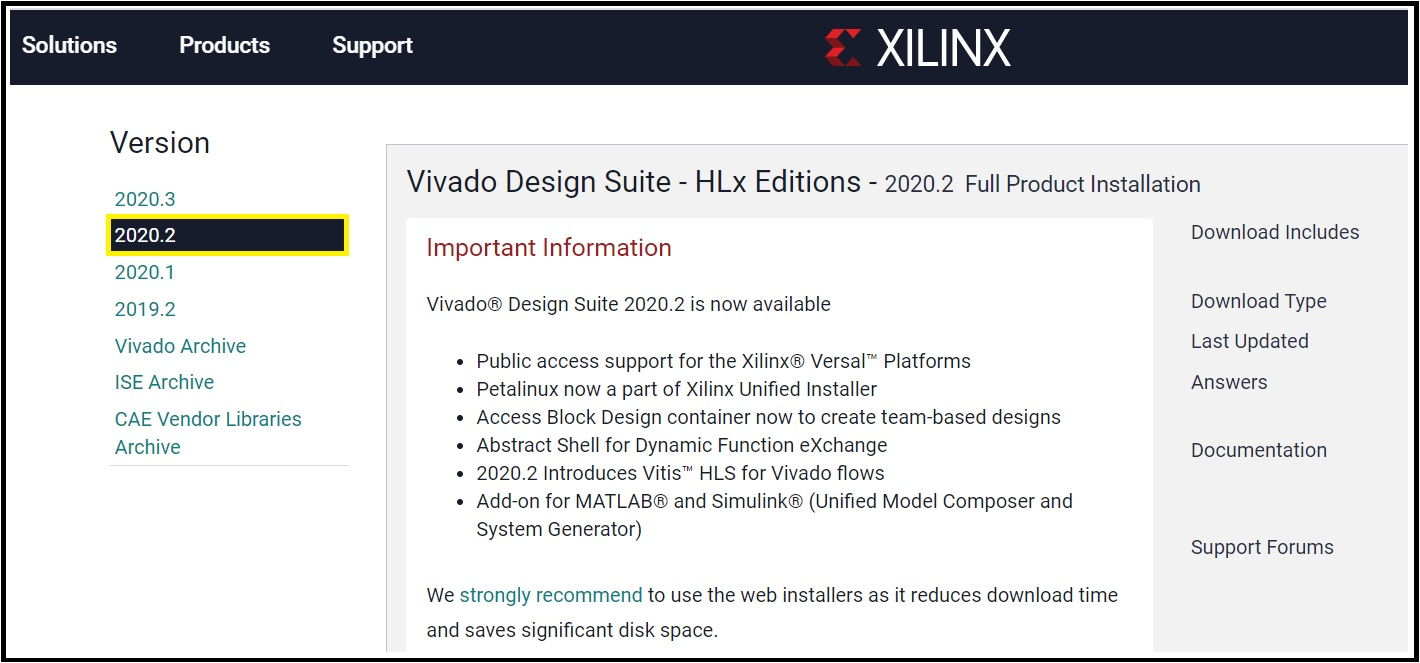
\includegraphics[width=\linewidth]{images/VivadoInstimg002.jpg}
  \end{center}
  Opmerking: sommige gebruikers hebben nog succes met oudere versies, omdat het hoofddoel hier is om een versie te installeren die de FPGA van uw doelhardware ondersteunt. \\
  \\
  Dat wil zeggen de Artix7 100T (voor Nexys en R2) of 200T (R3/R3A/R4).
\end{minipage}

\begin{minipage}{\linewidth}
  Klik op Xilinx Unified Installer 2020.2: Windows Self Extracting Web Installer EXE - 248.44MB
  \\
  \begin{center}
    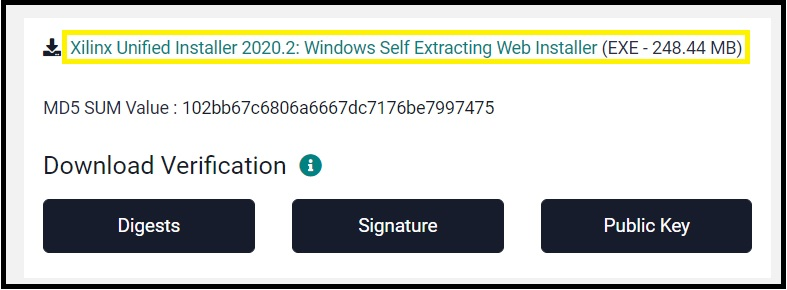
\includegraphics[width=0.8\linewidth]{images/VivadoInstimg003.jpg}
  \end{center}
\end{minipage}

\begin{minipage}{\linewidth}
  U wordt gevraagd een account aan te maken om in te kunnen loggen en het installatieprogramma te kunnen downloaden. \\
  \\
  Uw inloggegevens worden ook gevraagd tijdens de installatie.
  \\
  \begin{center}
    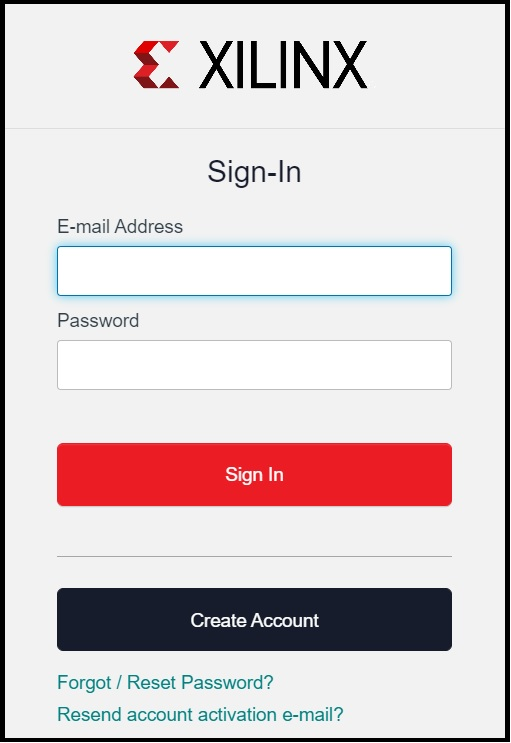
\includegraphics[width=0.3\linewidth]{images/VivadoInstimg004.jpg}
  \end{center}
\end{minipage}

\begin{minipage}{\linewidth}
  Nadat u ingelogd bent, moet u enkele persoonlijke gegevens invullen en dan op Download klikken.
  \\
  \begin{center}
    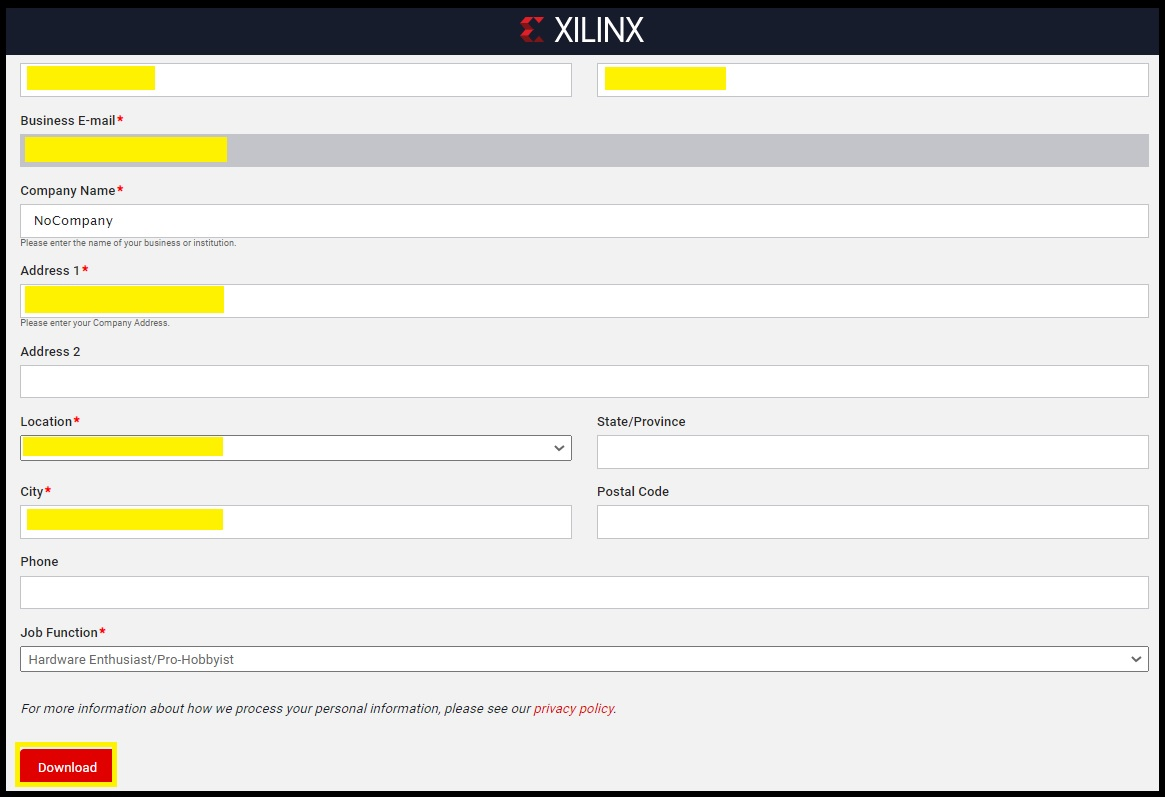
\includegraphics[width=0.8\linewidth]{images/VivadoInstimg005.jpg}
  \end{center}
\end{minipage}

\begin{minipage}{\linewidth}
  Voer het installatieprogramma uit als beheerder (Xilinx\_Unified\_2020.2\_1118\_1232\_Win64.exe).
  \\
  \begin{center}
    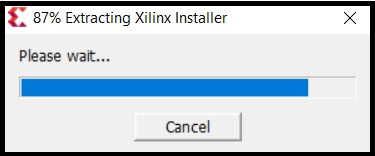
\includegraphics[width=0.5\linewidth]{images/VivadoInstimg006.jpg}
  \end{center}
\end{minipage}

\begin{minipage}{\linewidth}
  Klik op Allow Access.
  \\
  \begin{center}
    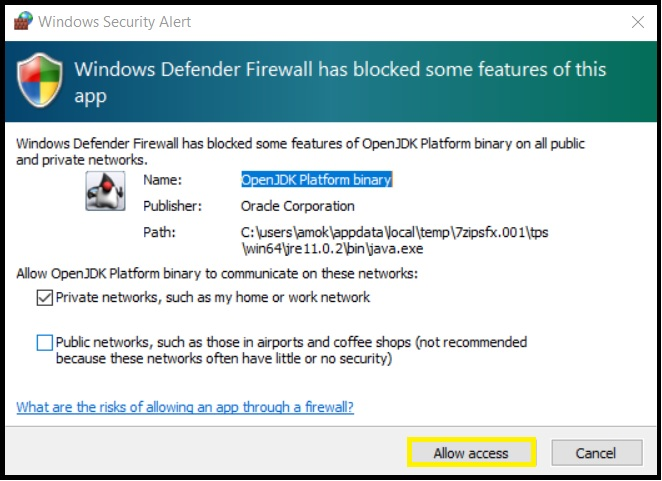
\includegraphics[width=0.5\linewidth]{images/VivadoInstimg007.jpg}
  \end{center}
\end{minipage}

\begin{minipage}{\linewidth}
  Klik op Next.
  \\
  \begin{center}
    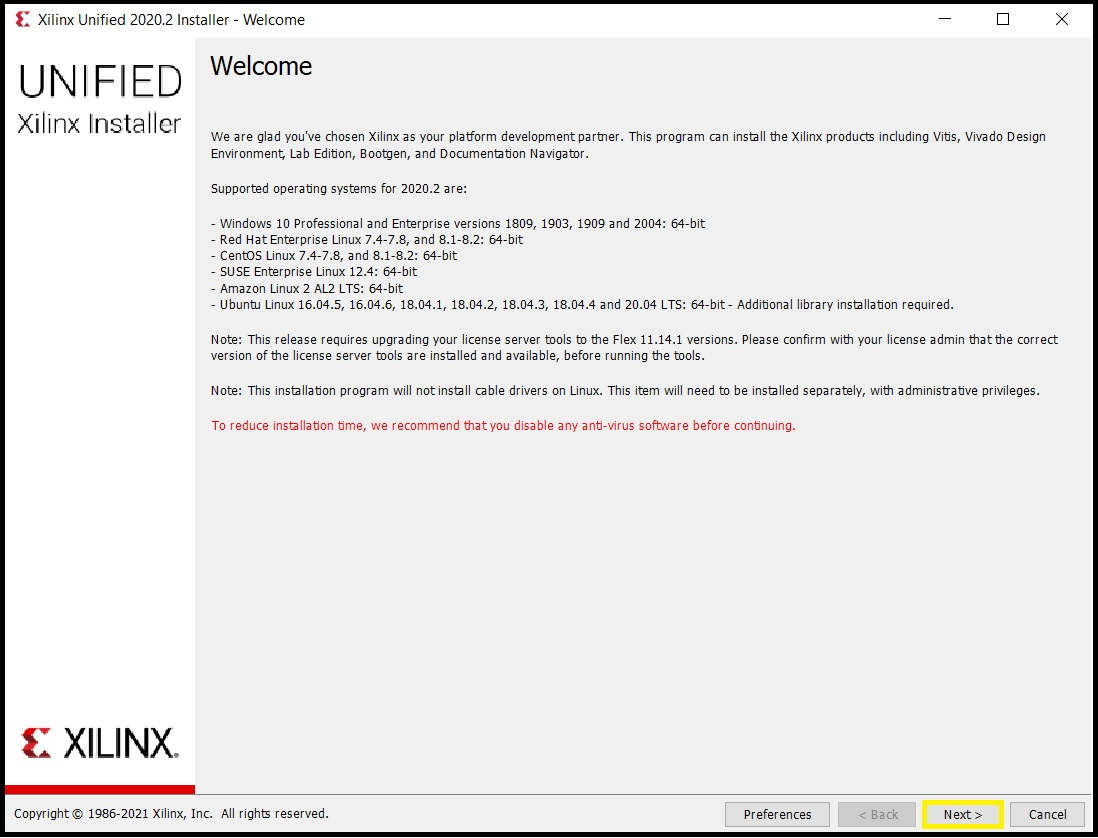
\includegraphics[width=0.7\linewidth]{images/VivadoInstimg008.jpg}
  \end{center}
\end{minipage}

\begin{minipage}{\linewidth}
  Voer uw inloggegevens in en klik op Next.
  \\
  \begin{center}
    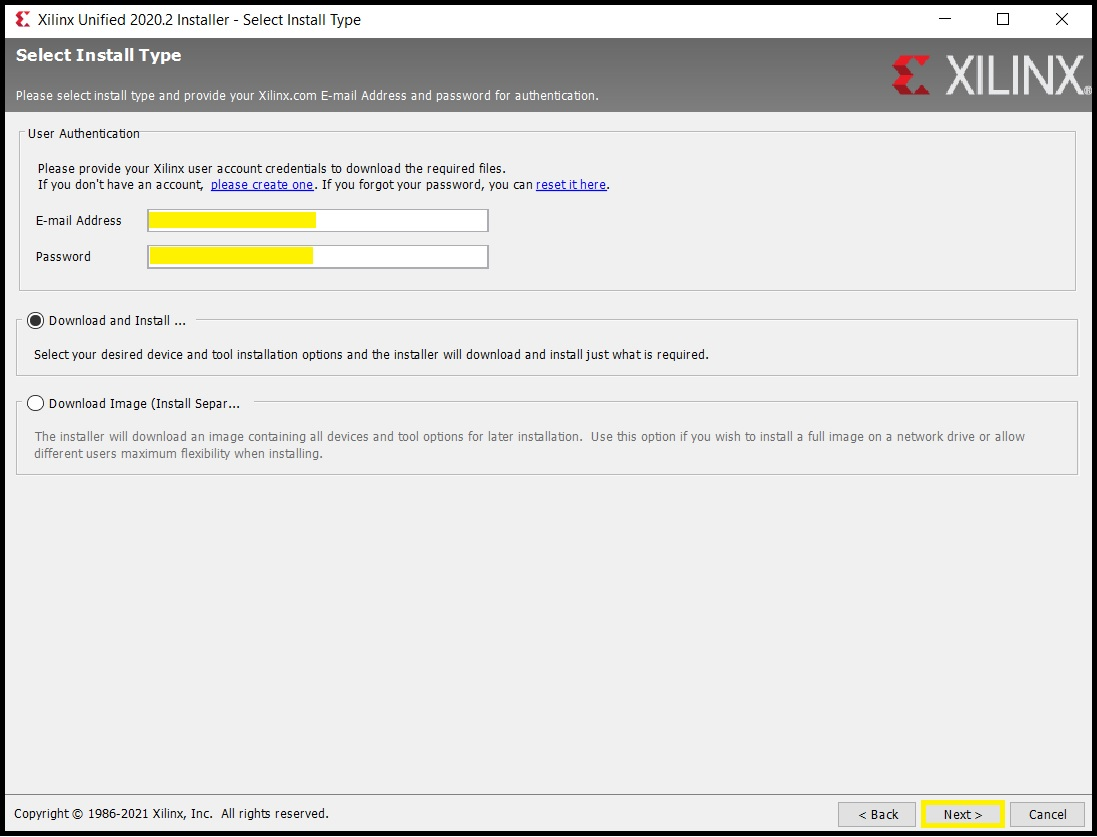
\includegraphics[width=0.7\linewidth]{images/VivadoInstimg009.jpg}
  \end{center}
\end{minipage}

\begin{minipage}{\linewidth}
  Selecteer Vivado en klik op Next.
  \\
  \begin{center}
    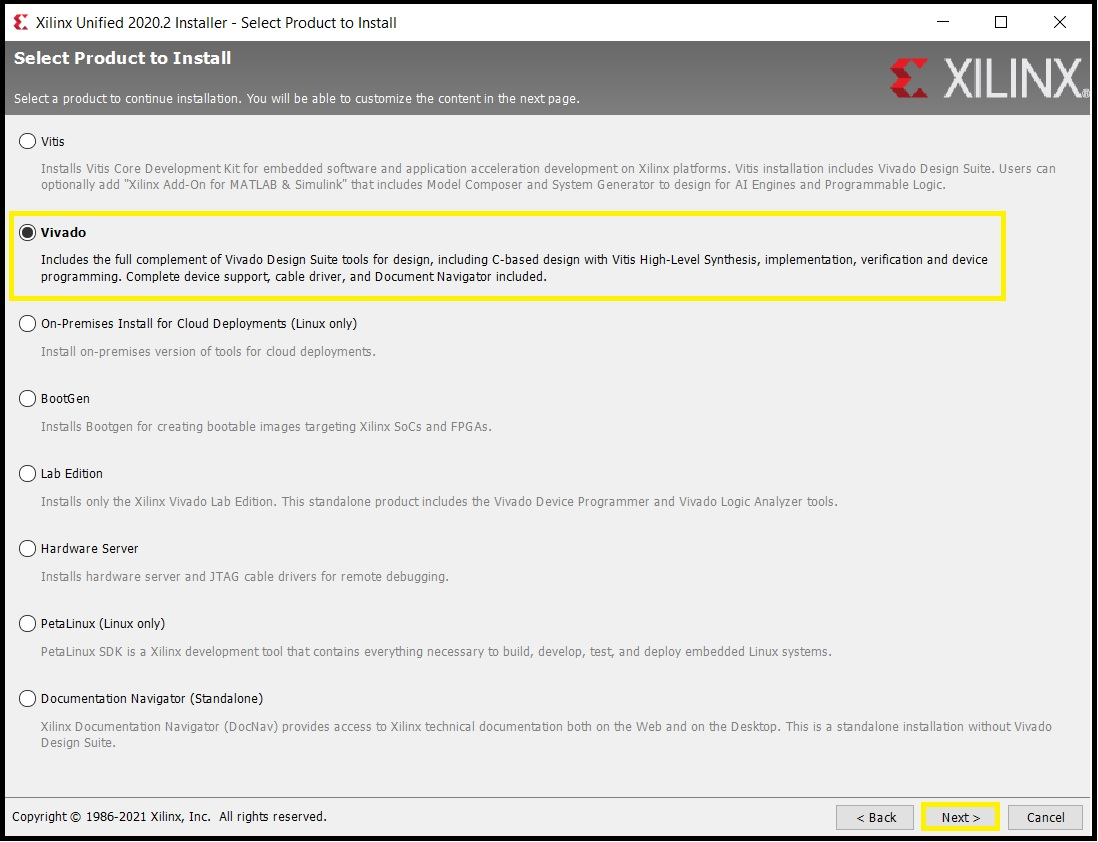
\includegraphics[width=0.7\linewidth]{images/VivadoInstimg010.jpg}
  \end{center}
\end{minipage}

\begin{minipage}{\linewidth}
  Selecteer ``Vivado HL WebPACK'' en klik op ``Next''.
  \\
  \begin{center}
    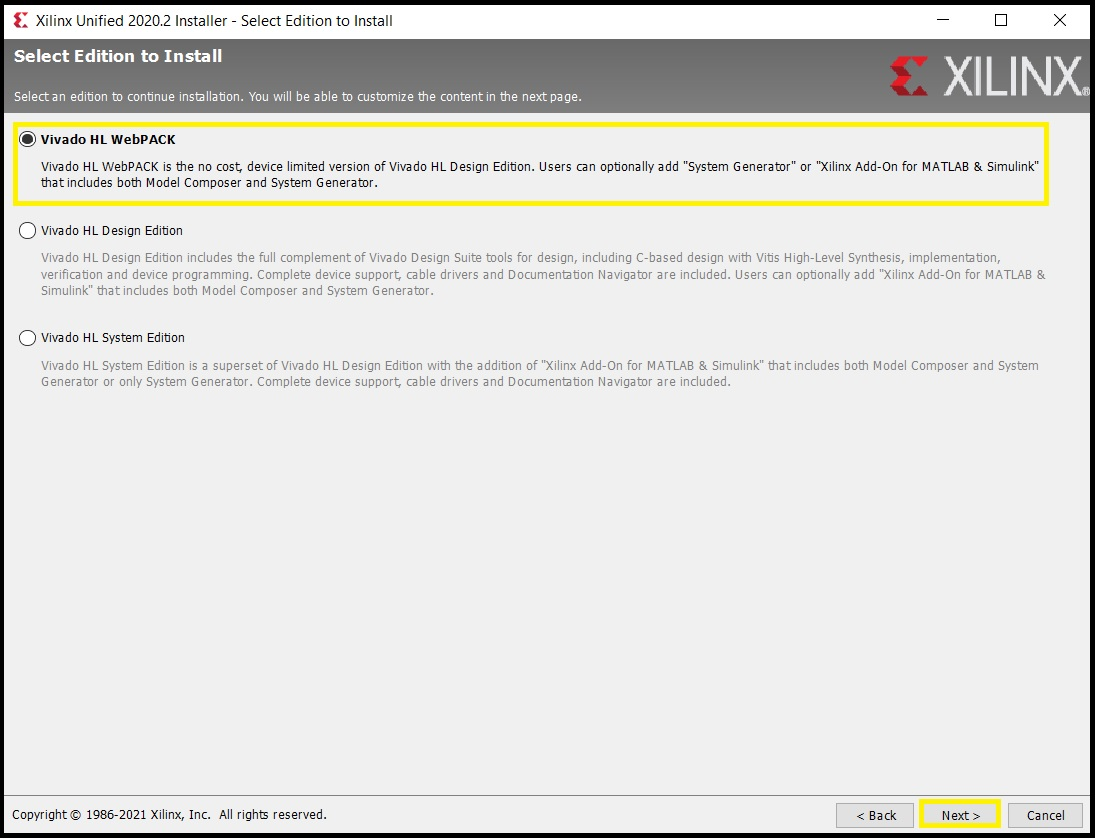
\includegraphics[width=0.7\linewidth]{images/VivadoInstimg011.jpg}
  \end{center}
\end{minipage}

\begin{minipage}{\linewidth}
  Wij raden aan om alleen de apparaten uit de ``\textbf{7 Series}'' te selecteren, omdat onze gekozen FPGA in deze serie valt, en het deselecteren van de andere series bespaart u ongeveer 6 GB aan downloadgrootte. Klik dan op ``Next''.
  \\
  \begin{center}
    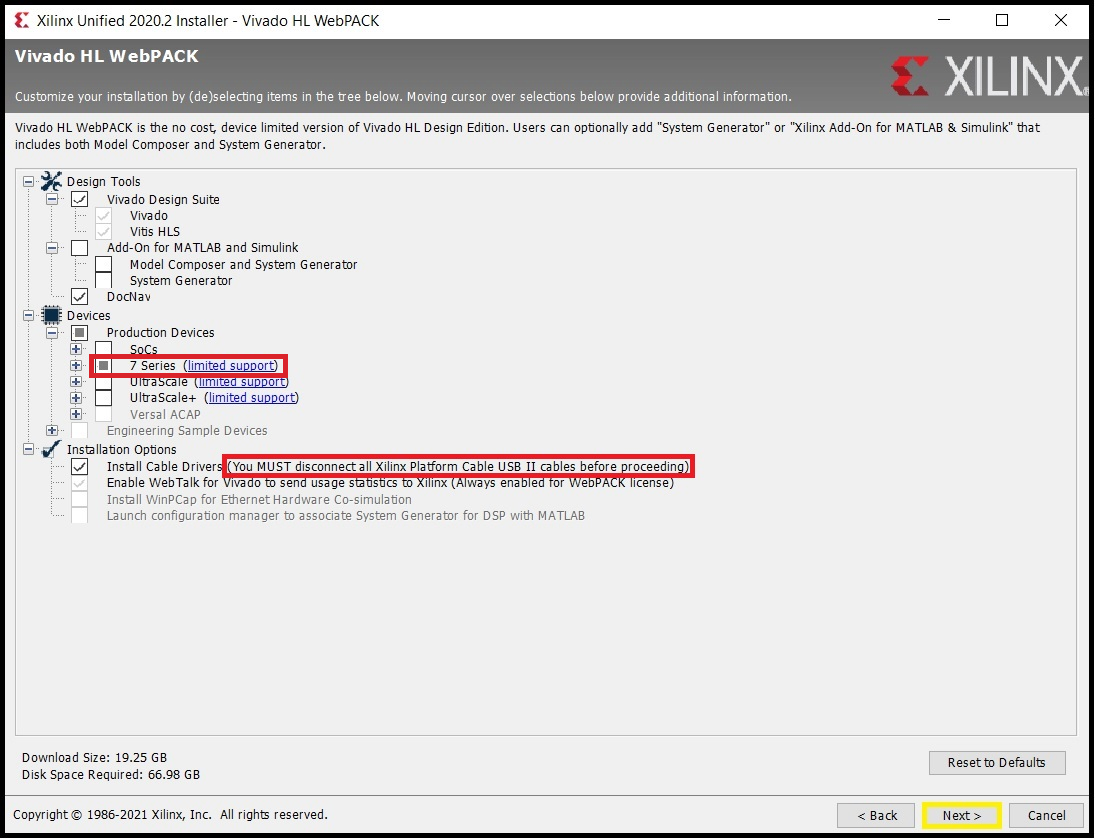
\includegraphics[width=0.7\linewidth]{images/VivadoInstimg012.png}
  \end{center}
  Waarschuwing: zoals gezegd, ontkoppel elke USB-kabel die op uw pc is aangesloten van het Nexys-bord.
\end{minipage}

\begin{minipage}{\linewidth}
  Ga akkoord met alle bepalingen van de eindgebruikerslicentieovereenkomst en de voorwaarden en klik op ``Next''.
  \\
  \begin{center}
    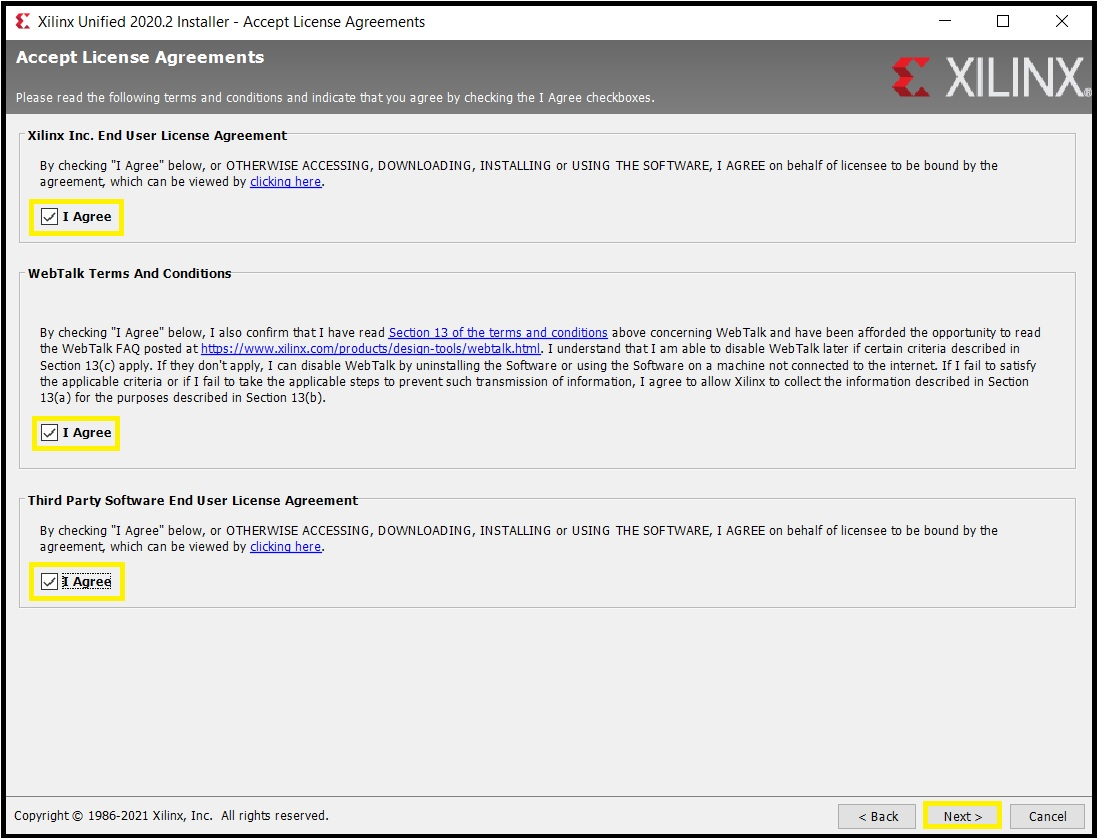
\includegraphics[width=0.7\linewidth]{images/VivadoInstimg013.jpg}
  \end{center}
\end{minipage}

\begin{minipage}{\linewidth}
  Kies de locatie waar u de software wilt installeren en klik op ``Next''.
  \\
  \begin{center}
    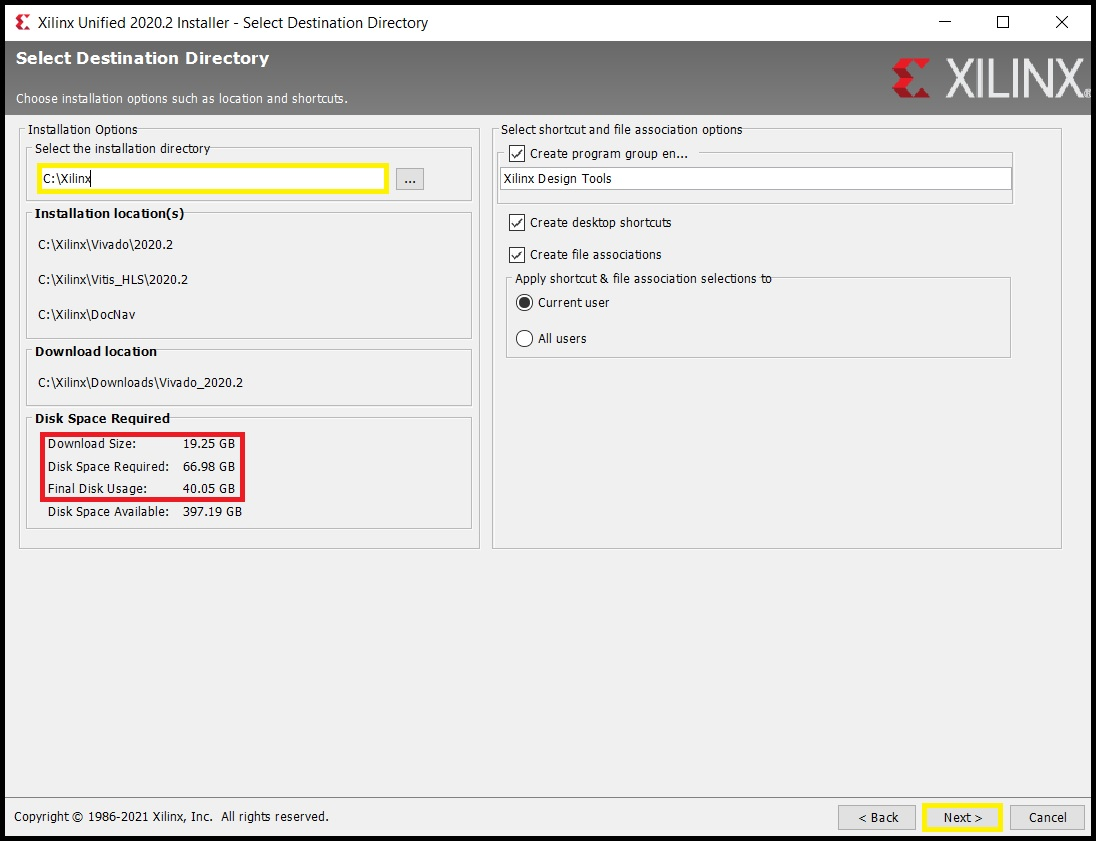
\includegraphics[width=0.7\linewidth]{images/VivadoInstimg014.jpg}
  \end{center}
  Waarschuwing: u staat op het punt om 20 GB aan software te downloaden en u hebt 70 GB nodig om de installatie uit te voeren.
\end{minipage}

\begin{minipage}{\linewidth}
  Klik op ``Yes''.
  \\
  \begin{center}
    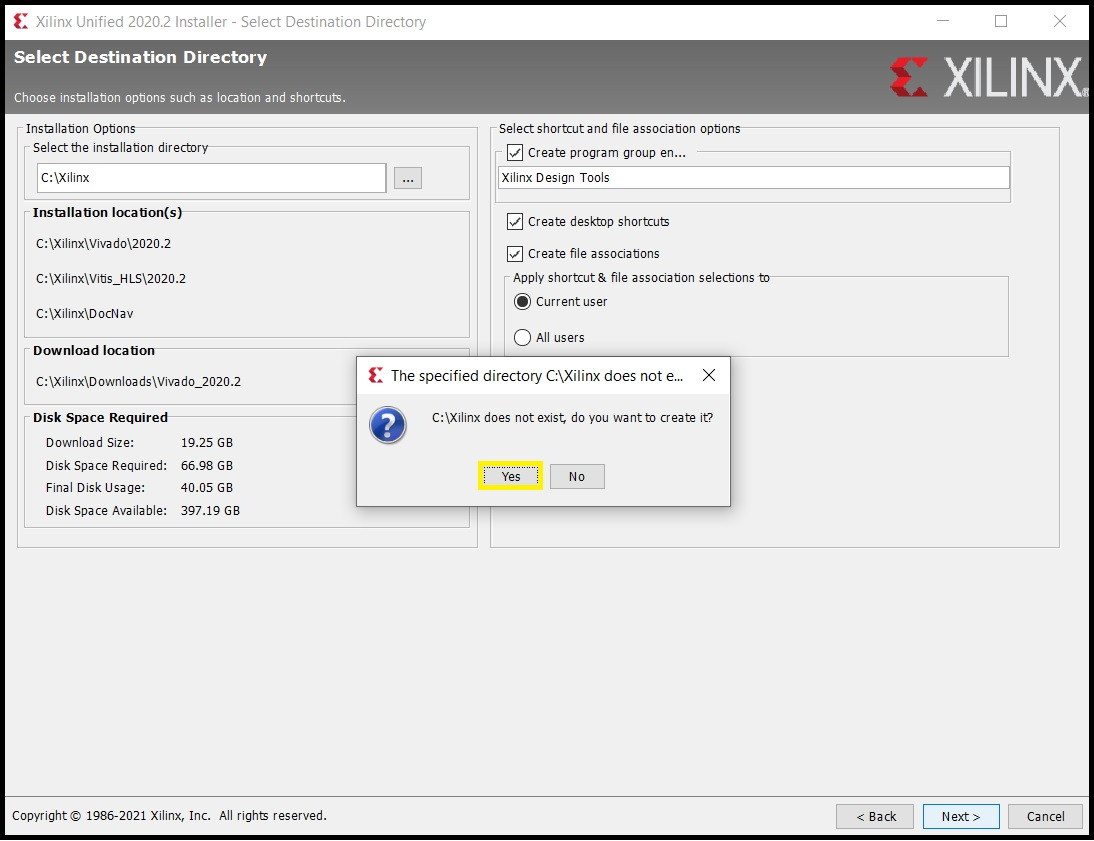
\includegraphics[width=0.7\linewidth]{images/VivadoInstimg015.jpg}
  \end{center}
\end{minipage}

\begin{minipage}{\linewidth}
  Klik op ``Install''.
  \\
  \begin{center}
    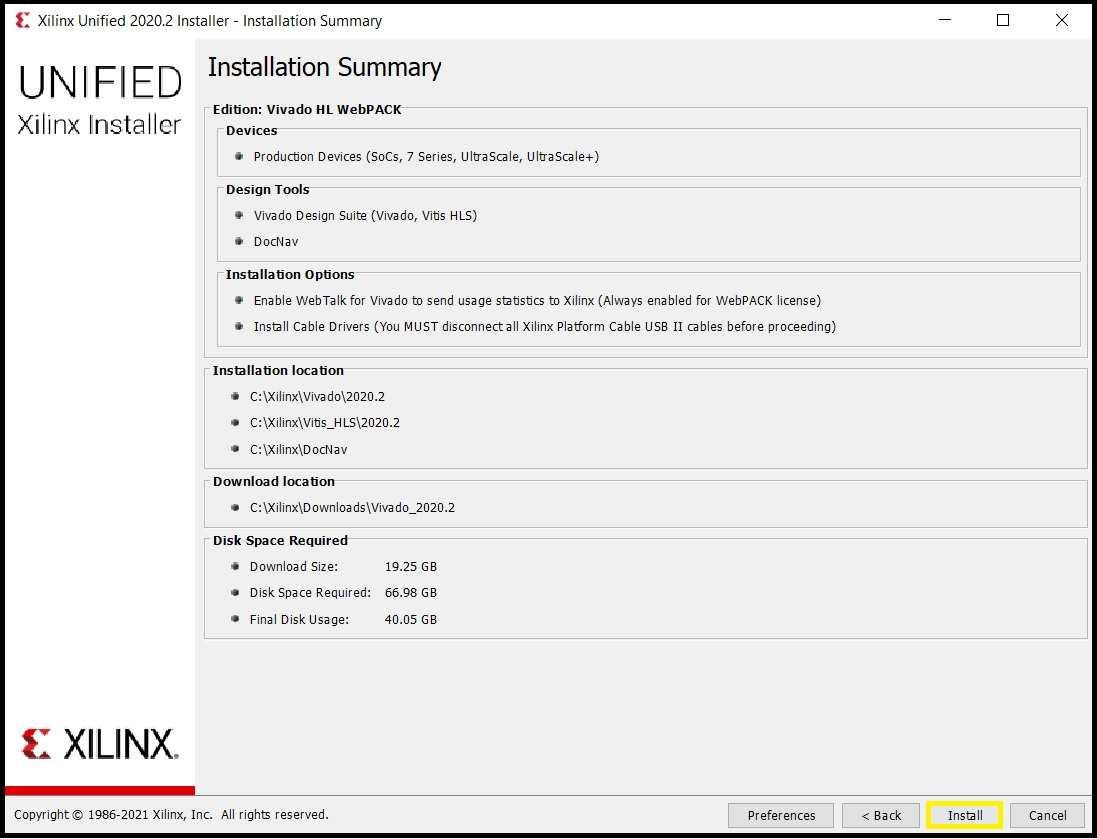
\includegraphics[width=0.7\linewidth]{images/VivadoInstimg016.jpg}
  \end{center}
\end{minipage}

\begin{minipage}{\linewidth}
  Wacht tot de installatie is voltooid. Aan het einde van de installatie wordt u gevraagd of u de Xilinx-apparatensoftware wilt installeren.
  \\
  \begin{center}
    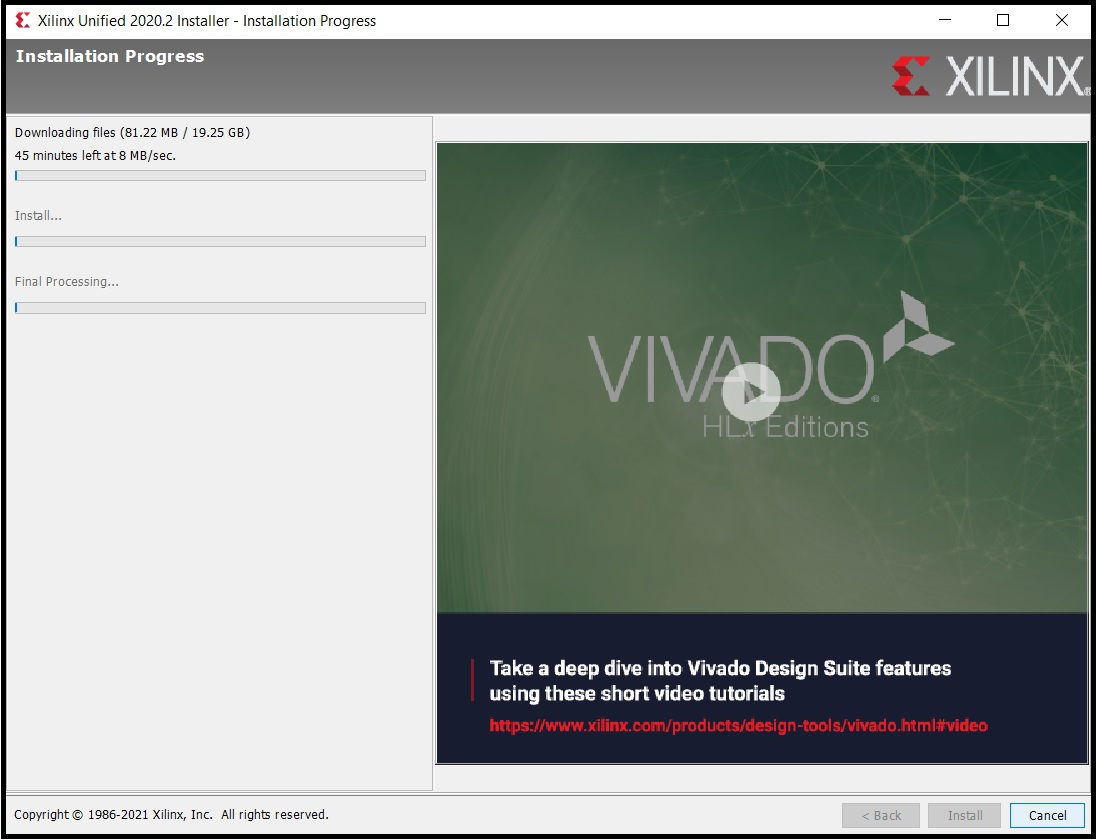
\includegraphics[width=0.7\linewidth]{images/VivadoInstimg017.jpg}
  \end{center}
\end{minipage}

\begin{minipage}{\linewidth}
  Klik op ``Install''.
  \\
  \begin{center}
    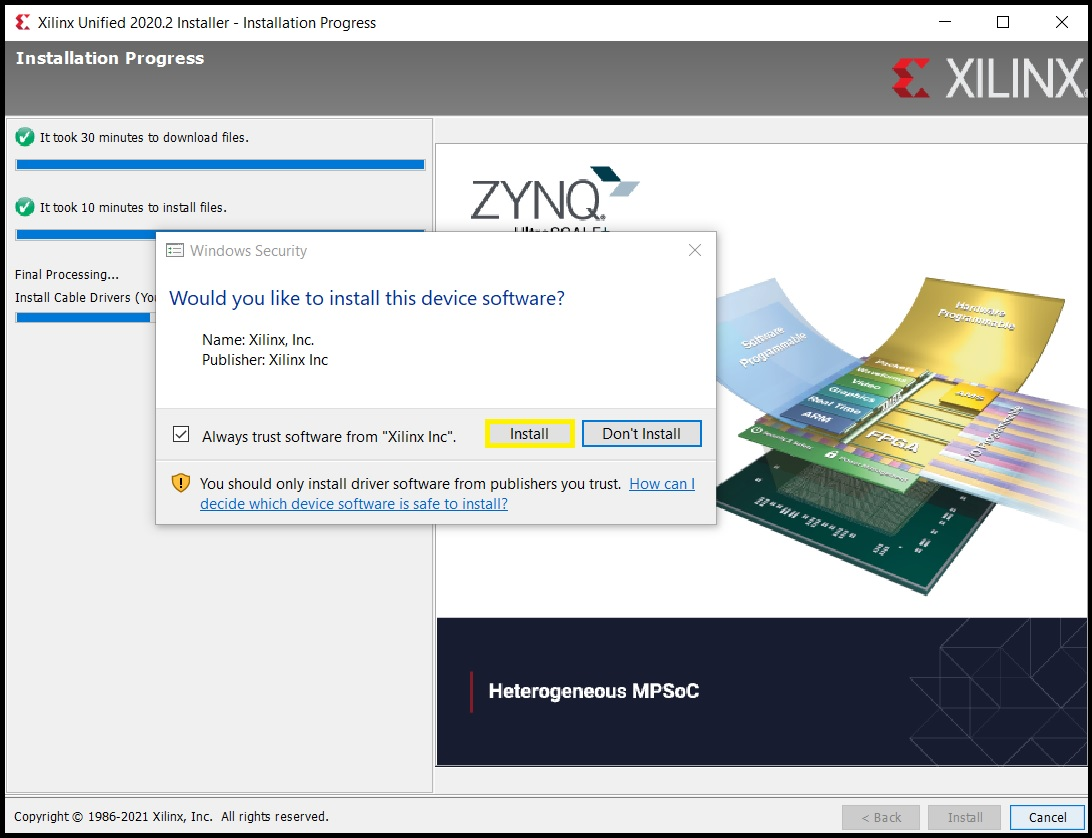
\includegraphics[width=0.7\linewidth]{images/VivadoInstimg018.jpg}
  \end{center}
  Laat de installatie voltooien.
\end{minipage}

\begin{minipage}{\linewidth}
  De installatie is voltooid. Klik op ``OK''.
  \\
  \begin{center}
    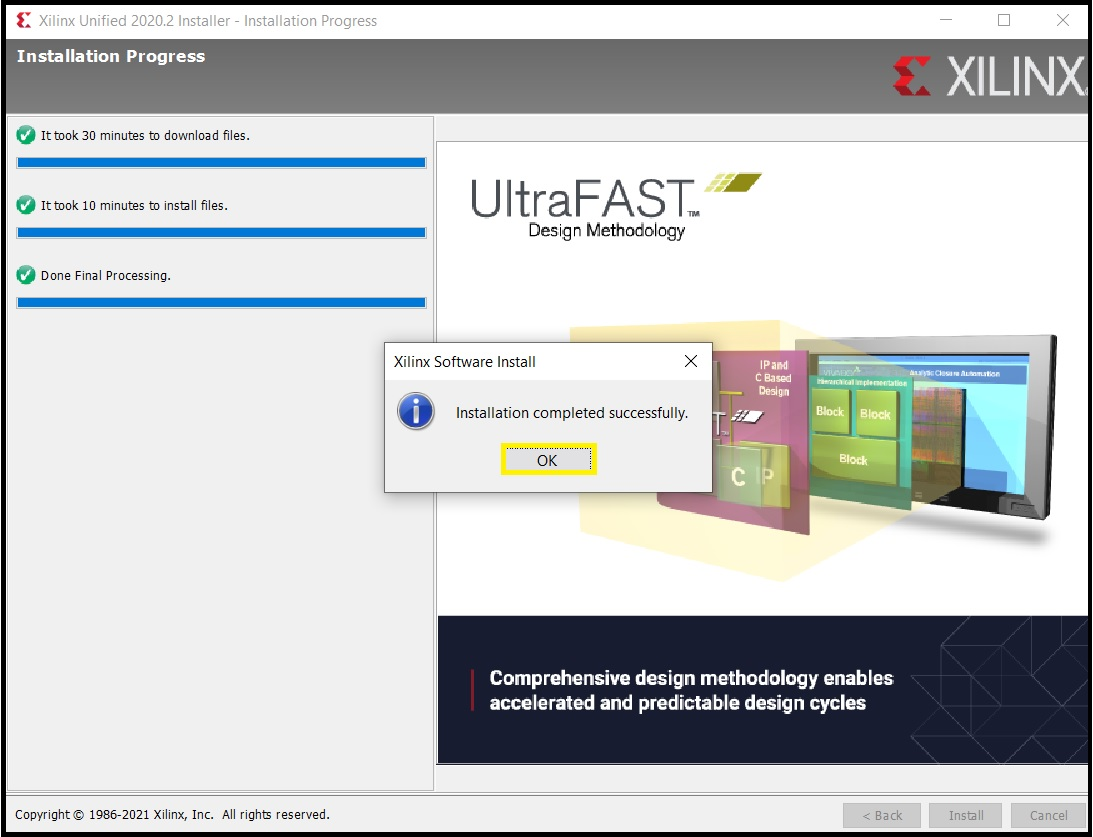
\includegraphics[width=0.7\linewidth]{images/VivadoInstimg019.jpg}
  \end{center}
\end{minipage}

\begin{minipage}{\linewidth}
  Op uw bureaublad verschijnen nu de volgende pictogrammen:
  \\
  \begin{center}
    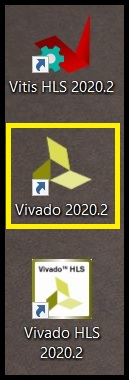
\includegraphics[width=0.2\linewidth]{images/VivadoInstimg020.jpg}
  \end{center}
  Let op: Ubuntu-gebruikers moeten mogelijk een ontbrekende afhankelijkheid installeren met: {\tt sudo apt install libtinfo5}
\end{minipage}

\begin{minipage}{\linewidth}
  Start Vivado 2020.2
  \\
  \begin{center}
    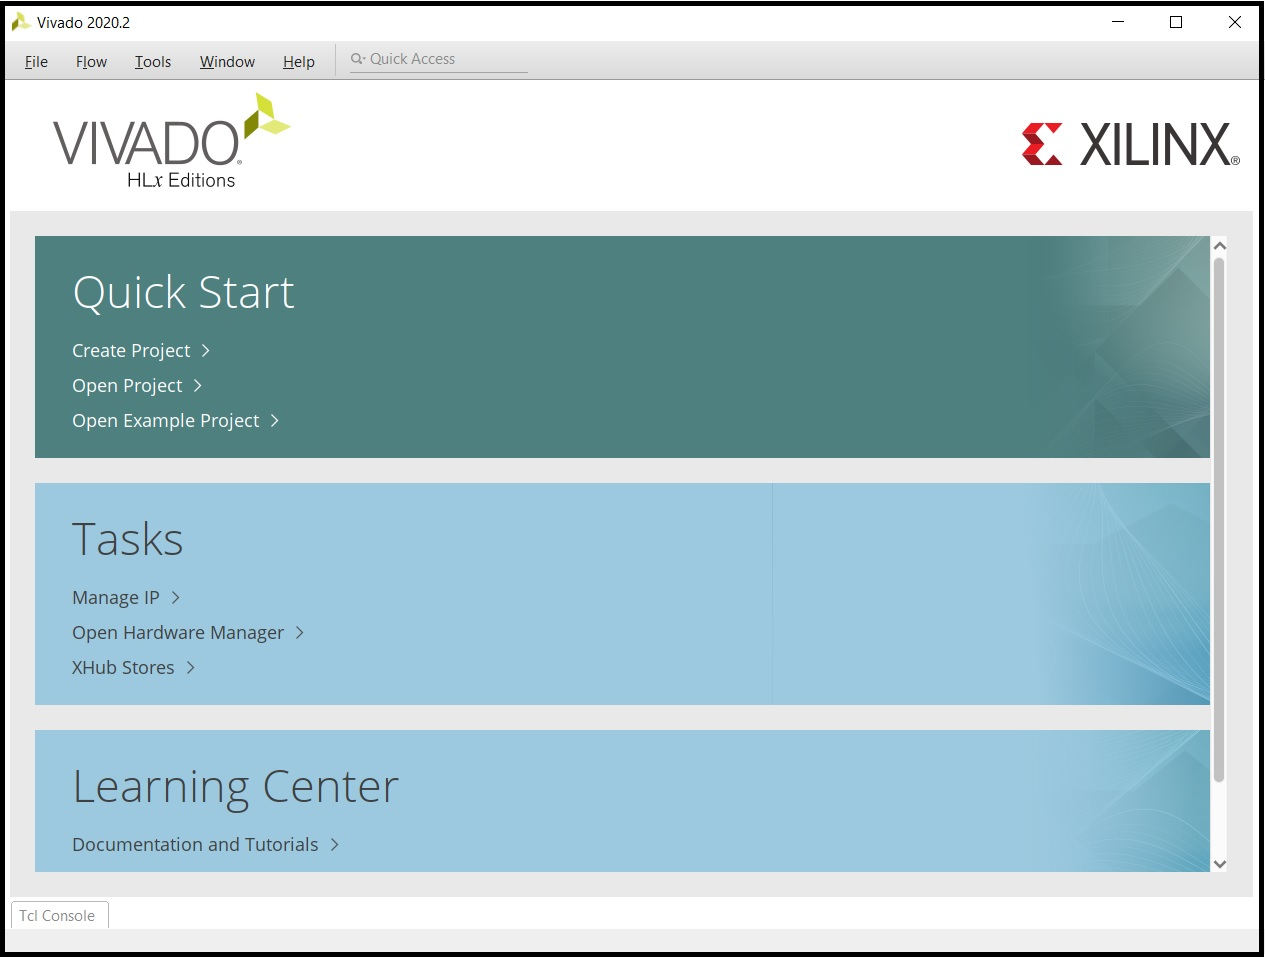
\includegraphics[width=0.7\linewidth]{images/VivadoInstimg021.jpg}
  \end{center}
\end{minipage}

\begin{minipage}{\linewidth}
  Klik op ``Help''->``Obtain a licence Key''.
  \\
  \begin{center}
    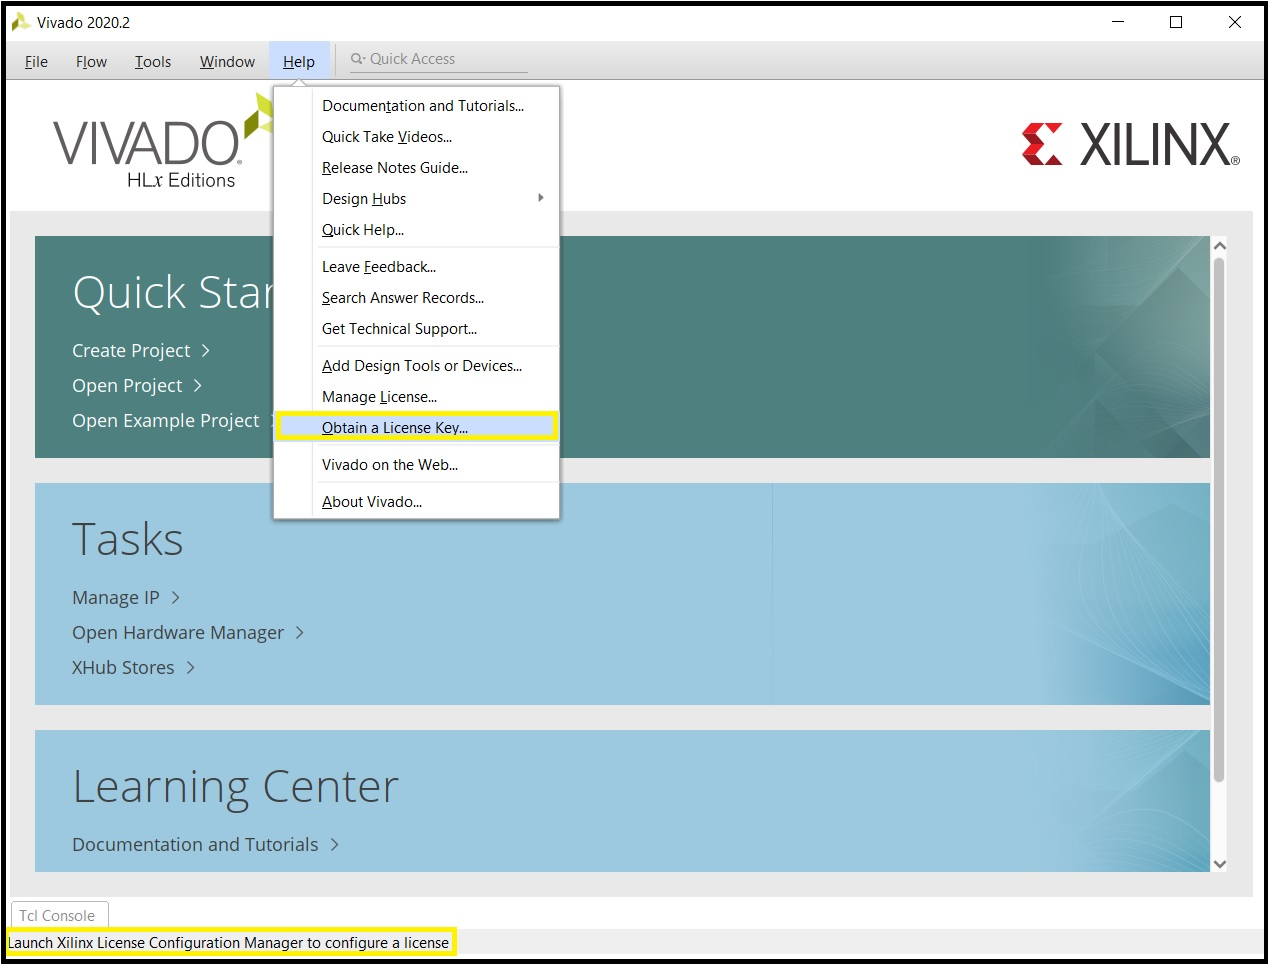
\includegraphics[width=0.7\linewidth]{images/VivadoInstimg022.jpg}
  \end{center}
\end{minipage}

\begin{minipage}{\linewidth}
  Hiermee opent u de Vivado-licentiemanager. \\
  \\
  Selecteer ``Get Free ISE WebPACK, ISE/Vivado IP or PetaLinux Licenses'' \\
  \\
  Klik op ``Connect Now''.
  \\
  \begin{center}
    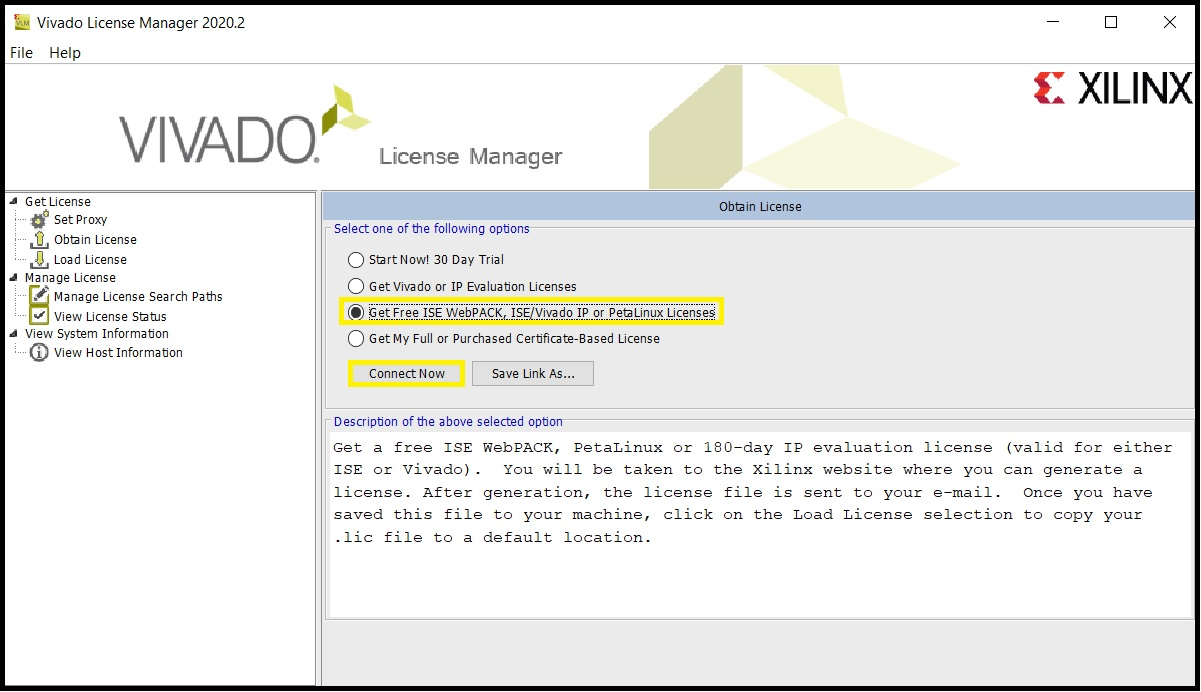
\includegraphics[width=\linewidth]{images/VivadoInstimg023.jpg}
  \end{center}
\end{minipage}

\begin{minipage}{\linewidth}
  Verbind met het gebruikersaccount dat u hebt aangemaakt om de Vivado-software te kunnen downloaden. Als u nog niet op de website van Xilinx was ingelogd, wordt u naar de hoofdpagina geleid. Keer terug naar de licentiemanager (die niet is gesloten).
  \\
  \begin{center}
    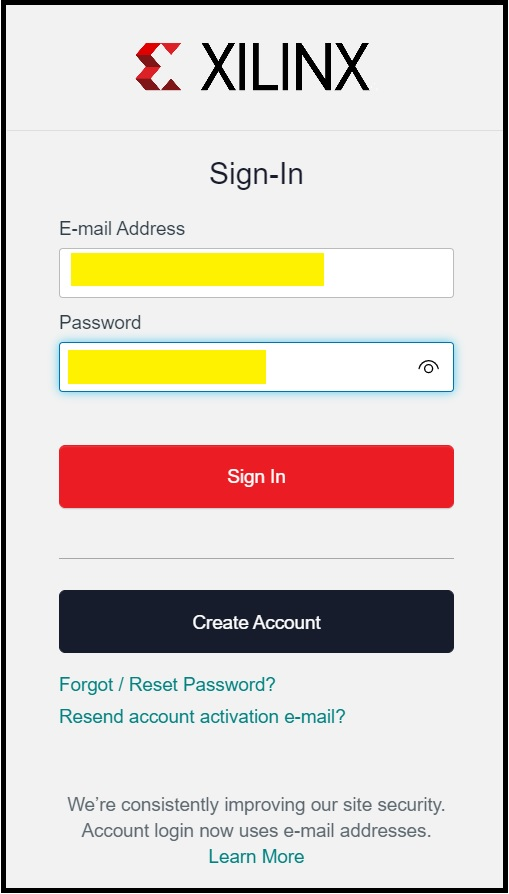
\includegraphics[width=0.3\linewidth]{images/VivadoInstimg024.jpg}
  \end{center}
\end{minipage}

\begin{minipage}{\linewidth}
  Klik opnieuw op ``Connect Now'' (controleer of ``Get Free ISE WebPACK, ISE/Vivado IP or PetaLinux Licenses'' nog steeds is geselecteerd).
  \\
  \begin{center}
    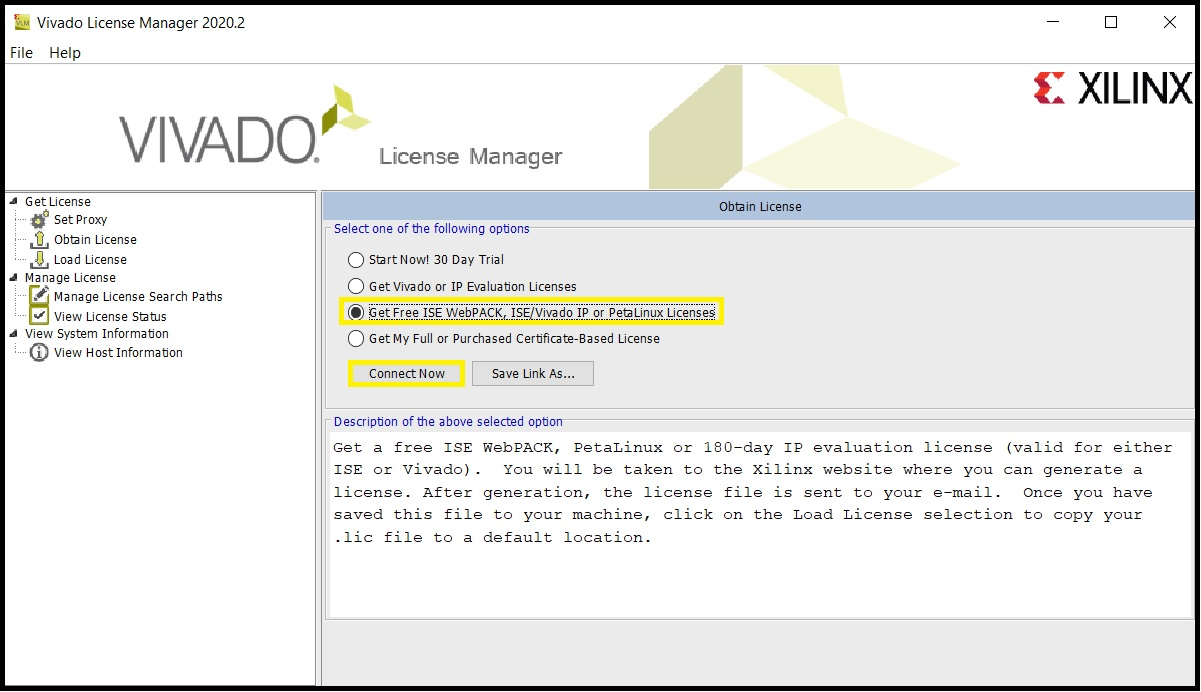
\includegraphics[width=\linewidth]{images/VivadoInstimg023.jpg}
  \end{center}
\end{minipage}

\begin{minipage}{\linewidth}
  Vervolgens registreert u uw persoonlijke gegevens op de Vivado-website en klikt u op ``Next''.
  \\
  \begin{center}
    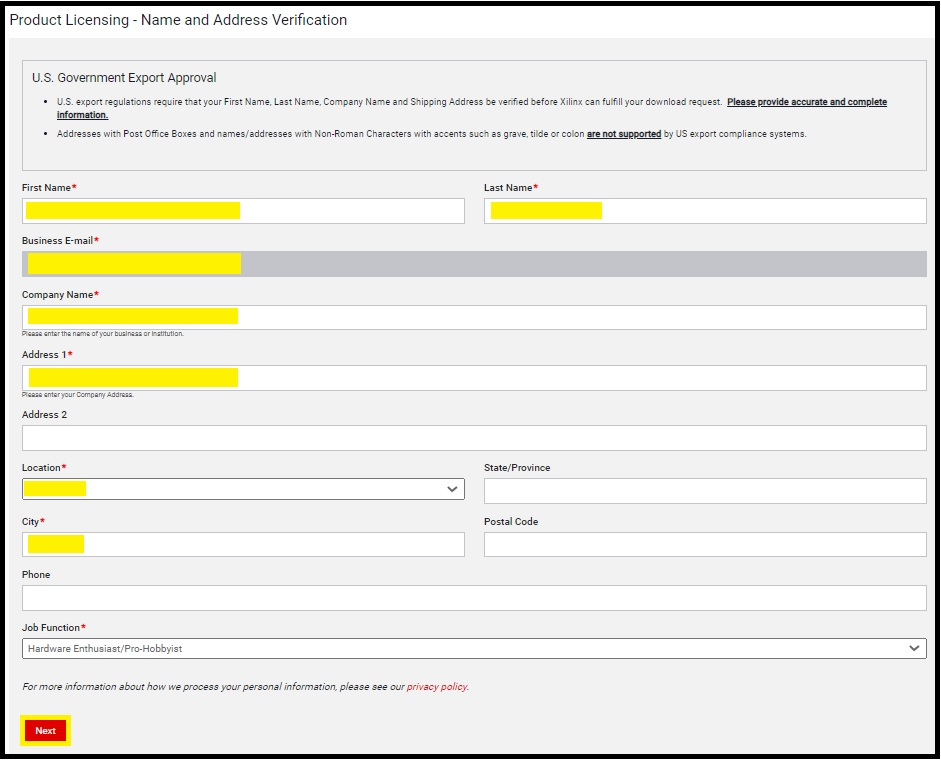
\includegraphics[width=0.7\linewidth]{images/VivadoInstimg025.jpg}
  \end{center}
\end{minipage}


\begin{minipage}{\linewidth}
Selecteer ``ISE WebPACK Licence'' en ``Vivado Design Suite: HL WebPACK 2015 and Earlier License'' \\
\\
Klik vervolgens op ``Generate Node-Locked Licence''.
\\
\begin{center}
  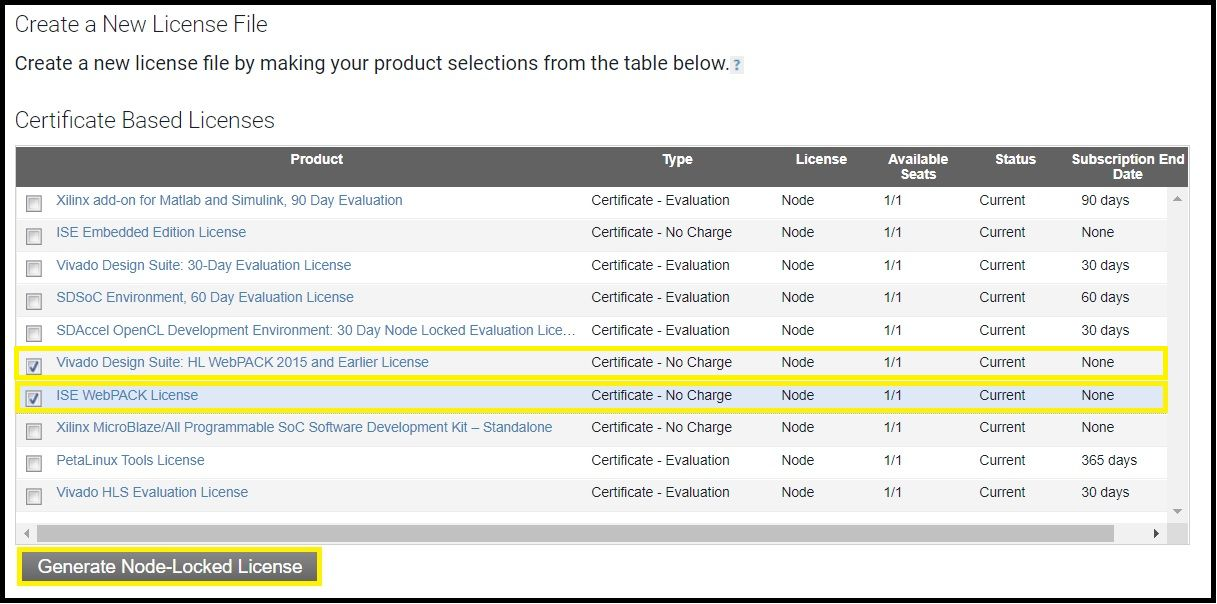
\includegraphics[width=\linewidth]{images/VivadoInstimg026.jpg}
\end{center}
\end{minipage}

\begin{minipage}{\linewidth}
  Klik op ``Next''.
  \\
  \begin{center}
    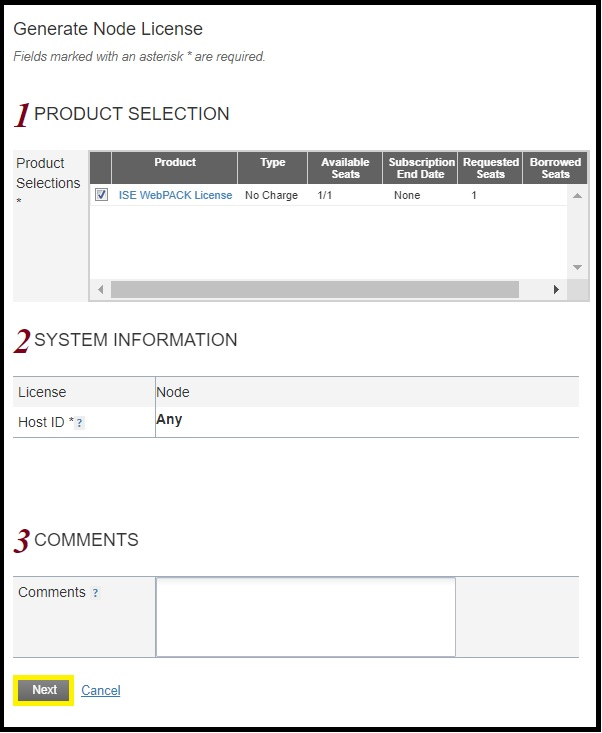
\includegraphics[width=0.5\linewidth]{images/VivadoInstimg027.jpg}
  \end{center}
\end{minipage}

\begin{minipage}{\linewidth}
  Klik op ``Next''.
  \\
  \begin{center}
    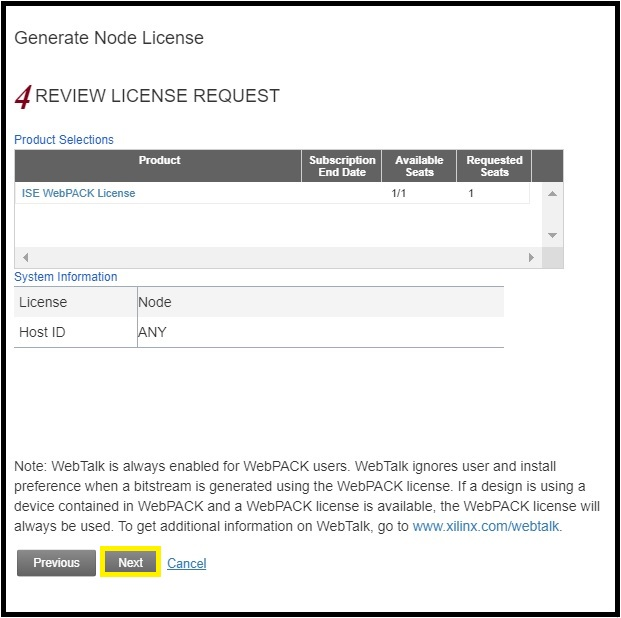
\includegraphics[width=0.5\linewidth]{images/VivadoInstimg028.jpg}
  \end{center}
\end{minipage}


\begin{minipage}{\linewidth}
  Controleer uw e-mail: u hebt een e-mail ontvangen van Xilinx, Inc. met een licentiebestand met de naam ``Xilinc.lic'' als bijlage. \\
  \\
  Sla dit bestand op uw computer op en bewaar het op een veilige plaats.
  \\
  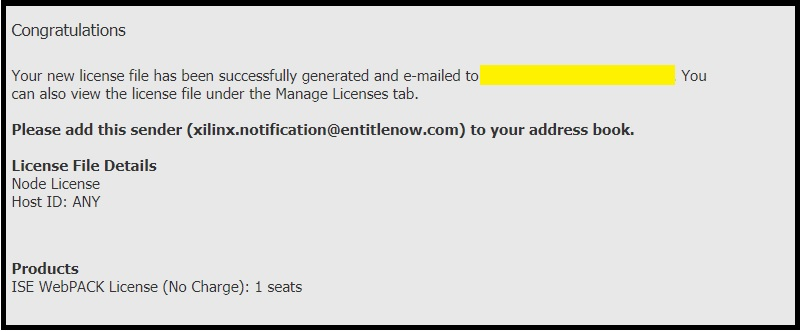
\includegraphics[width=\linewidth]{images/VivadoInstimg029.jpg}
\end{minipage}

\begin{minipage}{\linewidth}
  Ga terug naar de licentiemanager (die nog steeds actief is). \\
  \\
  Selecteer ``Load License'' en klik op ``Copy License''.
  \\
  \begin{center}
    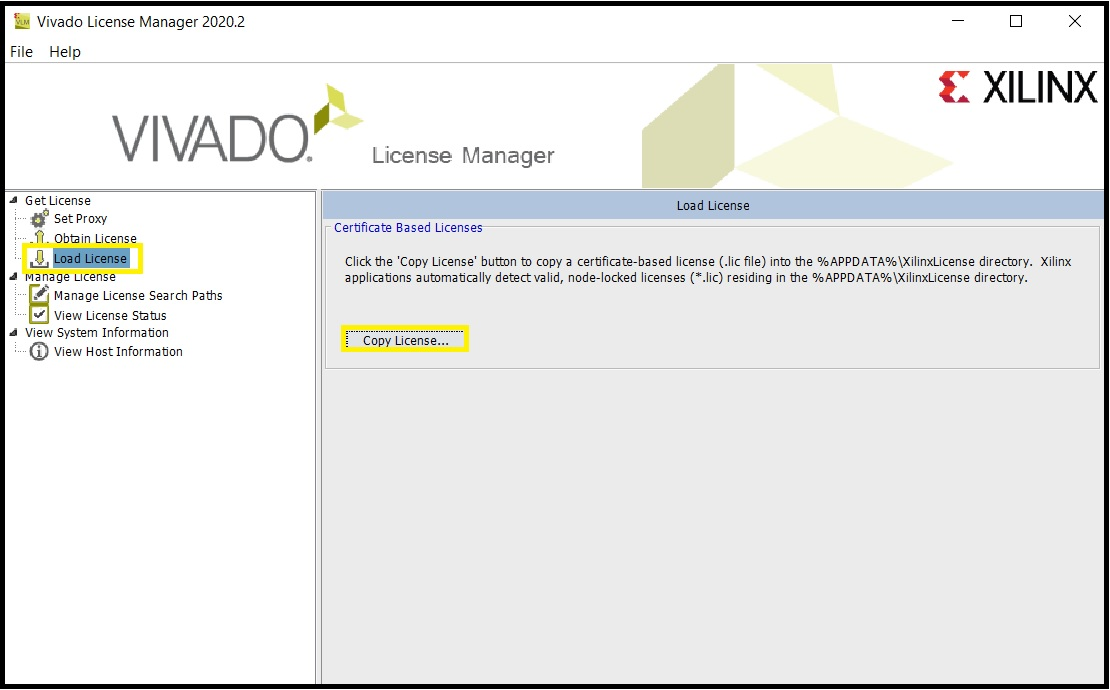
\includegraphics[width=0.8\linewidth]{images/VivadoInstimg030.jpg}
  \end{center}
\end{minipage}

\begin{minipage}{\linewidth}
  Blader naar de locatie waar u het bestand ``Xilinc.lic'' heeft opgeslagen, selecteer het en klik op ``Open''.
  \\
  \begin{center}
    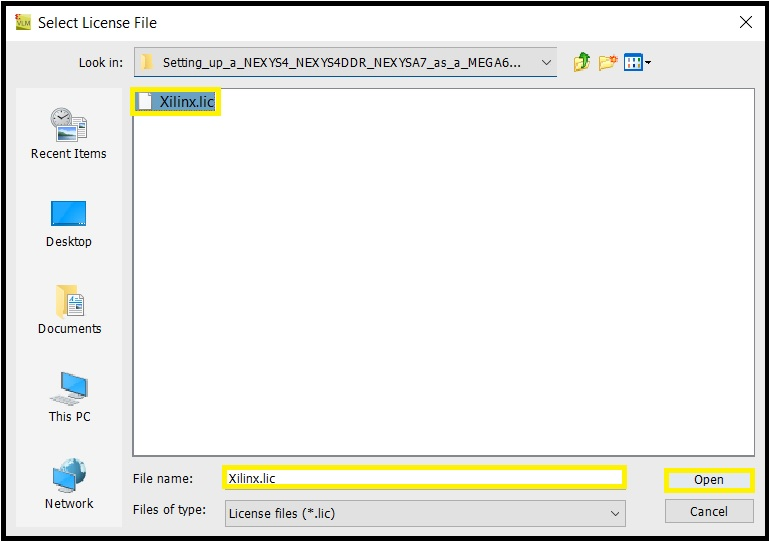
\includegraphics[width=0.7\linewidth]{images/VivadoInstimg031.jpg}
  \end{center}
\end{minipage}

\begin{minipage}{\linewidth}
  Klik op ``OK'' en sluit de Vivado-licentiemanager.
  \\
  \begin{center}
    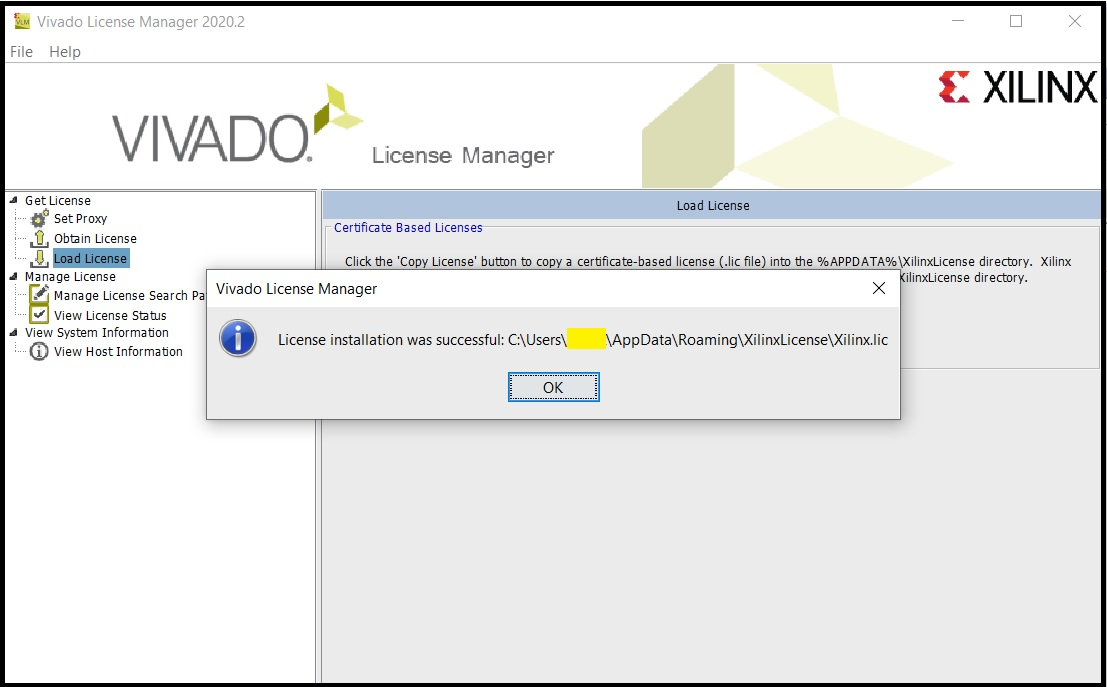
\includegraphics[width=0.7\linewidth]{images/VivadoInstimg032.jpg}
  \end{center}

  Uw Vivado-software is geregistreerd en u kunt deze nu gebruiken.
\end{minipage}

\section{De FTDI-stuurprogramma's installeren}

De FTDI-drivers zijn nodig om uw PC te laten communiceren met de JTAG-poort en de seriële communicatiepoort van de hardware (merk op dat de enkele fysieke USB-verbinding met uw PC feitelijk deze twee poorten aanbiedt).

\subsection{Linux-drivers}

Gebruikers van Linux melden dat zij de FTDI-drivers standaard in hun Linux-distributie aangetroffen hebben, terwijl anderen aangeven dat het volgende extra commando na de installatie van Vivado uitgevoerd moet worden:

cd /opt/Xilinx/Vivado/2018.3/data/xicom/cable\_drivers/lin64/install\_script/install\_drivers \\sudo ./install\_drivers

\subsection{Windows-drivers}

Download het volgende archief om de drivers te installeren:

\begin{itemize}
  \item \url{https://ftdichip.com/wp-content/uploads/2021/08/CDM212364_Setup.zip}
\end{itemize}

Pak het bestand \textbf{CDM212364\_Setup.zip} uit; u verkrijgt het bestand \textbf{CDM212364\_Setup.exe}.

\textcolor{red}{\underline{Waarschuwing}: \\Voordat u de drivers installeert, moet u de Nexys4-plaat uitschakelen en de USB-kabel loskoppelen van de PC.}

\begin{minipage}{\linewidth}
  Controleer welke apparaten er voor de installatie al aanwezig zijn:
  \\
  \begin{center}
    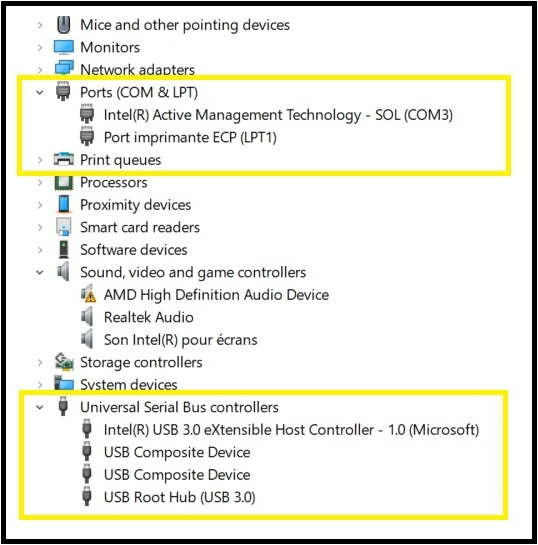
\includegraphics[width=0.6\linewidth]{images/img001_install_drivers_00.jpg}
  \end{center}
\end{minipage}

\begin{minipage}{\linewidth}
  Voer het bestand CDM212364\_Setup.exe uit als administrator:
  \\
  \begin{center}
    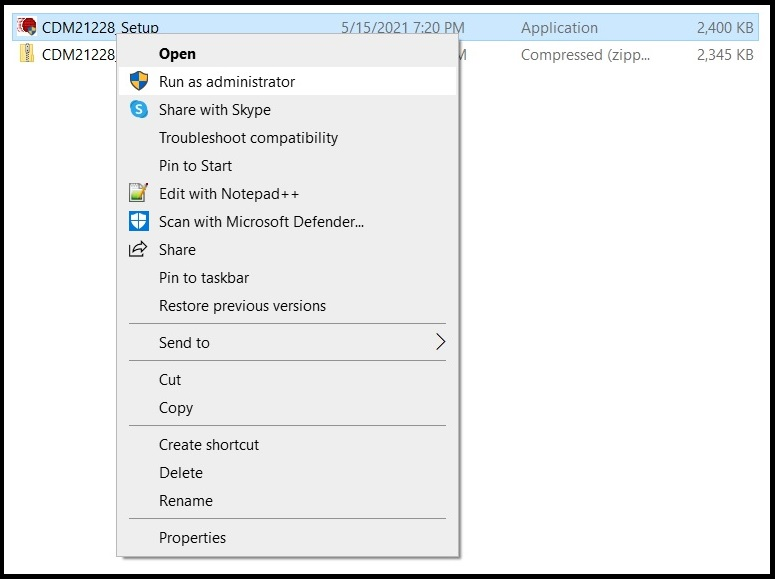
\includegraphics[width=0.6\linewidth]{images/img001_install_drivers_01.jpg}
  \end{center}
\end{minipage}

Bevestig dat u het programma wilt uitvoeren.

\begin{minipage}{\linewidth}
  Klik op ``Extract''.
  \\
  \begin{center}
    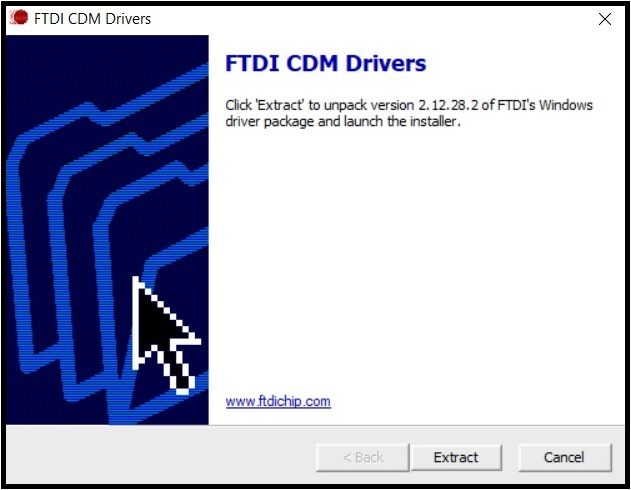
\includegraphics[width=0.6\linewidth]{images/img001_install_drivers_02.jpg}
  \end{center}
\end{minipage}

\begin{minipage}{\linewidth}
  Klik op ``Next >''.
  \\
  \begin{center}
    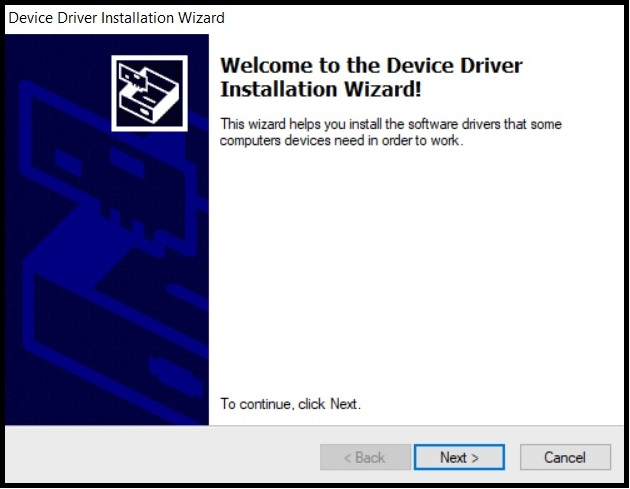
\includegraphics[width=0.6\linewidth]{images/img001_install_drivers_03.jpg}
  \end{center}
\end{minipage}

\begin{minipage}{\linewidth}
  Aanvaard de overeenkomst en klik op ``Next >''.
  \\
  \begin{center}
    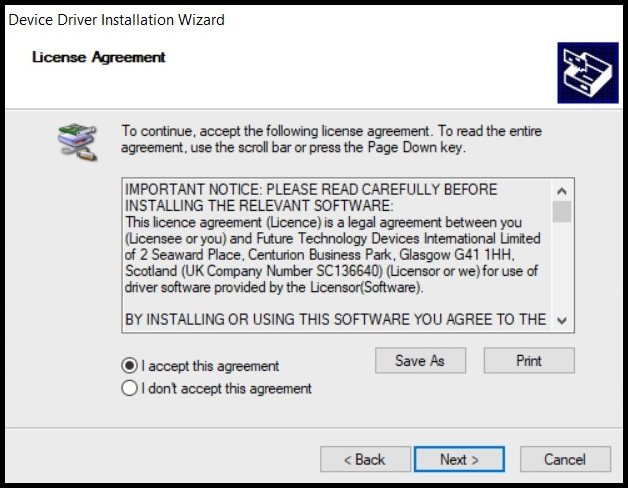
\includegraphics[width=0.6\linewidth]{images/img001_install_drivers_04.jpg}
  \end{center}
\end{minipage}

De installatie van de drivers wordt gestart.

\begin{minipage}{\linewidth}
  Klik op ``Finish''.
  \\
  \begin{center}
    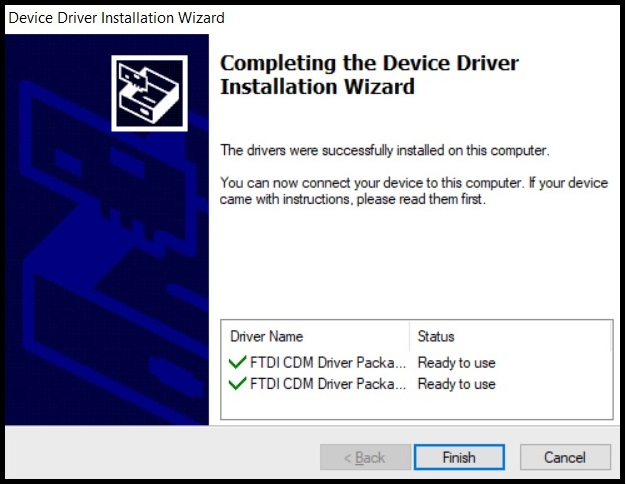
\includegraphics[width=0.6\linewidth]{images/img001_install_drivers_05.jpg}
  \end{center}
\end{minipage}

Sluit de USB-kabel aan op een USB-poort op de PC \textcolor{red}{zonder de Nexys4-plaat in te schakelen}.

Het aansluiten van de USB-kabel veroorzaakt het verschijnen van nieuwe apparaten.

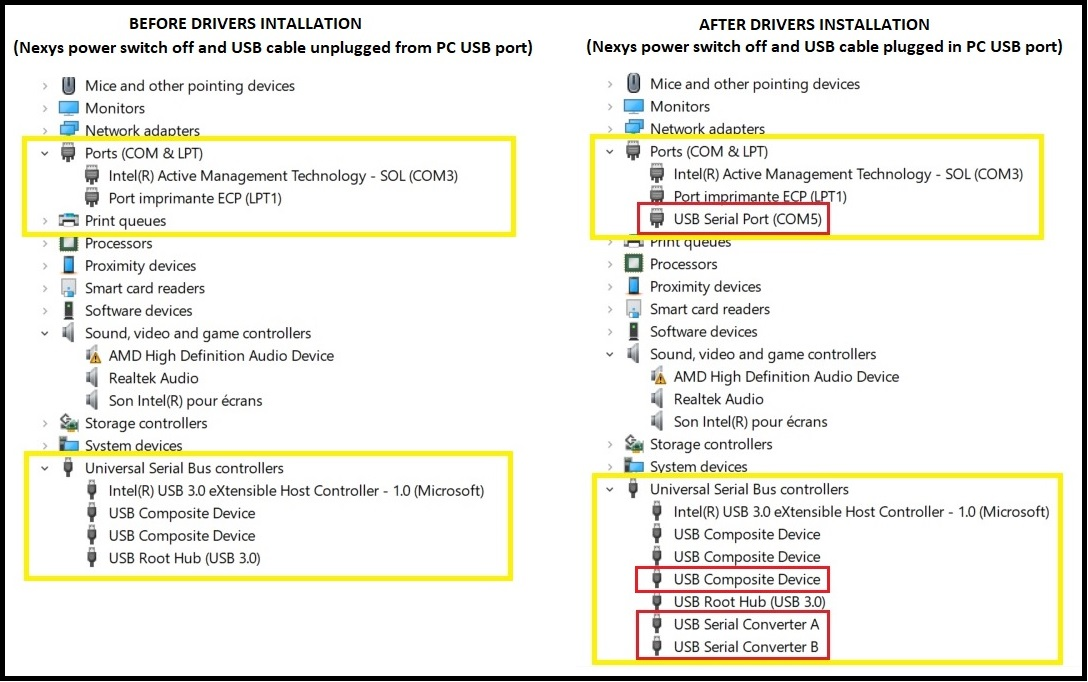
\includegraphics[width=\linewidth]{images/img001_install_drivers_07.jpg}

\begin{itemize}
  \item Er is een extra COM-poort geïnstalleerd: \textcolor{red}{dit is de COM-poort die gebruikt wordt om met de Nexys4-plaat te communiceren.}  \item Er is een extra USB-samengesteld apparaat geïnstalleerd.  \item Er zijn twee USB-serieel-omzetters geïnstalleerd.
\end{itemize}

Op dit moment is de Nexys4-plaat nog niet van stroom voorzien.

Voor meer informatie over de geïnstalleerde drivers kunt u de bijbehorende documentatie downloaden:

\begin{itemize}
  \item \url{https://ftdichip.com/wp-content/uploads/2020/08/AN\_396-FTDI-Drivers-Installation-Guide-for-Windows-10.pdf}
  \item \url{https://ftdichip.com/wp-content/uploads/2021/01/AN\_119\_FTDI\_Drivers\_Installation\_Guide\_for\_Windows7.pdf}
\end{itemize}

\section{De hoofd-FPGA flashen met Vivado}
\label{sec:mainfpgaflashing}

Ter verduidelijking: wanneer wij spreken over het ``flashen van de FPGA'', bedoelen wij in feite het flashen van het QSPI-flashgeheugen waarvan de FPGA bij het opstarten gebruikmaakt om de bitstream snel te laden.

De afbeelding hieronder toont twee veelgebruikte manieren waarop de FPGA bij het opstarten een bitstream kan laden:

\begin{center}
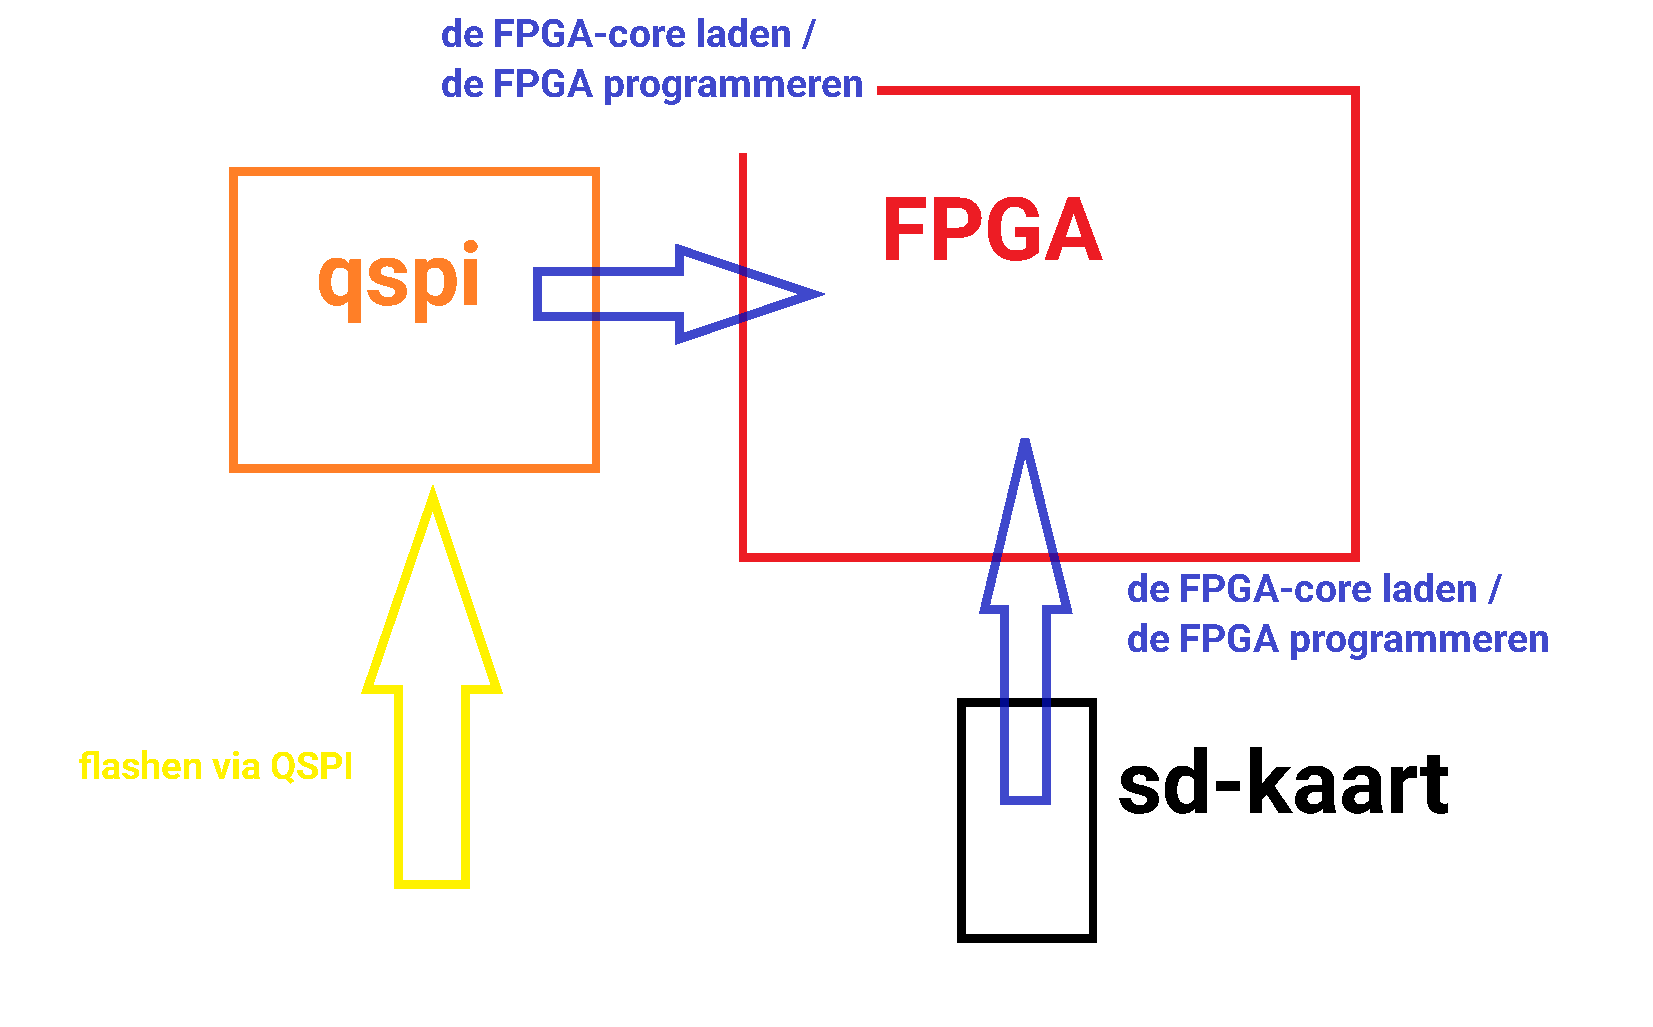
\includegraphics[width=0.8\linewidth]{dutch/images/flashing_fpga.pdf}
\end{center}

\begin{itemize}
  \item We kunnen eerst een bitstream-/core-bestand op het QSPI-flashgeheugen flashen, waarna de FPGA dit bij het opstarten snel kan laden. Het flashen van het QSPI is tamelijk traag, maar het voordeel van een korte opstarttijd is een duidelijke meerwaarde.  \item Gebruikers van een Nexys-plaat kunnen een bitstream-bestand op hun SD-kaart plaatsen en de FPGA dit (enigszins langzamer) bij het opstarten vanaf daar laten laden. Hierdoor kunnen bitstreams snel gewisseld of bijgewerkt worden zonder een TE0790-03 JTAG-programmeermodule. Deze functionaliteit is echter voor later gepland voor de MEGA65.
\end{itemize}

In dit onderdeel beschrijven wij de werkwijze die gebruikmaakt van de QSPI.

Veel van de volgende stappen in dit onderdeel zijn van toepassing op eigenaren van zowel de MEGA65 R2/R3/R3A/R4 als op eigenaren van een Nexys4-plaat. Er zijn onderweg enkele verschillen waarvan de lezer op de hoogte gesteld zal worden.

Indien u ervoor kiest om verder te gaan, heeft u een functionele installatie van het Vivado-programma van Xilinx nodig en de FTDI-drivers zoals beschreven in de voorgaande onderdelen.

U moet ook een .mcs-bitstreambestand downloaden of zelf bouwen (en een optioneel .prm-controlesomverificatiebestand) dat u via Vivado op de QSPI-chip wilt flashen. Zie het {\bf grote Mega65-boek} voor meer details over waar dergelijke bestanden gedownload kunnen worden.

\begin{tcolorbox}[colback=white,coltext=black]
\underline{Voor eigenaren van de MEGA65 R2/R3/R3A/R4}:\\
\\
U heeft een TE0790-03 JTAG-programmeermodule nodig. Het is ook noodzakelijk dat dip-schakelaars 1 en 3 op de AAN-stand staan en dip-schakelaars 2 en 4 op de UIT-stand op de TE-0790. Met de MEGA65 losgekoppeld van de voeding moet de TE-0790 op de JB1-connector worden geïnstalleerd, die zich tussen de diskettedatakabel en de audiojack bevindt. De vergulde opening van de TE-0790 moet in lijn liggen met het schroefgat eronder. De mini-USB-kabel verbindt zich vervolgens aan de kant richting het 3.5'' diskettestation. De volgende afbeelding toont de juiste positie: de TE0790 is omringd door de gele kast en de dip-schakelaars door de rode kast. Dip-schakelaar 1 is de dichtstbijzijnde bij de diskettedatakabel. \\
\\
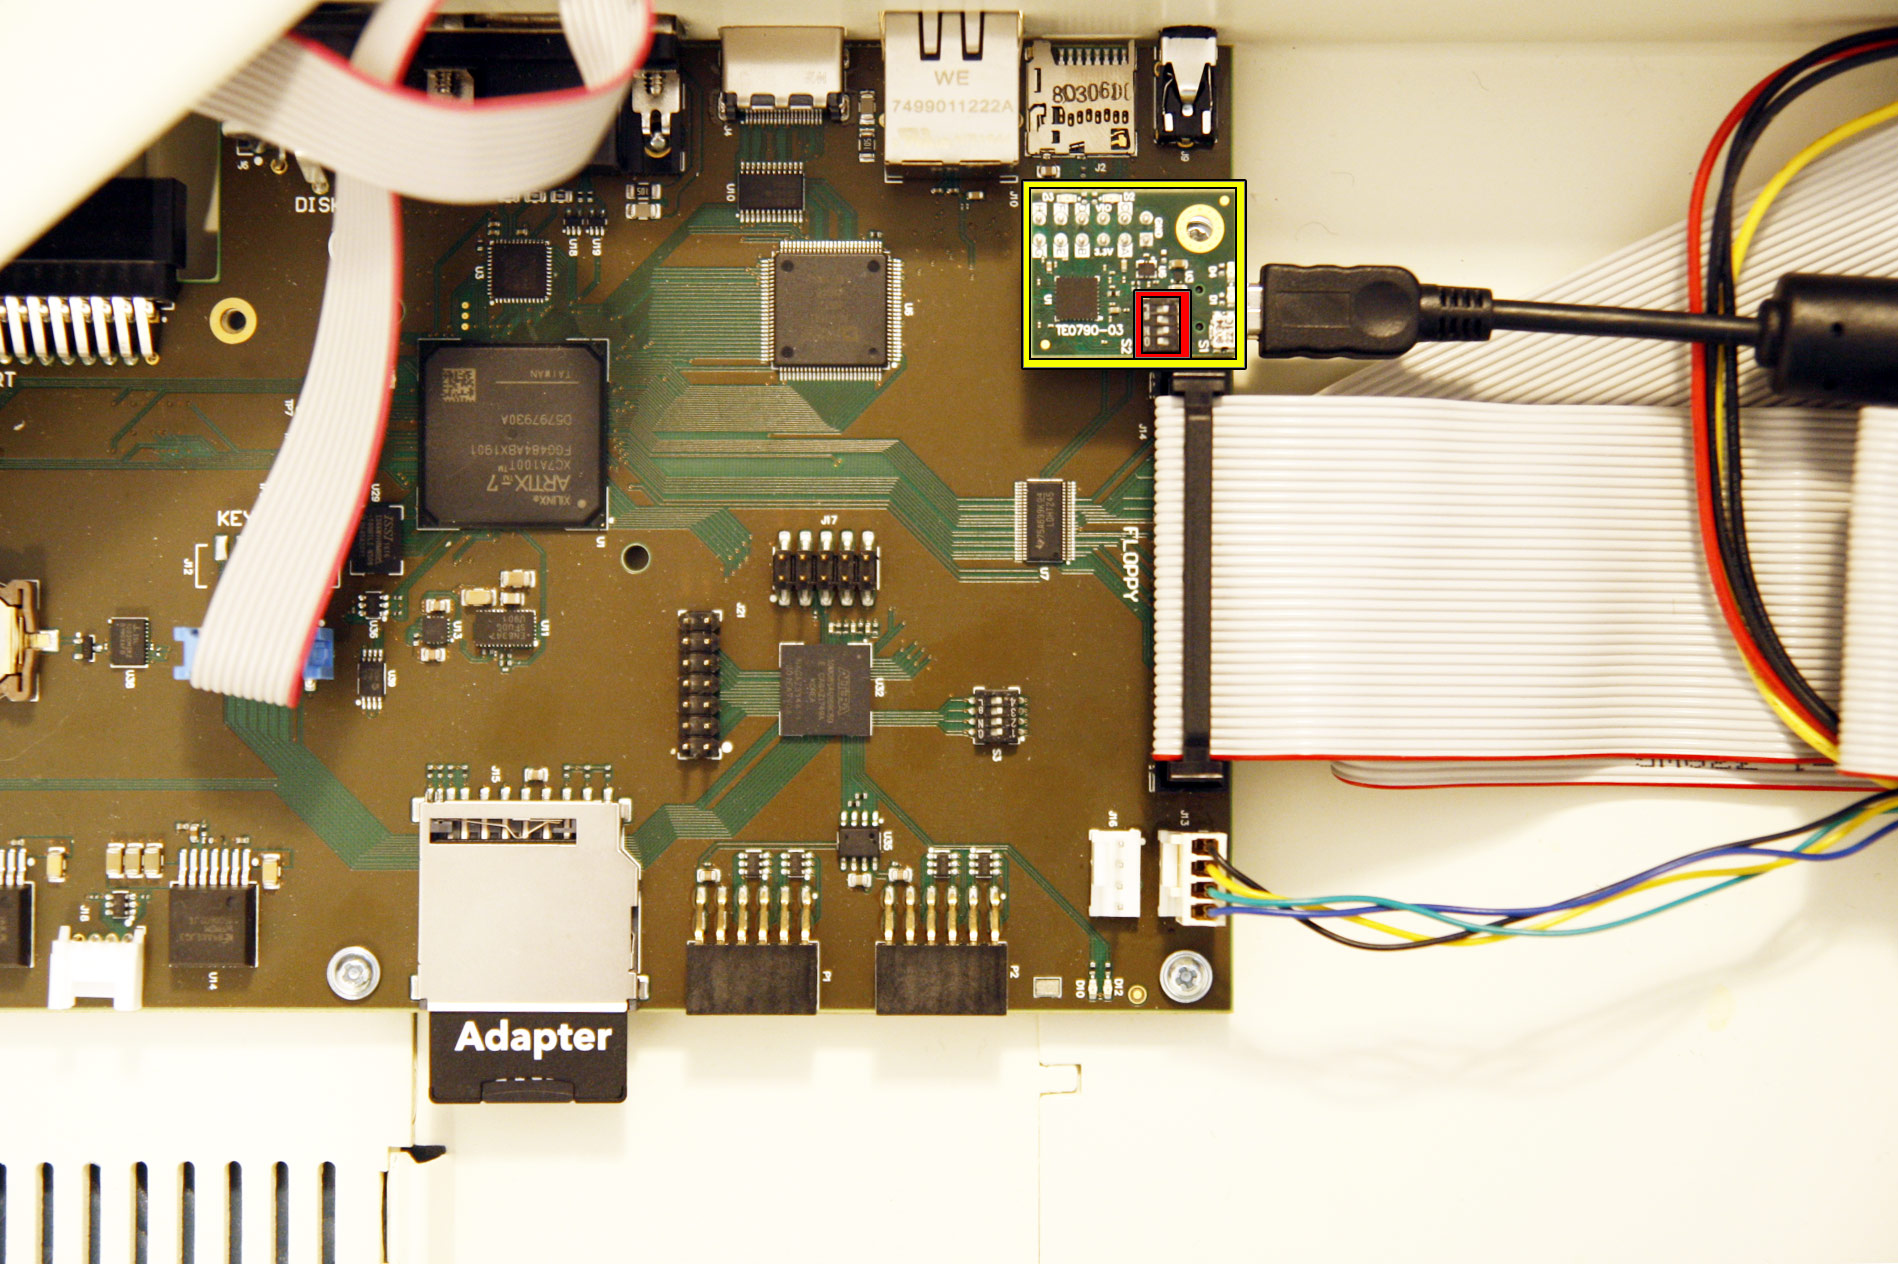
\includegraphics[width=\linewidth]{images/jtag_detail_02.jpg}
\end{tcolorbox}

\begin{tcolorbox}[colback=white,coltext=black]
\underline{Voor eigenaren van een Nexys4-bord}: \\
\\
  Sluit uw micro-USB-kabel aan tussen uw Nexys4-bord en uw pc via de poort met het label ``PROG UART'' (J6), zoals getoond: \\
\\
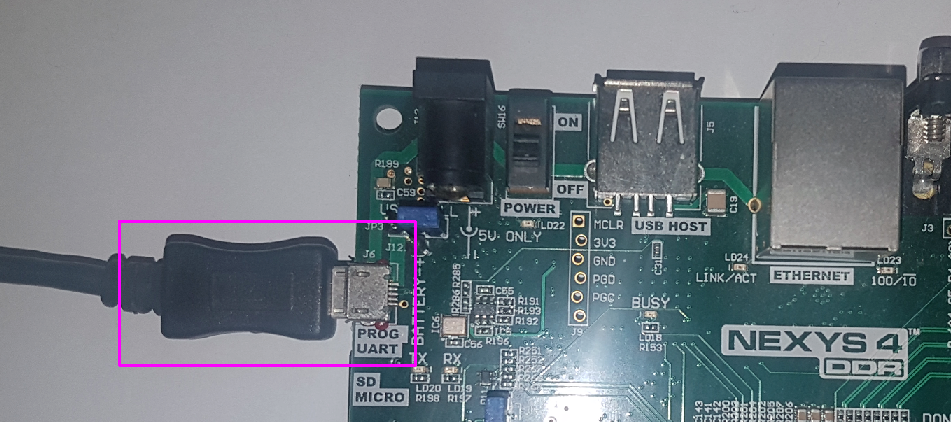
\includegraphics[width=\linewidth]{images/nexys4_comms.png}
\\
\\
Zet bovendien de J1-jumper op de QSPI-stand:
\\
\begin{center}
  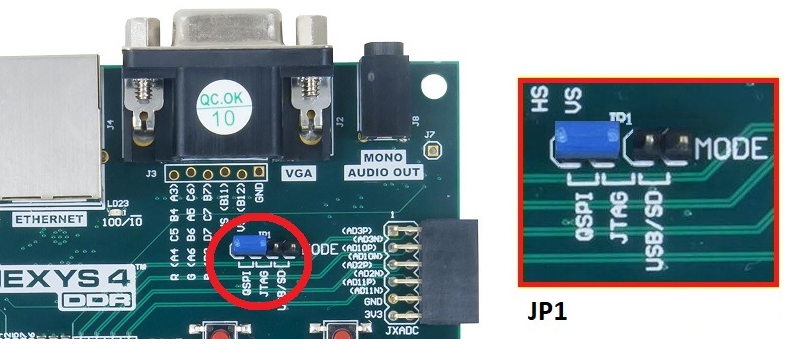
\includegraphics[width=0.8\linewidth]{images/nexys4_j2.png}
\end{center}

\end{tcolorbox}

\begin{itemize}
  \item Sluit uw niet-8-bit computer aan op het FPGA-programmeerapparaat met behulp van de juiste USB-kabel.  \item Schakel de MEGA65-computer in.  \item Open Vivado.
\end{itemize}


\begin{minipage}{\linewidth}
  Stap 1a: Maak een nieuw Vivado-project aan via ``File'', ``Project'', ``New...''. \\  LET OP: Bij toekomstige gelegenheden waarop u de QSPI moet flashen, heropent u dit project (het is niet nodig elke keer een nieuw project aan te maken).  \\
  \begin{center}
    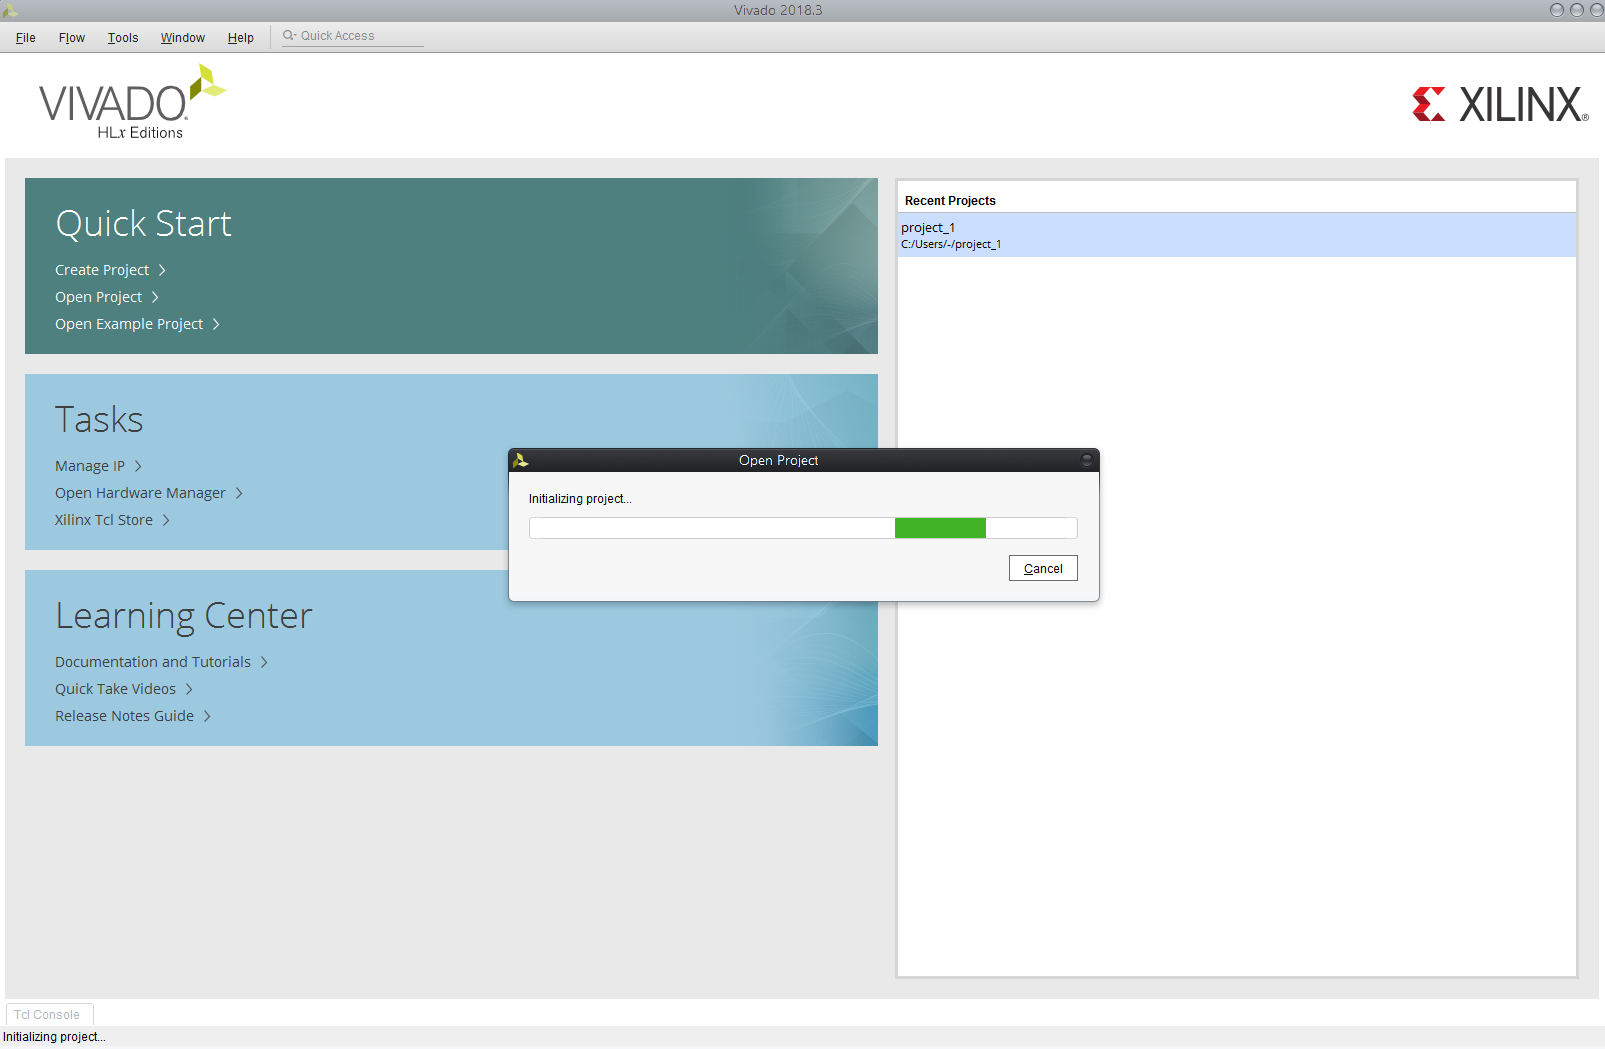
\includegraphics[width=0.8\linewidth]{images/vivado01.png}
  \end{center}
\end{minipage}

\vspace{5mm}

\begin{minipage}{\linewidth}
  Stap 1b: De wizard ``New Project'' verschijnt. Klik op ``Next'': \\
  \begin{center}
    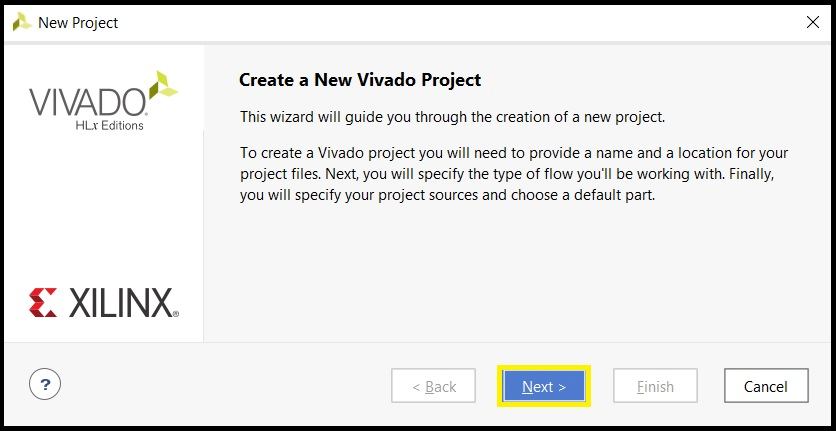
\includegraphics[width=0.8\linewidth]{images/vivado01b.png}
  \end{center}
\end{minipage}

\begin{minipage}{\linewidth}
  Stap 1c: Geef uw project een naam en kies de gewenste locatie en klik op ``Next'':\\
  \begin{center}
    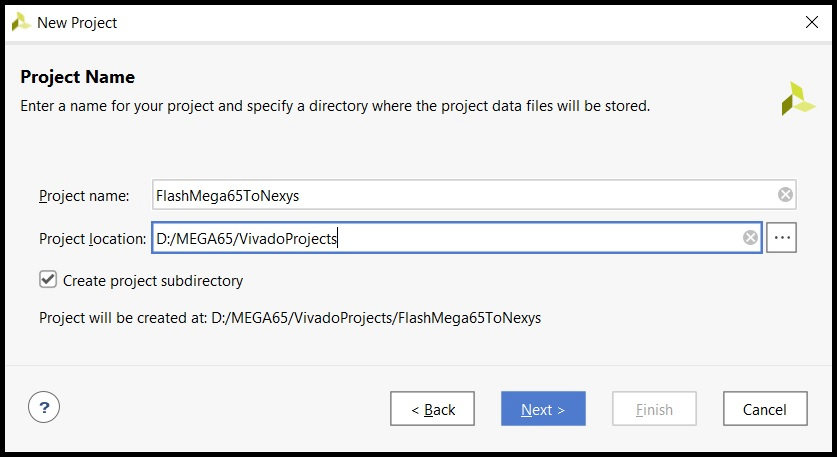
\includegraphics[width=0.8\linewidth]{images/vivado01c.png}
  \end{center}
\end{minipage}

\vspace{5mm}

\begin{minipage}{\linewidth}
  Stap 1d: Laat de standaard geselecteerde opties behouden en klik op ``Next'': \\
  \begin{center}
    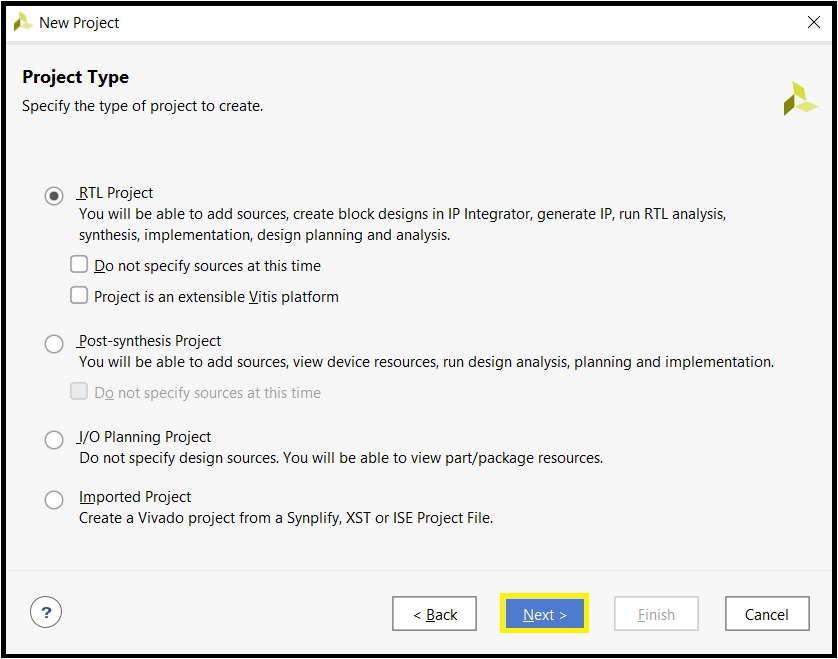
\includegraphics[width=0.8\linewidth]{images/vivado01d.png}
  \end{center}
\end{minipage}

\begin{minipage}{\linewidth}
  Stap 1e: Voeg geen bronnen toe, laat de standaard geselecteerde opties behouden en klik op ``Next'': \\
  \begin{center}
    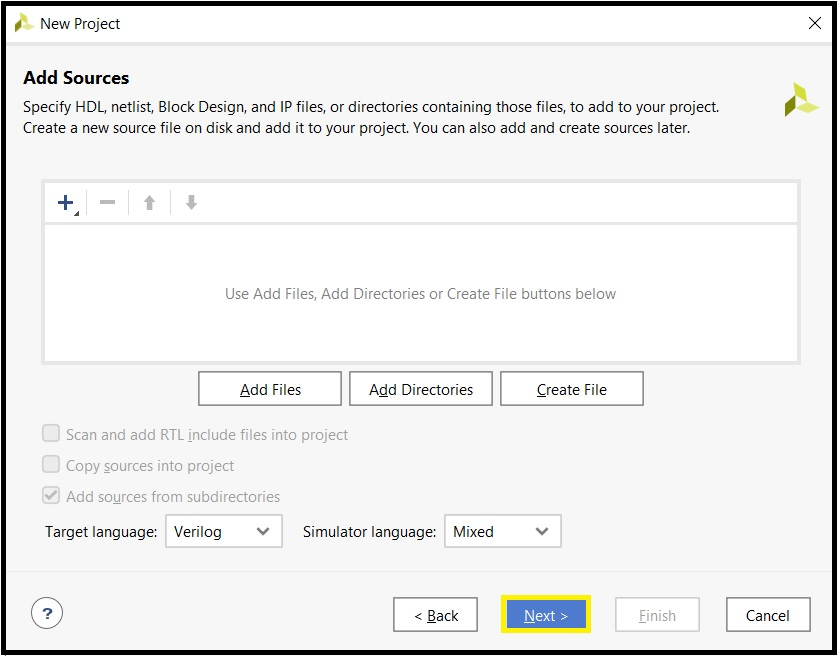
\includegraphics[width=0.7\linewidth]{images/vivado01e.png}
  \end{center}
\end{minipage}

\vspace{5mm}

\begin{minipage}{\linewidth}
  Stap 1f: Laat de standaard geselecteerde opties behouden en klik op ``Next'': \\
  \begin{center}
    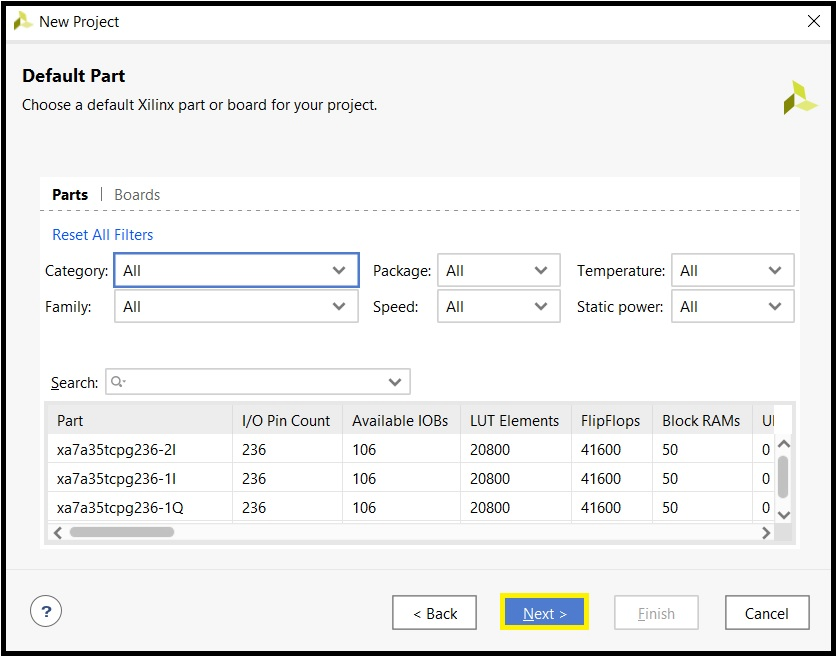
\includegraphics[width=0.7\linewidth]{images/vivado01f.png}
  \end{center}
\end{minipage}

\begin{minipage}{\linewidth}
  Stap 1g: Klik op ``Finish'': \\
  \begin{center}
    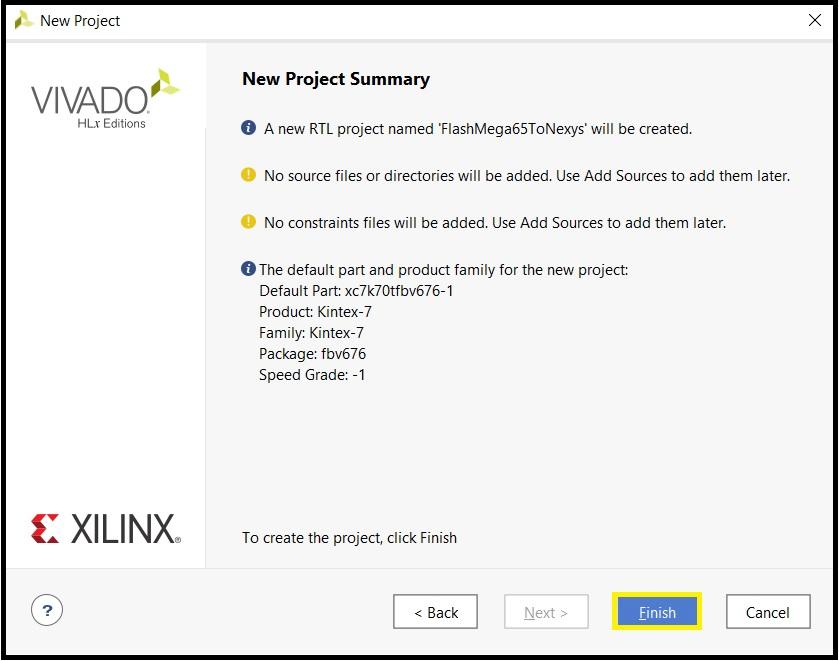
\includegraphics[width=0.8\linewidth]{images/vivado01g.png}
  \end{center}
\end{minipage}

\vspace{5mm}

\begin{minipage}{\linewidth}
  Stap 2: Selecteer in de linker kolom ``Open Hardware Manager'' helemaal onderaan.
  \\
  \begin{center}
    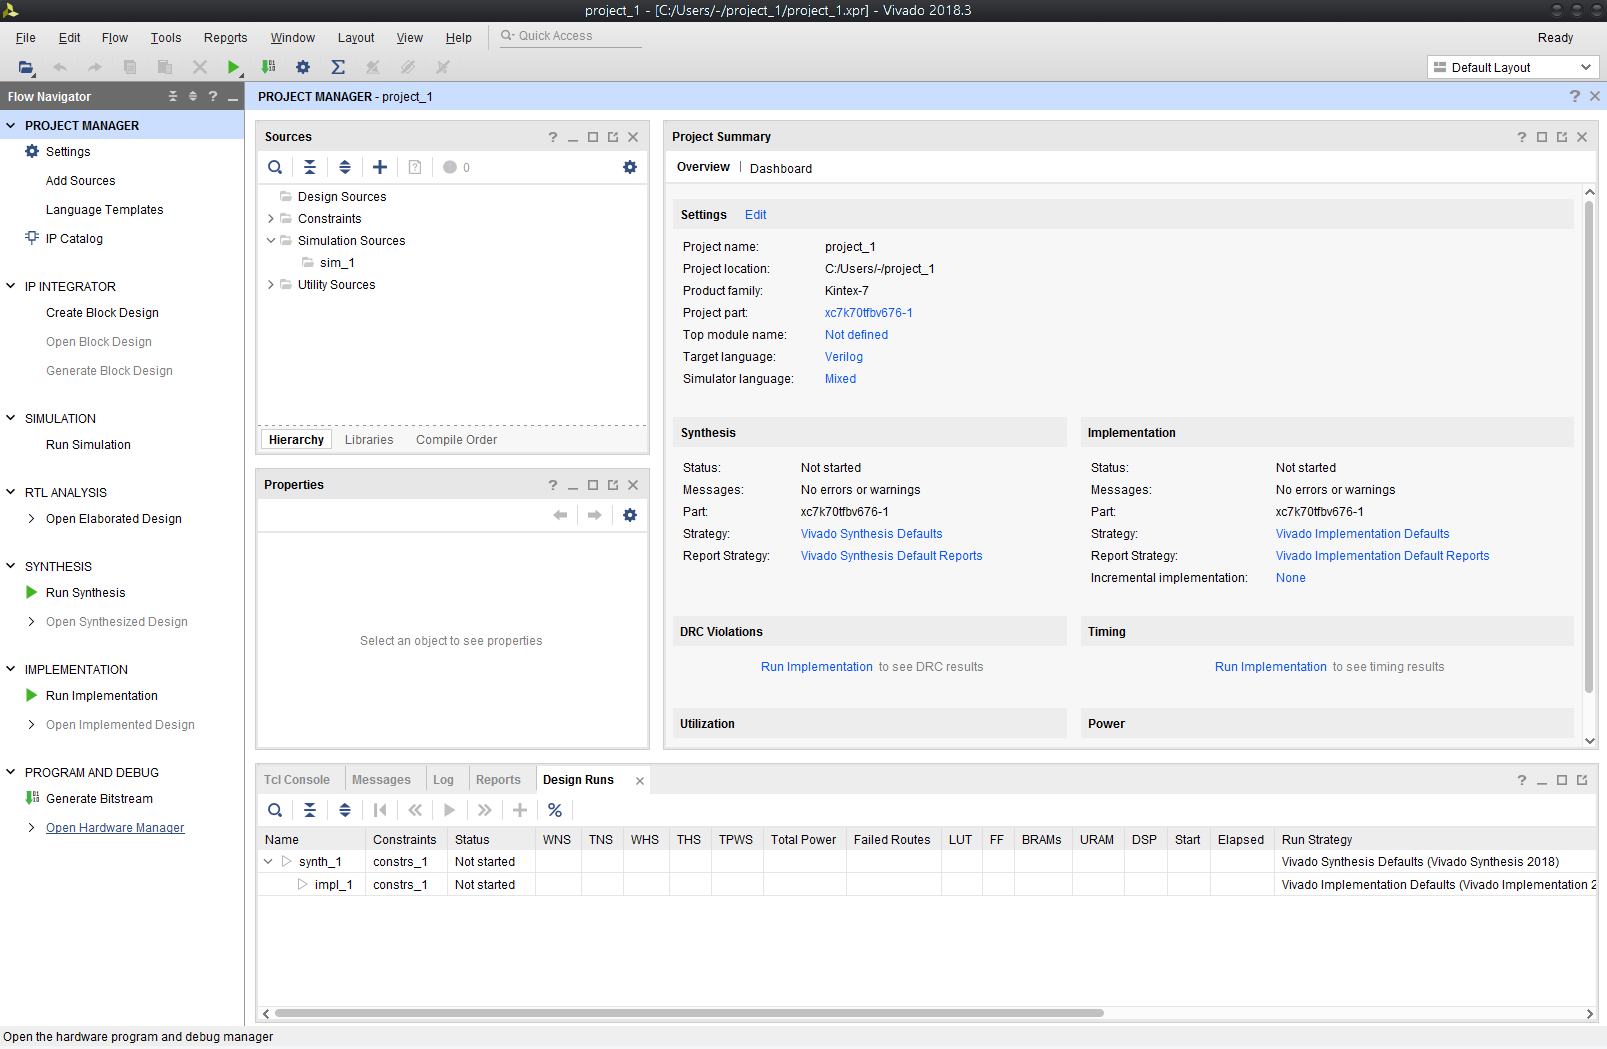
\includegraphics[width=0.8\linewidth]{images/vivado02.png}
  \end{center}
\end{minipage}


\begin{minipage}{\linewidth}
  Stap 3: Verbind met de FPGA: \\  Onder ``Open Hardware Manager'' kiest u ``Open Target'' en vervolgens ``Auto Connect''.
  \\
  \begin{center}
    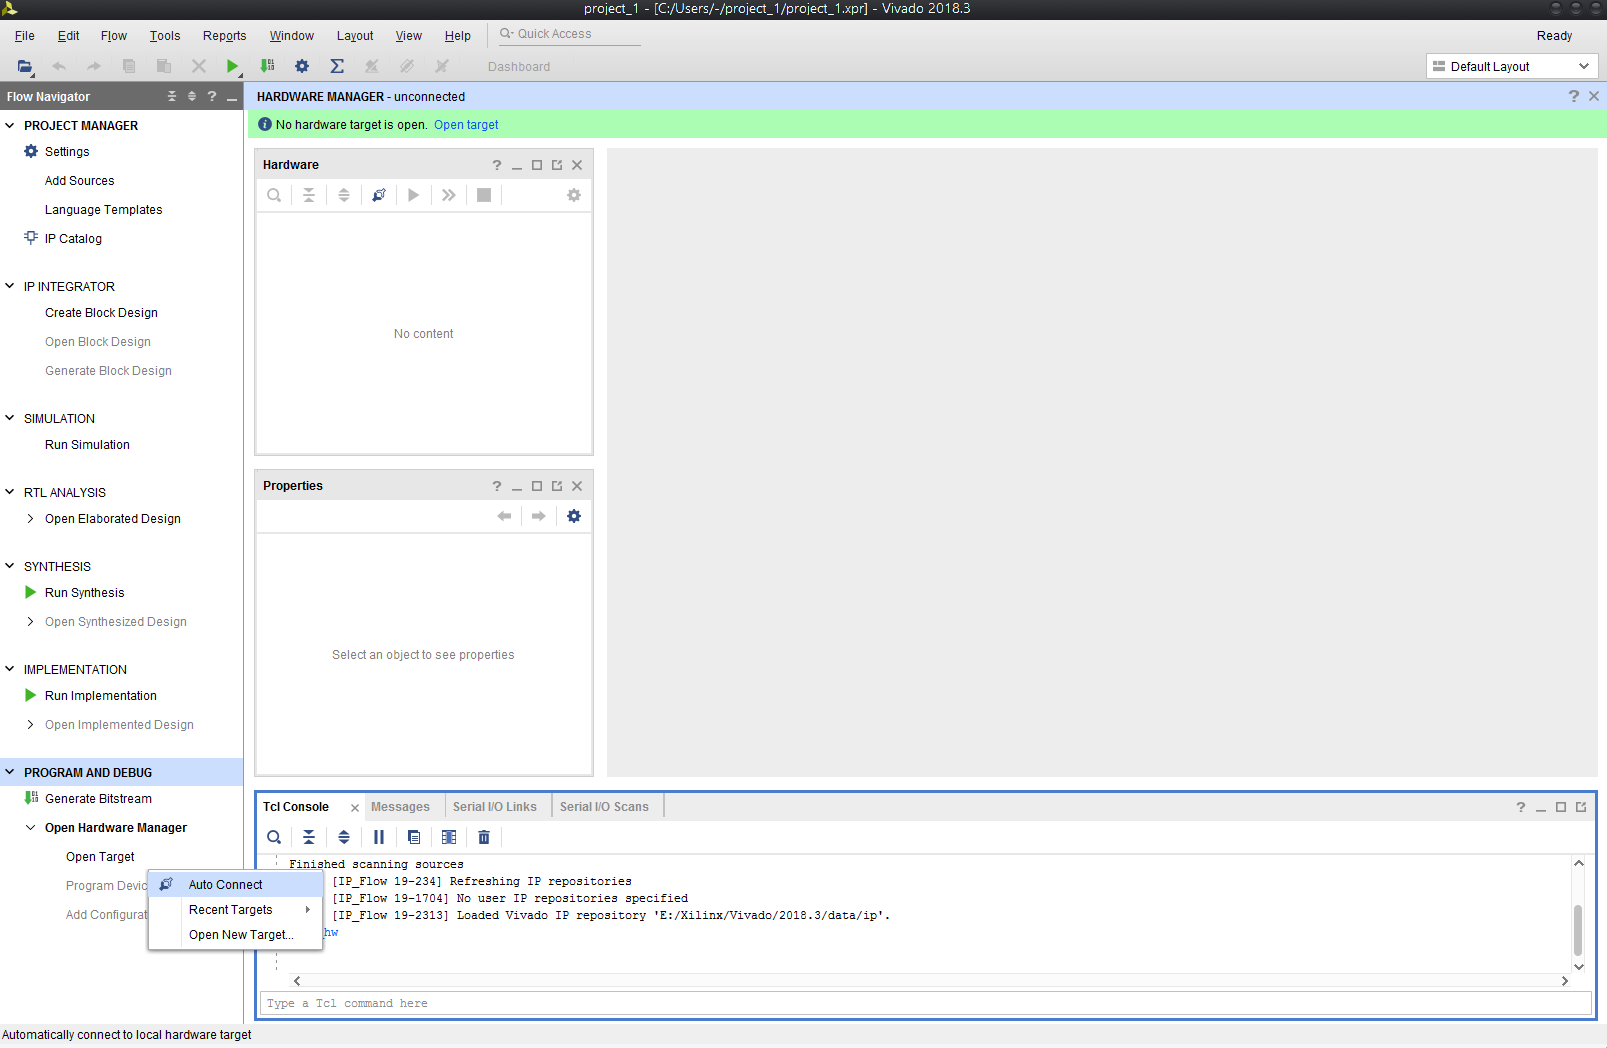
\includegraphics[width=0.8\linewidth]{images/vivado03.png}
  \end{center}
\end{minipage}

\vspace{5mm}

\begin{minipage}{\linewidth}
  Stap 4: Wacht even; ``Connecting to server...'' zou automatisch moeten sluiten zonder een foutmelding aan de console te geven.
  \\
  \begin{center}
    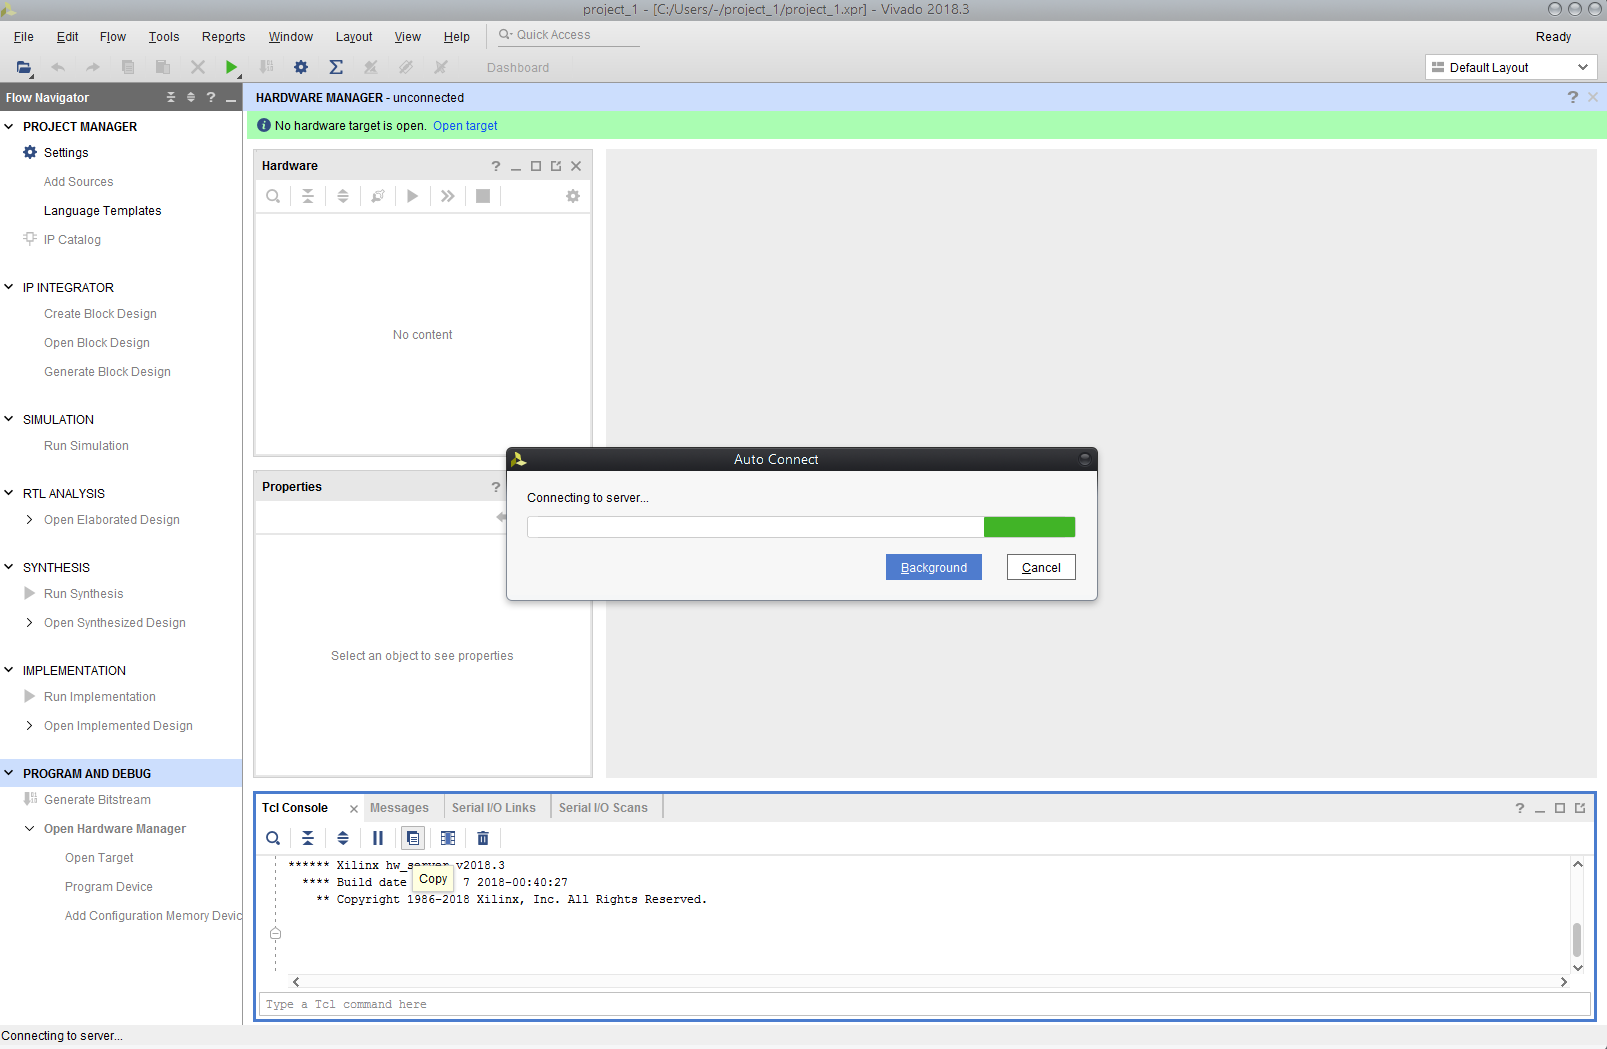
\includegraphics[width=0.8\linewidth]{images/vivado04.png}
  \end{center}
\end{minipage}


\begin{minipage}{\linewidth}
  Stap 5: Onder ``Open Hardware Manager'' kiest u ``Add Configuration Memory Device'' en vervolgens:
  \begin{itemize}
    \item \underline{Voor MEGA65R3/R3A/R4}: ``xc7a200t\_0''    \item \underline{Voor Nexys4 en MEGA65R2}: ``xc7a100t\_0''.
  \end{itemize}

  \begin{center}
    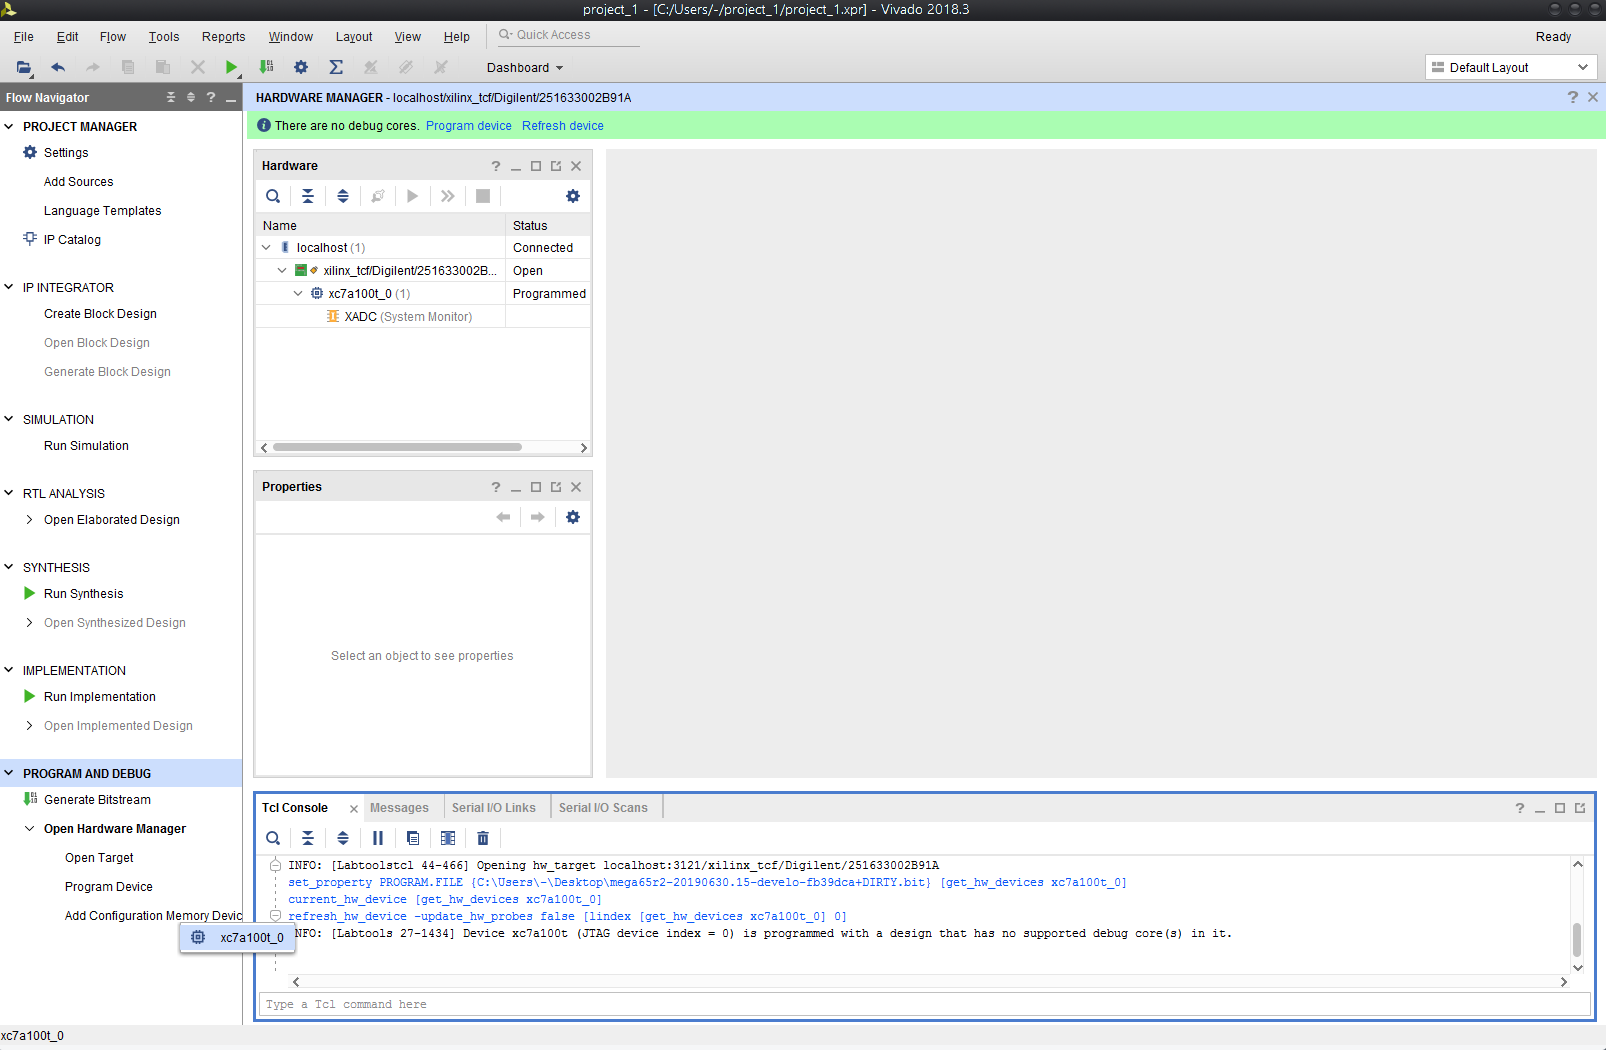
\includegraphics[width=0.7\linewidth]{images/vivado05.png}
  \end{center}
\end{minipage}

\vspace{5mm}

\begin{minipage}{\linewidth}
  Stap 6a: Selecteer Memory Part: \\
  \\
  In het nieuw geopende dialoogvenster:
  \begin{itemize}
    \item \underline{Voor MEGA65R2/R3}: typ ``S25fl256s''    (zonder aanhalingstekens), selecteer vervolgens ``s25fl256sxxxxxxx0-spi-x1\_x2\_x4''    (de bovenste) en klik op ``OK''.    \item \underline{Voor MEGA65R3A/R4}: Vivado kan het grotere flashgeheugen op deze borden niet flashen. Gebruik het flashmenu op de MEGA65.    \item \underline{Voor Nexys4}: typ ``S25fl128s''    (zonder aanhalingstekens), selecteer vervolgens ``s25fl128sxxxxxxx0-spi-x1\_x2\_x4''    (de bovenste) en klik op ``OK''.
  \end{itemize}

  \begin{center}
    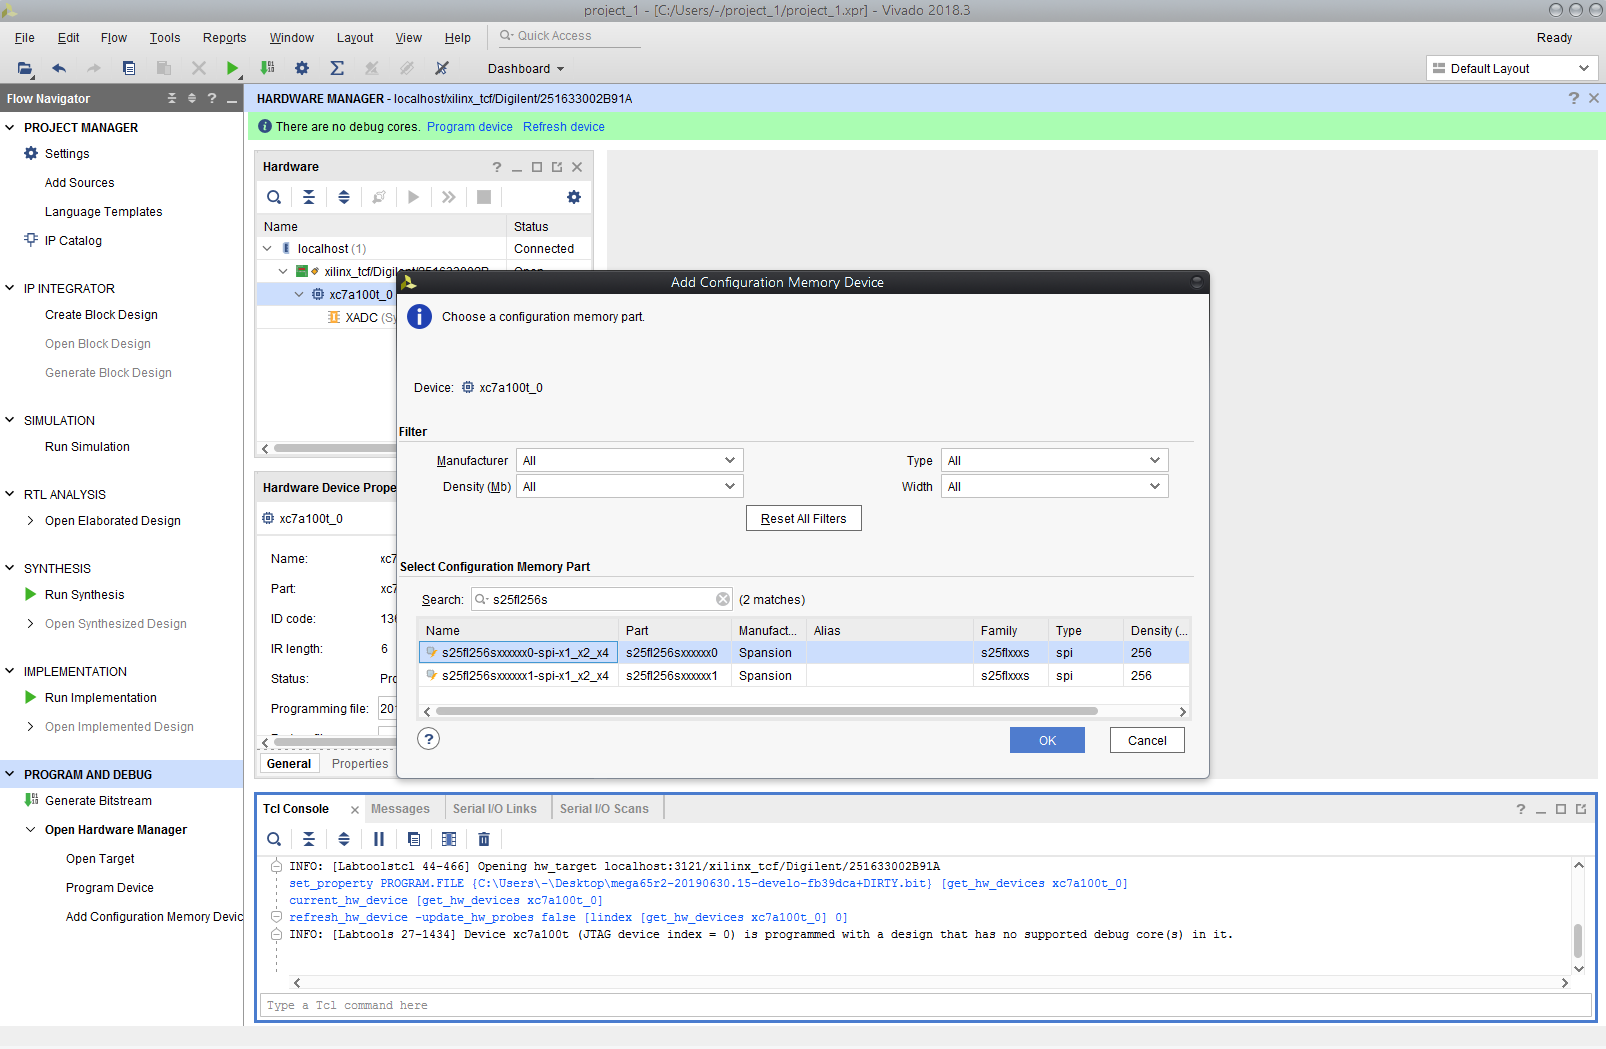
\includegraphics[width=0.7\linewidth]{images/vivado06.png}
  \end{center}
\end{minipage}

\begin{minipage}{\linewidth}
  Stap 6b: Klik op ``OK'' om te bevestigen dat u het configuratiegeheugenapparaat nu wilt programmeren.
  \begin{center}
    \includegraphics[width=0.85\linewidth]{images/vivado06b.png}
  \end{center}
\end{minipage}

\begin{minipage}{\linewidth}
  Stap 6c: Als u zo'n pop-up niet ziet of de QSPI op een later tijdstip opnieuw wilt programmeren, klikt u in het ``Hardware''-venster met de rechtermuisknop op de geheugenconfiguratie en selecteert u ``Program Configuration Memory Device'':
  \begin{center}
    \includegraphics[width=0.85\linewidth]{images/vivado06c.png}
  \end{center}
\end{minipage}

\begin{minipage}{\linewidth}
  Stap 7: Stel de programmeeropties in: \\  Stel in het volgende dialoogvenster ``Configuration file'' in op het pad van uw ``.mcs''-bitstream-bestand. U kunt optioneel ook het ``PRM file''-veld instellen op het pad van uw ``.prm''-bestand. Laat alle overige parameters zoals ze zijn (zie onderstaande screenshot).
  \\
  \begin{center}
    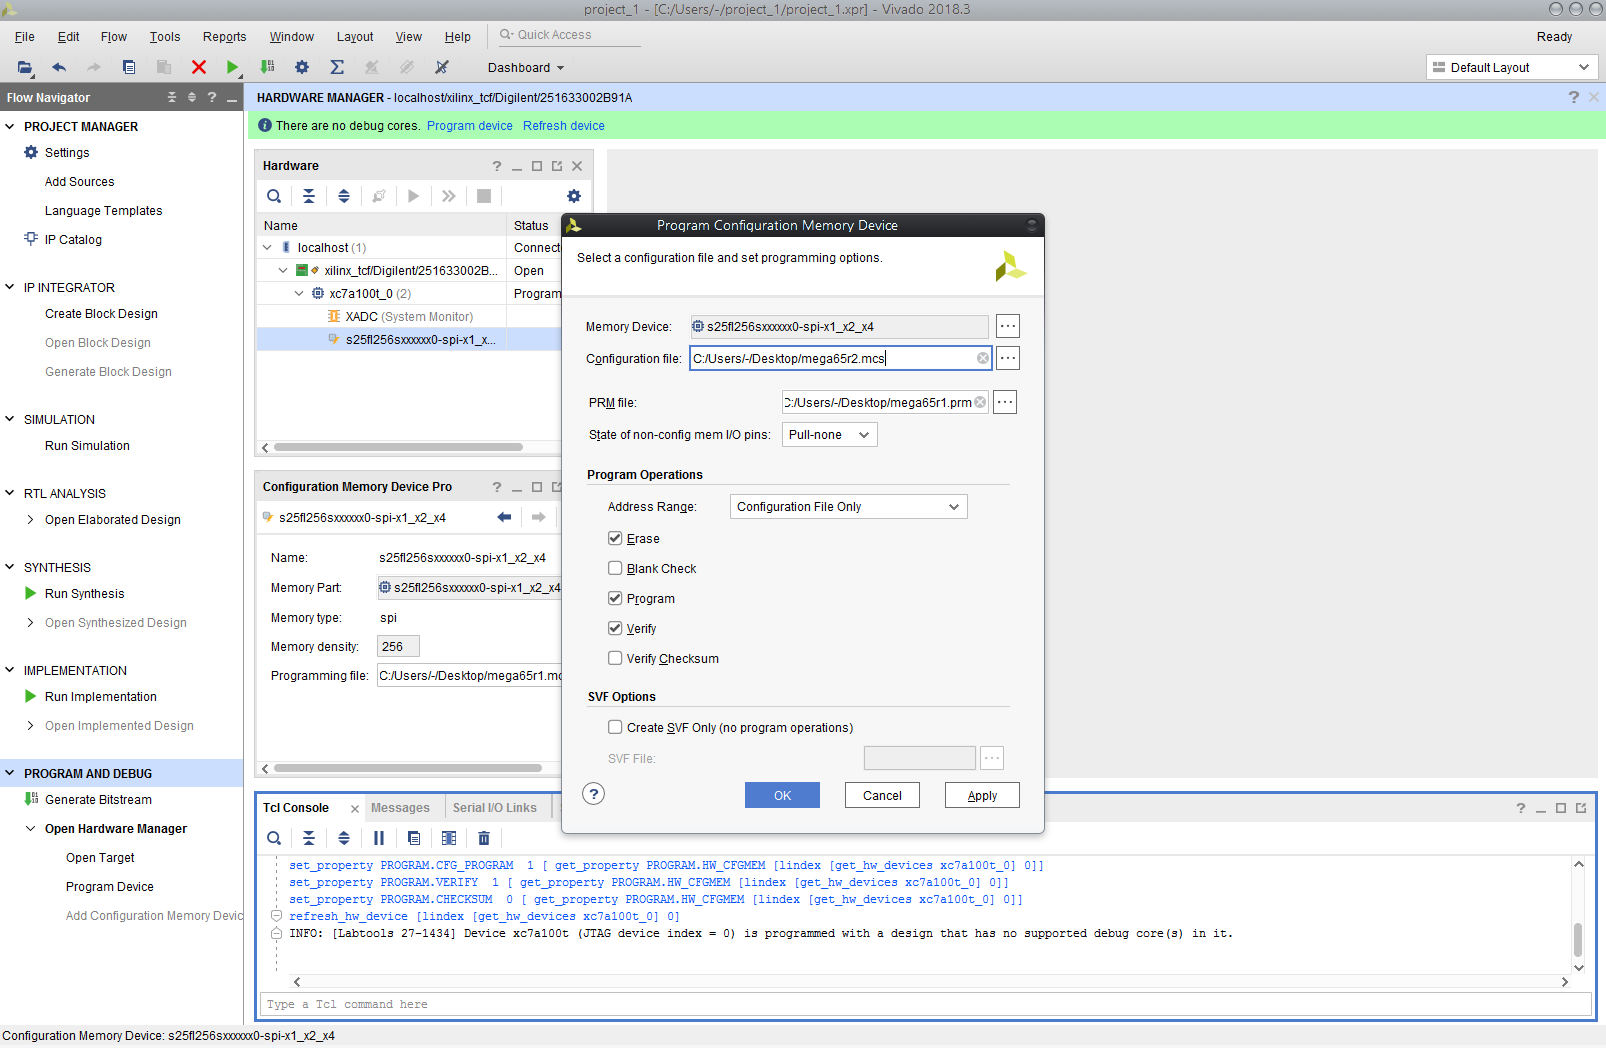
\includegraphics[width=0.85\linewidth]{images/vivado07.png}
  \end{center}
\end{minipage}

\vspace{1mm}

\begin{minipage}{\linewidth}
  Stap 8: Wacht geduldig tot het programmeren is voltooid.  Dit kan enkele minuten duren, omdat de Vivado-software het flashgeheugen dat wordt gebruikt om de FPGA bij het inschakelen te initialiseren, eerst wist en vervolgens opnieuw programmeert.
  \\
  \begin{center}
    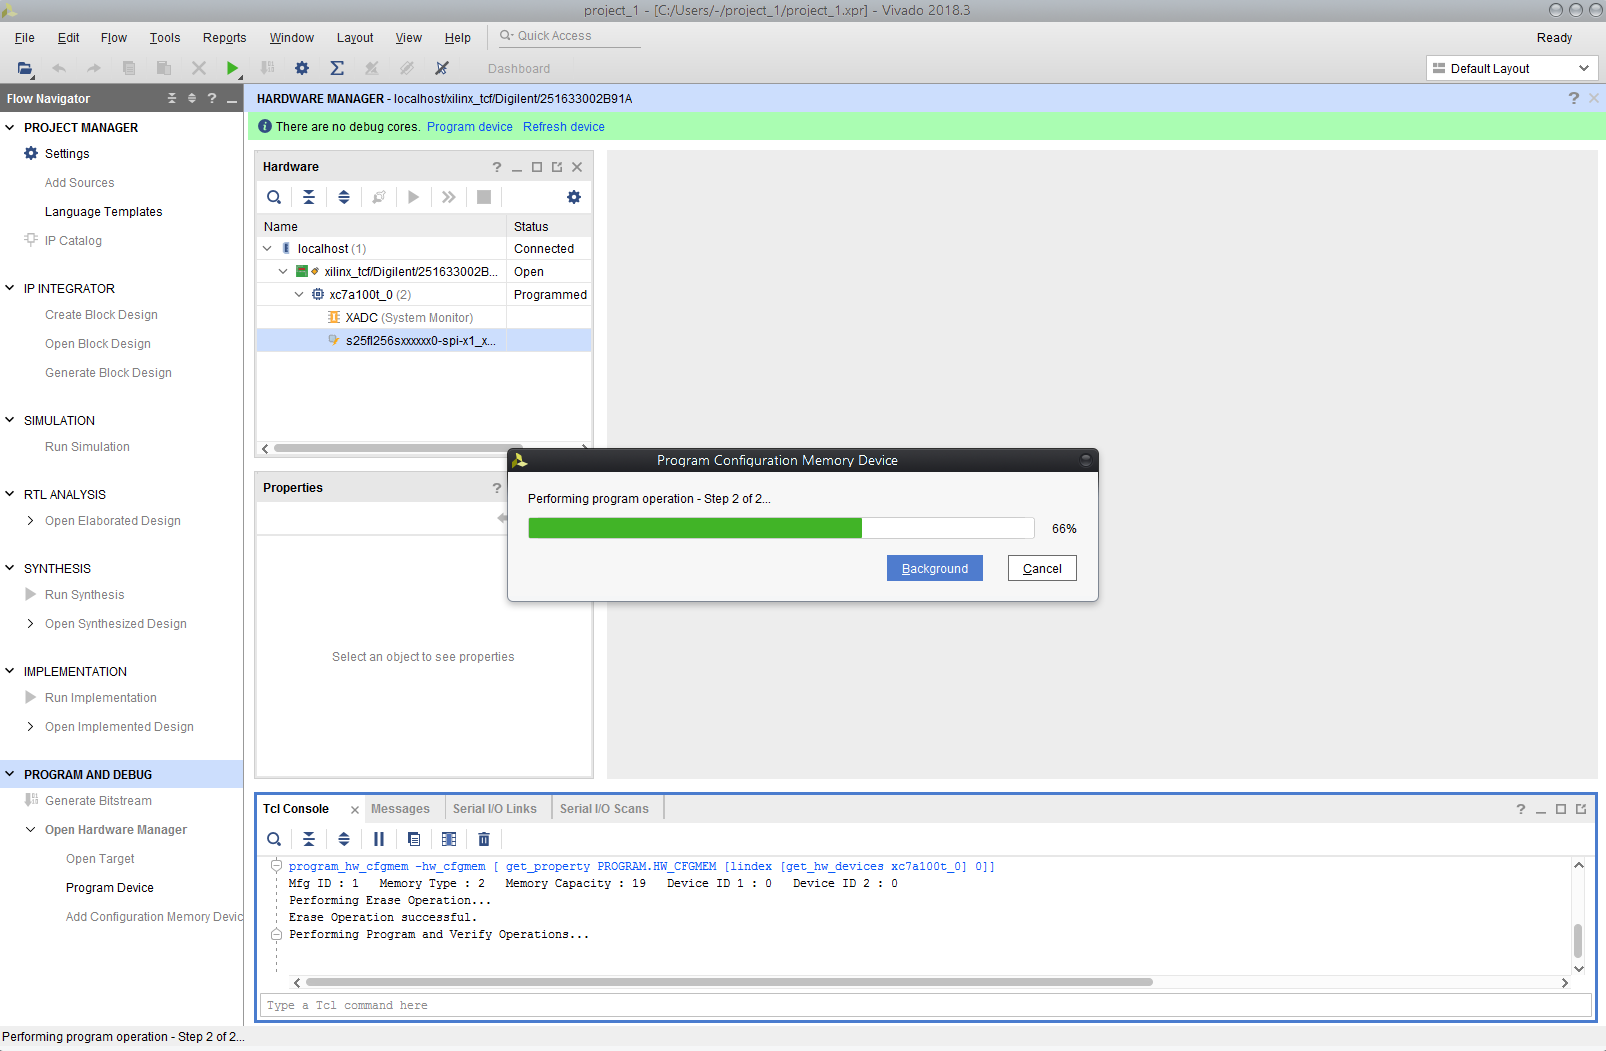
\includegraphics[width=0.85\linewidth]{images/vivado08.png}
  \end{center}
\end{minipage}


\begin{minipage}{\linewidth}
Stap 9: Als uw scherm eruitziet als de onderstaande screenshot, is uw nieuwe bitstream succesvol geflasht in Slot 0 van uw QSPI-flashgeheugen!
  \\
  \begin{center}
    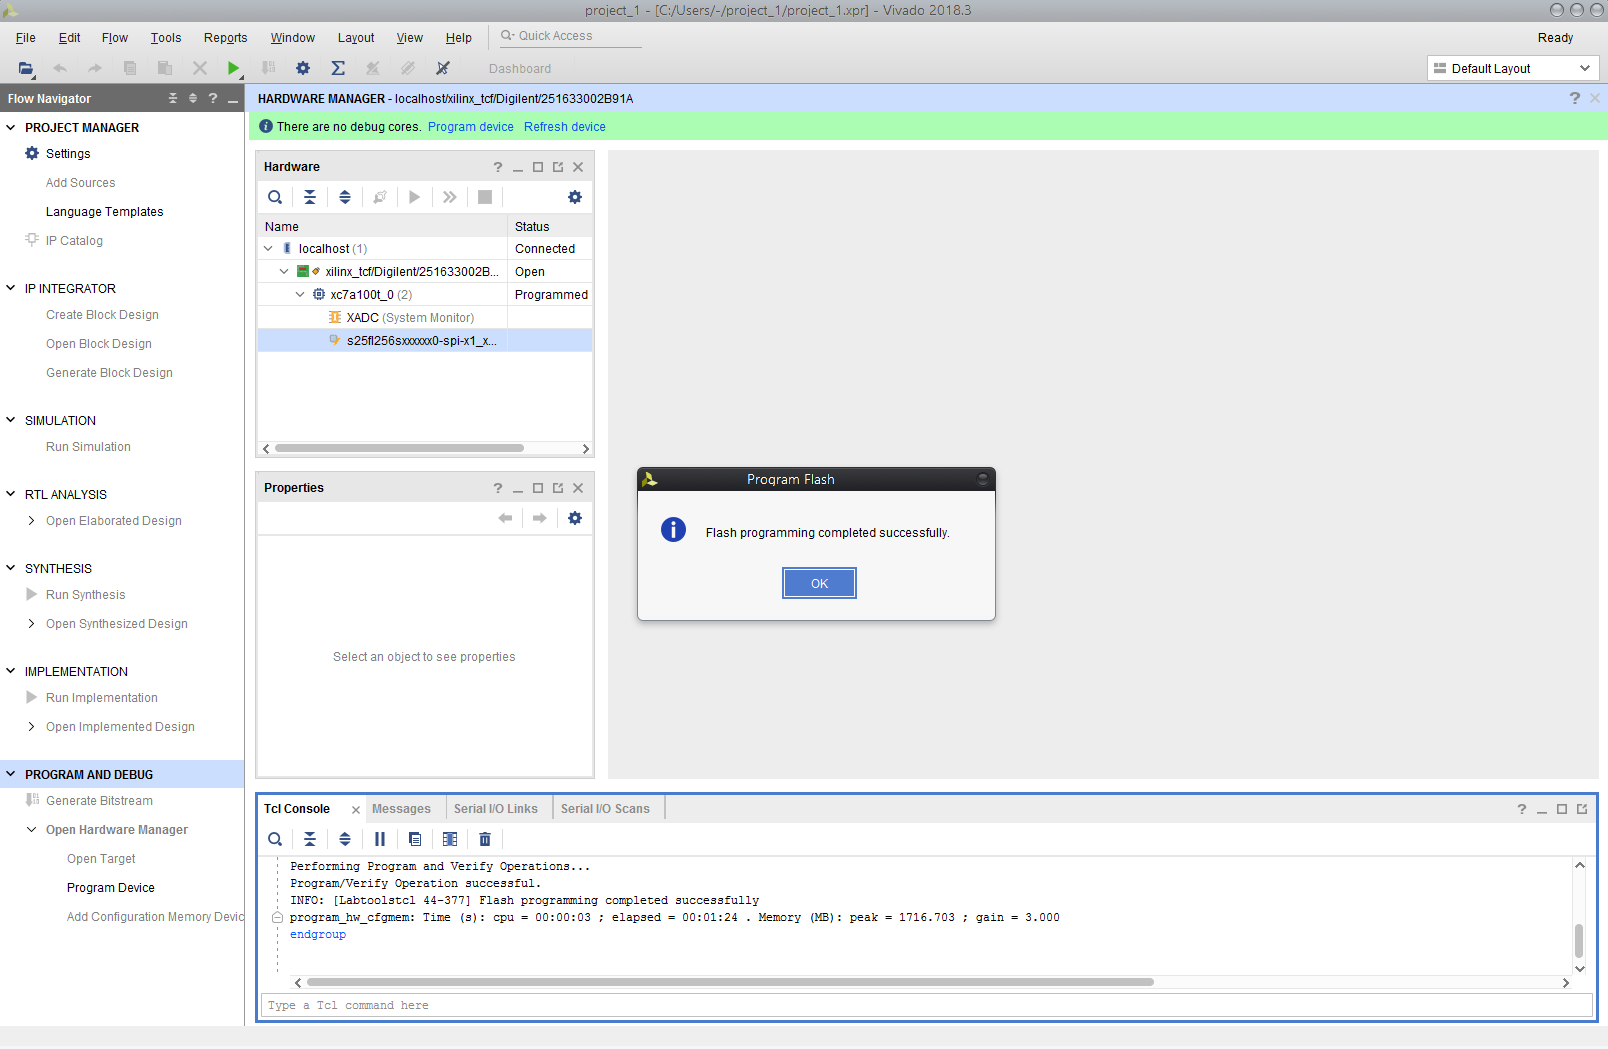
\includegraphics[width=0.8\linewidth]{images/vivado09.png}
  \end{center}
\end{minipage}

\vspace{5mm}

\begin{minipage}{\linewidth}
Stap 10: Als u de FPGA opnieuw wilt flashen, kan het zijn dat de optie ``Add Configuration Memory Device'' uit stap 5 grijs weergegeven wordt.
Selecteer in dat geval ``s25fl256sxxxxxxx0-spi-x1\_x2\_x4''  in het ``Hardware''-venster, druk op de rechtermuisknop en selecteer ``Program Configuration Memory Device'' om te flashen.
  \\
  \begin{center}
    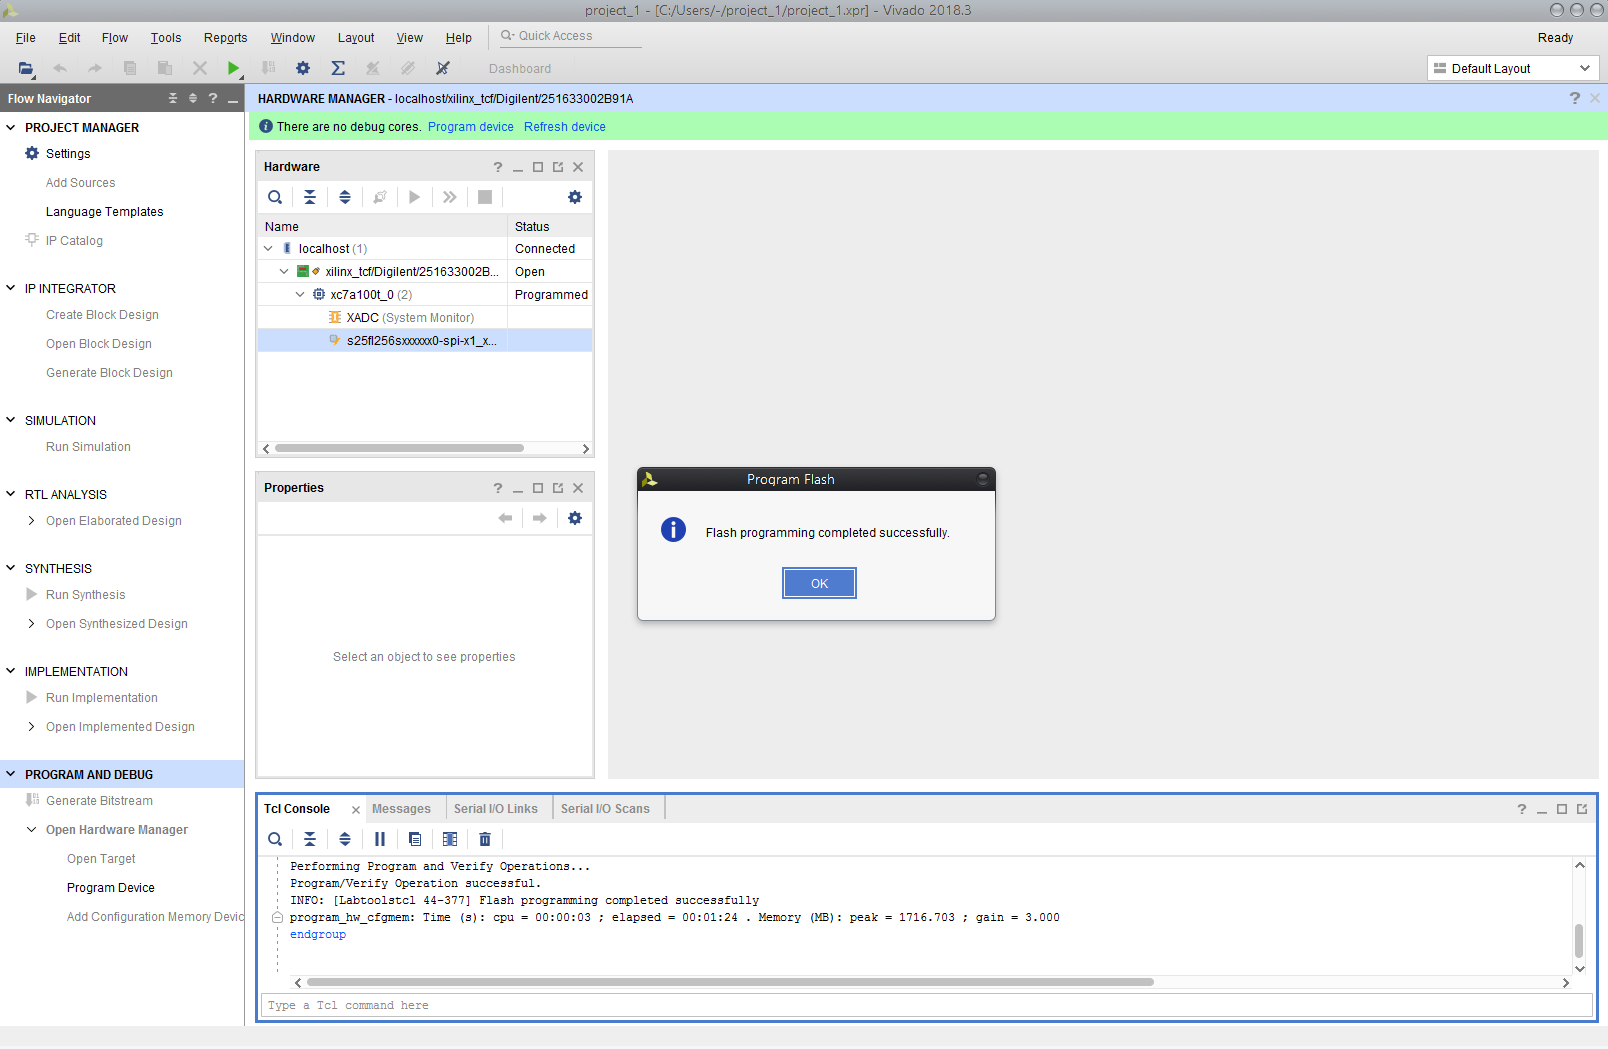
\includegraphics[width=0.8\linewidth]{images/vivado09.png}
  \end{center}
\end{minipage}


\section{De CPLD in het toetsenbord van de MEGA65 flashen met Lattice Diamond}
\label{sec:flashcpld}


Indien u ervoor kiest om door te gaan, heeft u een TE0790-03 JTAG-programmeermodule en een werkende installatie van Lattice Diamond Programmer-software nodig. Dit kan op zowel Windows als Linux, maar in beide gevallen moet u de benodigde USB-stuurprogramma's installeren. Het is ook noodzakelijk dat dip-schakelaars 1 en 3 op de AAN-stand staan en dip-schakelaars 2 en 4 op de UIT-stand op de TE-0790. Met de MEGA65 losgekoppeld van de voeding moet de TE-0790 op de JB1-connector worden geïnstalleerd, die zich tussen de diskettedatakabel en de audiojack bevindt. De vergulde opening van de TE-0790 moet in lijn liggen met het schroefgat eronder. De mini-USB-kabel verbindt zich vervolgens aan de kant richting het 3.5'' diskettestation. De volgende afbeelding toont de juiste positie: de TE0790 is omringd door de gele kast en de dip-schakelaars door de rode kast. Dip-schakelaar 1 is de dichtstbijzijnde bij de diskettedatakabel.


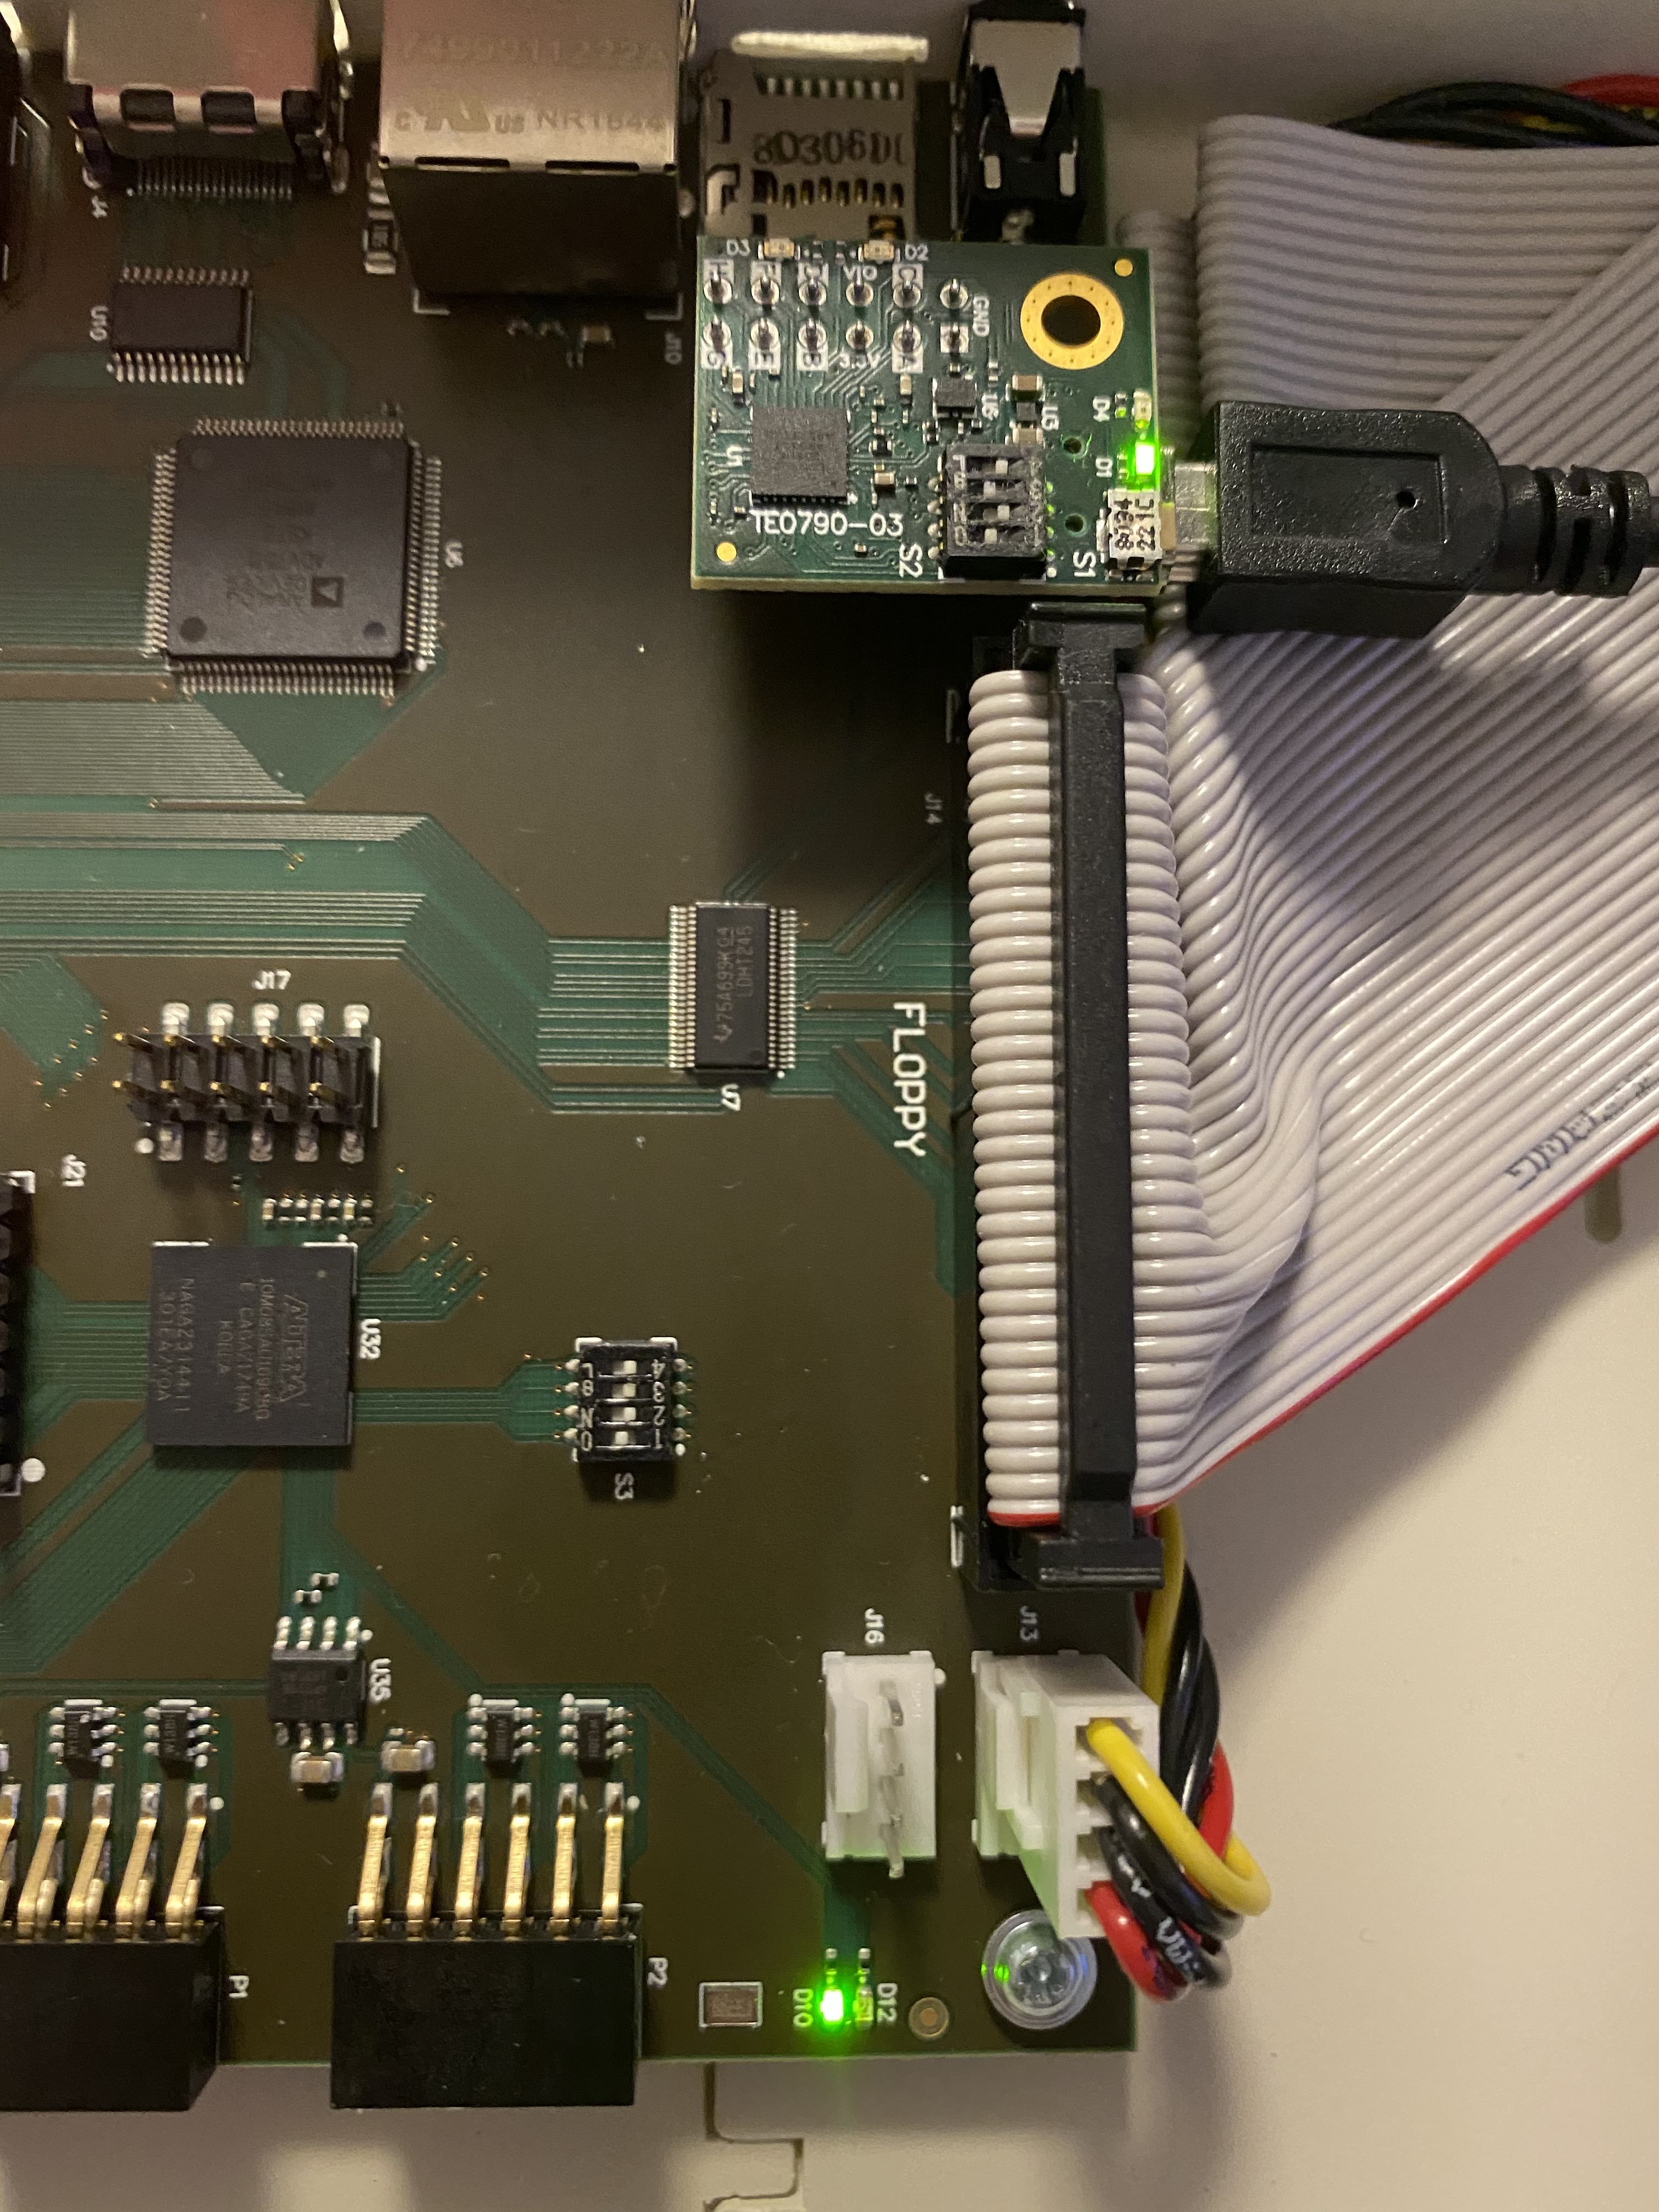
\includegraphics[width=\linewidth]{images/jtag_detail_05.jpg}


Op de PCB van een R2/R3/R3A/R4 MEGA65-moederbord moet dip-schakelaar 1 (de dichtstbijzijnde bij de gebruiker die voor de computer zit) op de AAN-stand staan. De overige schakelaars moeten UIT staan. Het toetsenbord gaat in de ``ambulance-modus'' (blauwe flitsende lichten) wanneer het correct is ingesteld.

Sluit uw niet-8-bit computer aan op het FPGA-programmeerapparaat met behulp van een mini-USB-kabel. Schakel de MEGA65-computer in. Open de Diamond Programmer, die van het internet kan worden gedownload.

\begin{minipage}{\linewidth}
Stap 1: Open DIAMOND PROGRAMMER: \\Selecteer ``Create a new project from a JTAG scan''. Indien het veld onder ``Cable:'' leeg is, klikt u op ``Detect Cable''.
\\
  \begin{center}
  
\includegraphics{images/diamond01.png}
  \end{center}
\end{minipage}

\vspace{5mm}

\begin{minipage}{\linewidth}
Stap 2: Maak een nieuw project aan: \\Indien het dialoogvenster ``Programmer: Multiple Cables Detected'' verschijnt, selecteert u het eerste item (``Location 0000'') en klikt u op ``OK''.
  \begin{center}
  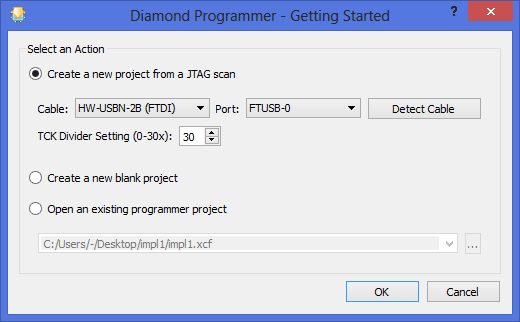
\includegraphics[width=0.7\linewidth]{images/diamond02.png}
  \end{center}
\end{minipage}


\begin{minipage}{\linewidth}
Stap 3: Selecteer kabel: \\U heeft nu een nieuw project aangemaakt dat ``MachXO2'' onder ``Device Family'' en ``LCMXO2-1200HC'' onder ``Device'' zou moeten weergeven.
  \begin{center}
  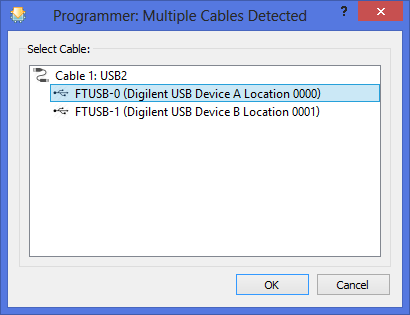
\includegraphics[width=0.6\linewidth]{images/diamond03.png}
  \end{center}
\end{minipage}

\vspace{5mm}

\begin{minipage}{\linewidth}
Stap 4: Nieuw Diamond Programmer-project: \\Kies ``File'' en vervolgens ``Open File'' om het Diamond Programmer-project met de firmware-update voor het MEGA65-toetsenbord te laden.
  \begin{center}
  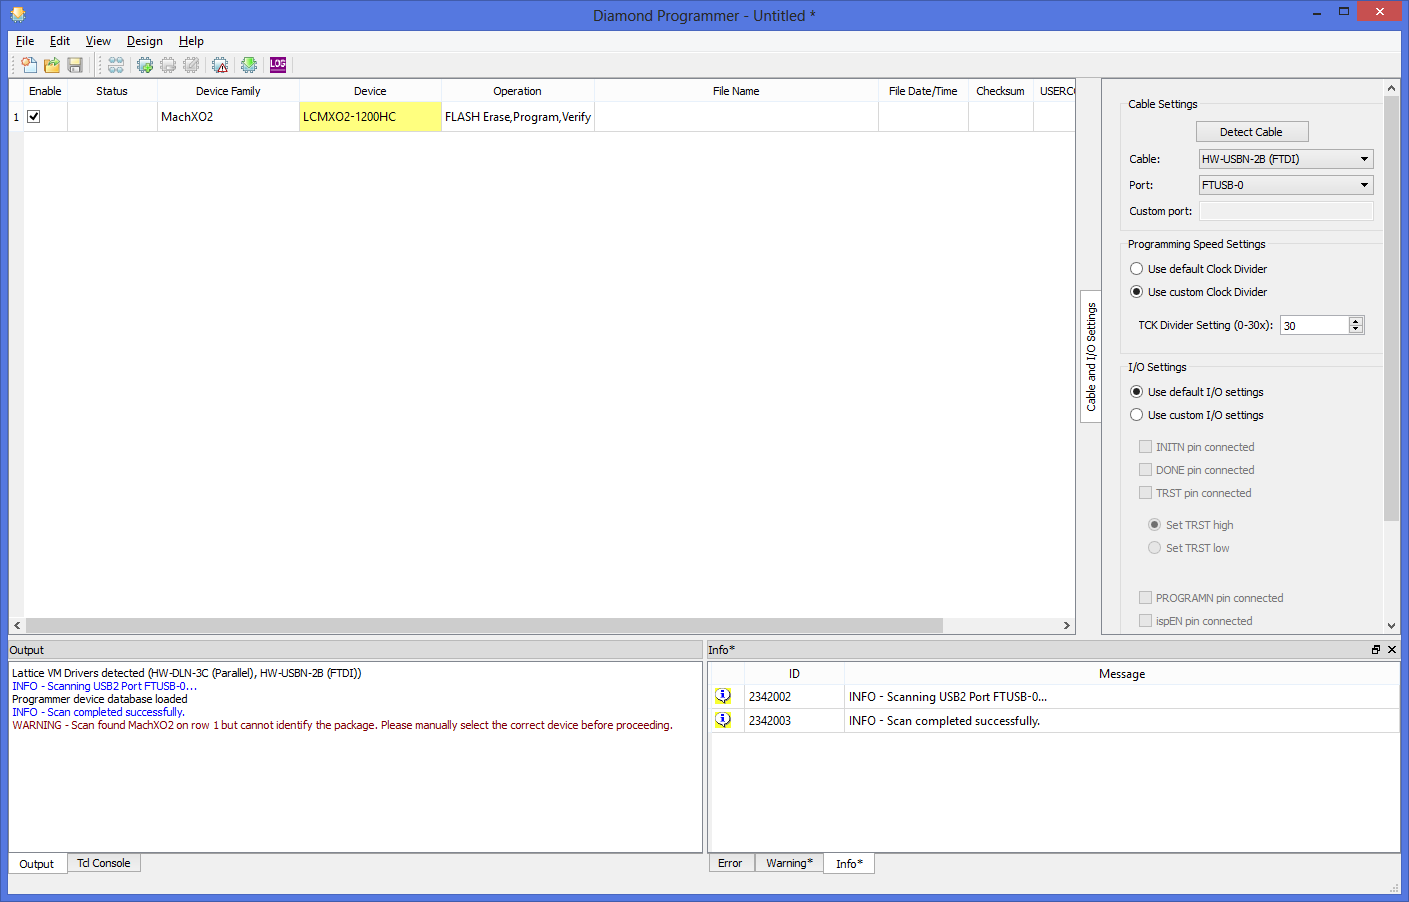
\includegraphics[width=0.8\linewidth]{images/diamond04.png}
  \end{center}
\end{minipage}


\begin{minipage}{\linewidth}
Stap 5: Open project: \\Navigeer naar de map met de uitgepakte firmwarebestanden voor het MEGA65-toetsenbord die u hebt ontvangen en selecteer het bestand met de extensie ``.xcf''.
  \begin{center}
  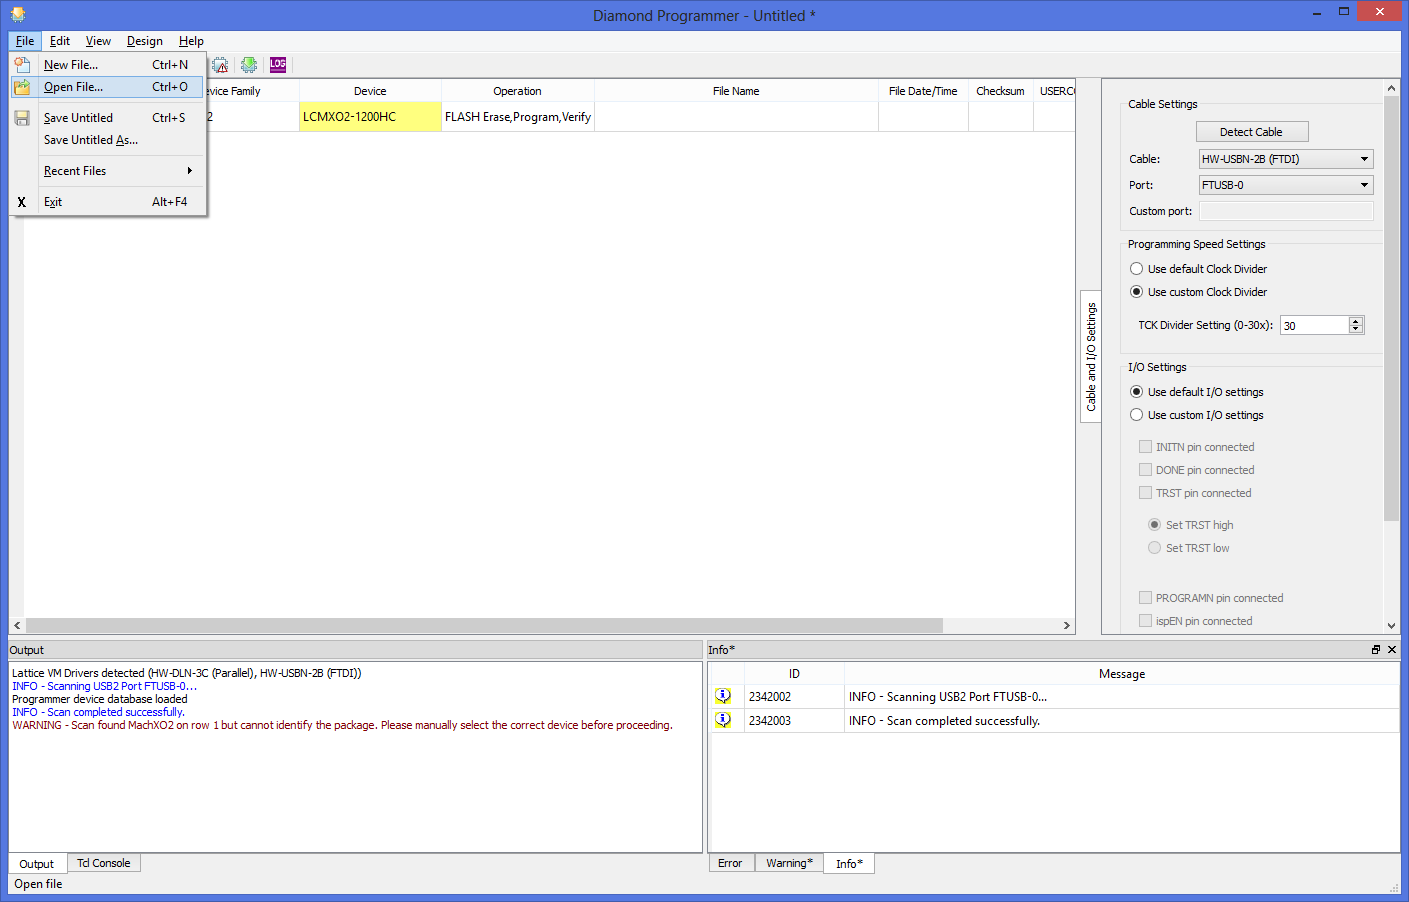
\includegraphics[width=0.8\linewidth]{images/diamond05.png}
  \end{center}
\end{minipage}

\vspace{5mm}

\begin{minipage}{\linewidth}
Stap 6: Selecteer projectbestand: \\Klik op de drie puntjes onder ``File Name'' om het juiste pad in te stellen en het bestand met de extensie ``.jed'' te vinden.
  \begin{center}
  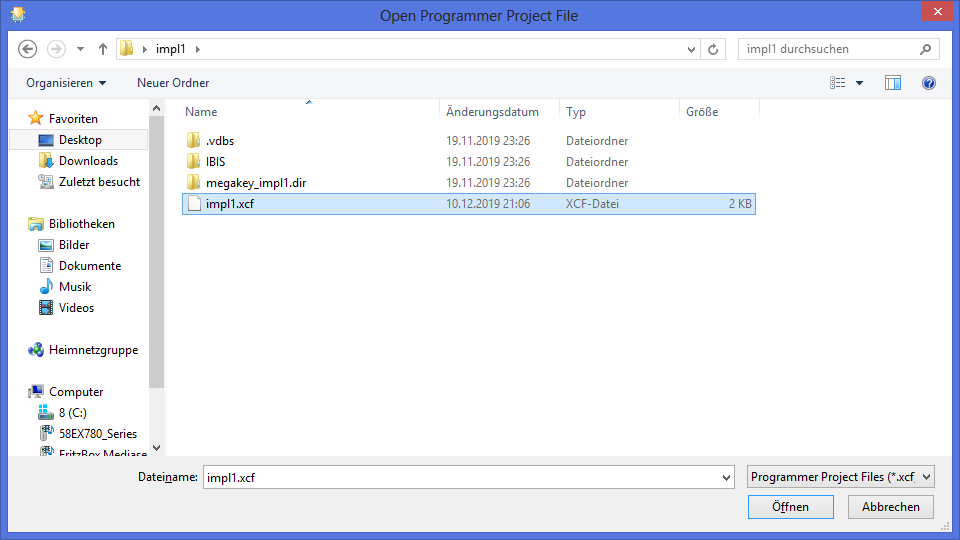
\includegraphics[width=0.8\linewidth]{images/diamond06.png}
  \end{center}
\end{minipage}


\begin{minipage}{\linewidth}
Stap 7: Kies het juiste pad van het .jed-bestand: \\Selecteer het bestand met de extensie ``.jed'' en klik op ``OK''.
  \begin{center}
  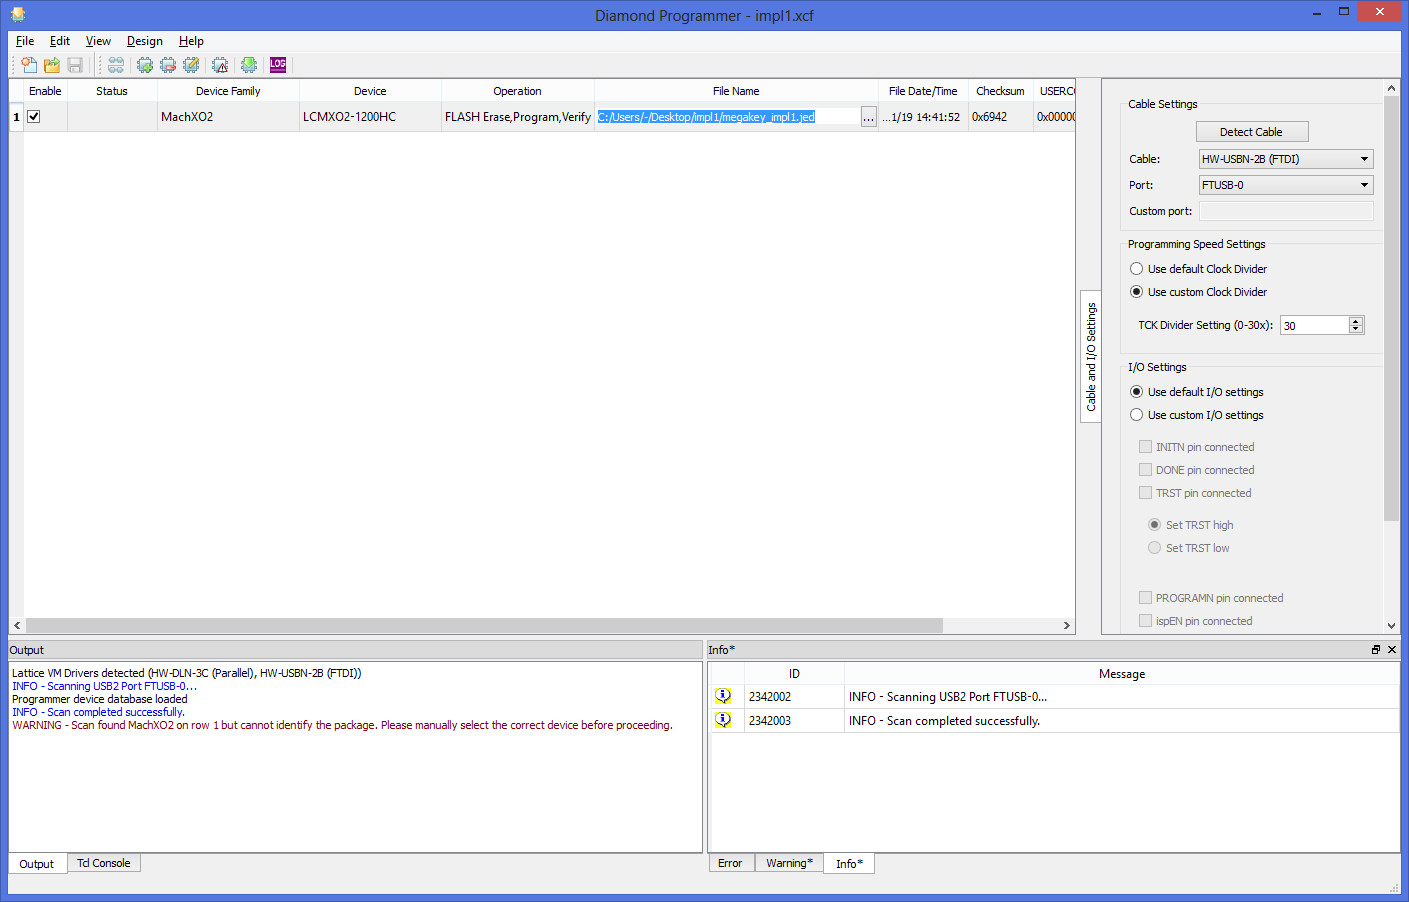
\includegraphics[width=0.8\linewidth]{images/diamond07.png}
  \end{center}
\end{minipage}

\vspace{5mm}

\begin{minipage}{\linewidth}
Stap 8: Selecteer .jed-bestand: \\Klik op het icoon met de groene pijl naar beneden ``PROGRAM'', dat lijkt op het icoon van het Diamond Programmer-programma.
  \begin{center}
  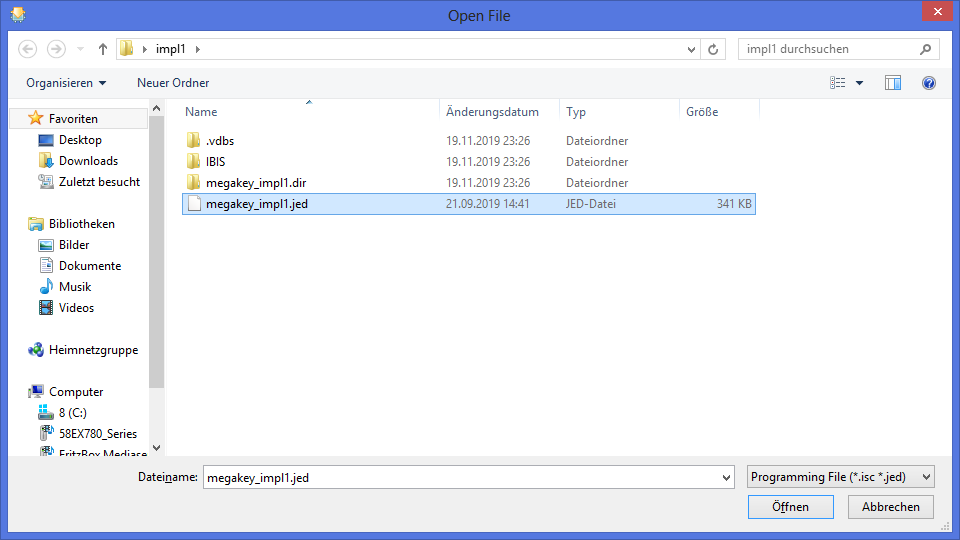
\includegraphics[width=0.8\linewidth]{images/diamond08.png}
  \end{center}
\end{minipage}


\begin{minipage}{\linewidth}
Stap 9: Selecteer kabel: \\Na een moment zou het uitvoervenster ``INFO - Operation: successful.'' moeten weergeven en zou het celletje ``Status'' groen moeten worden (dit gebeurt niet altijd).
  \begin{center}
  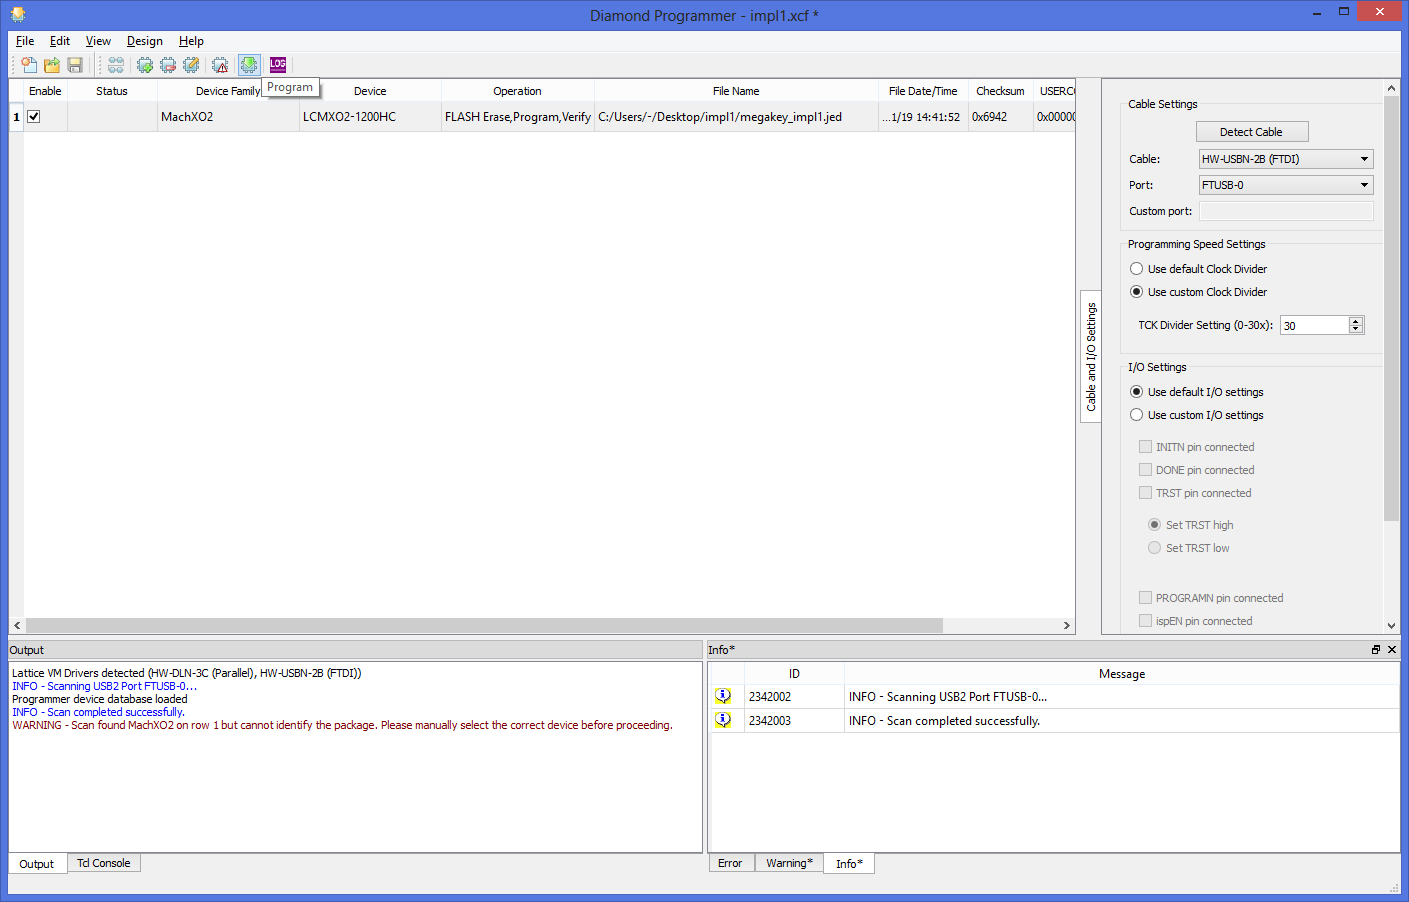
\includegraphics[width=0.8\linewidth]{images/diamond09.png}
  \end{center}
\end{minipage}

\vspace{5mm}

\begin{minipage}{\linewidth}
Stap 10: Operatie geslaagd: \\U heeft het MEGA65-toetsenbord nu succesvol geflasht. Desgewenst kunt u het project opslaan voor later gebruik.
  \begin{center}
  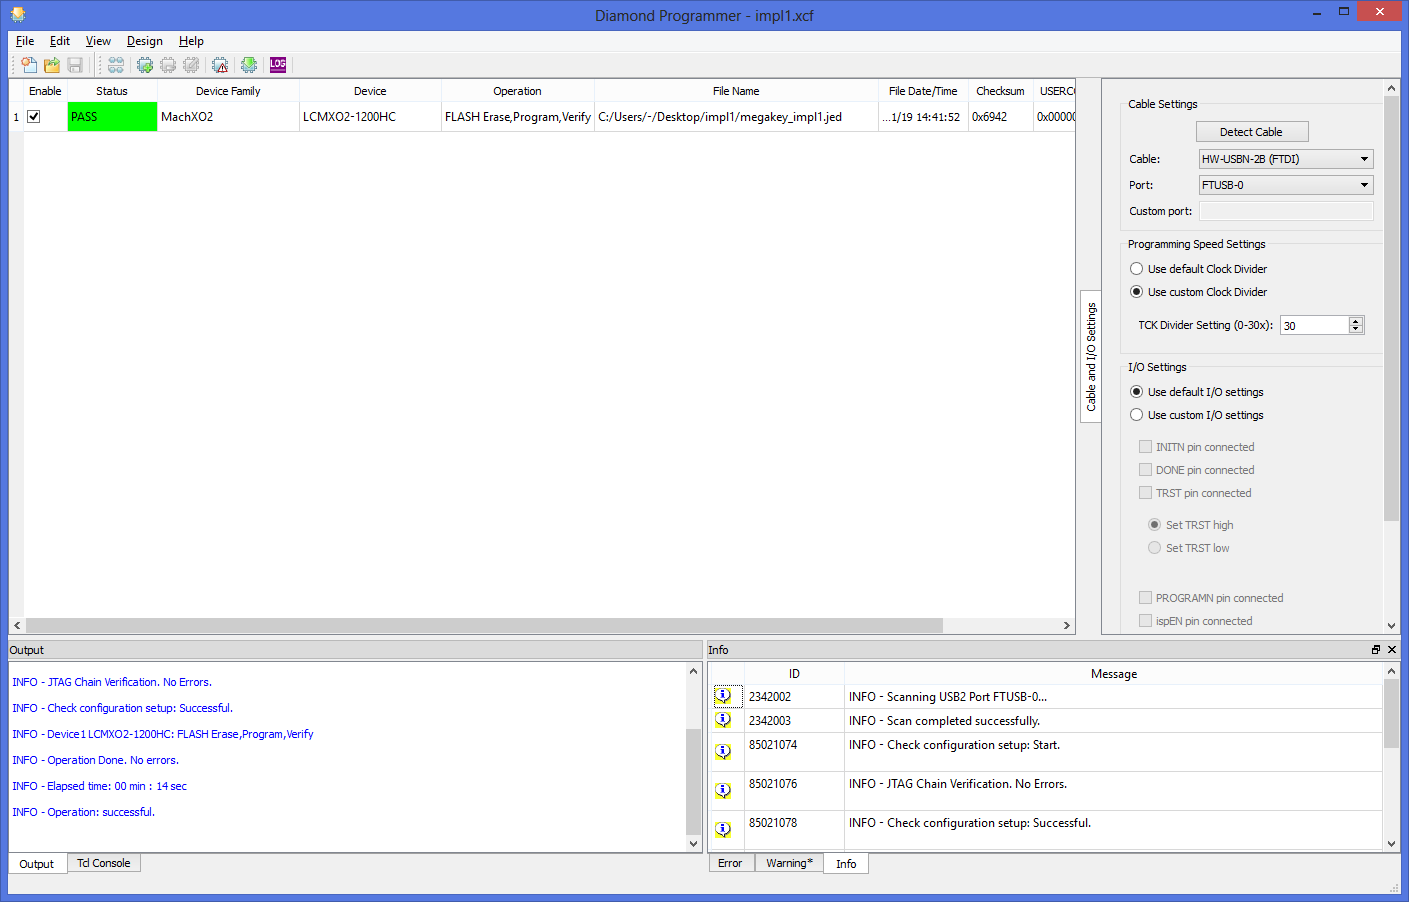
\includegraphics[width=0.8\linewidth]{images/diamond10.png}
  \end{center}
\end{minipage}


\section{Het flashen van de MAX10-FPGA op het MEGA65-moederbord met INTEL QUARTUS}
\label{sec:flashmax10}

Indien u verder wilt gaan, heeft u een TEI0004 - Arrow USB Programmer2-module nodig met het bijbehorende TEI0004-stuurprogramma geïnstalleerd en een goed functionerende installatie van Quartus Prime Programmer Lite Edition. Dit kan zowel op Windows als op Linux, maar in beide gevallen moet u de nodige USB-stuurprogramma's installeren. Sluit de MEGA65 niet aan op de netspanning en installeer de TEI0004 op de J17-connector, die zich tussen de datakabel van de diskette en de ARTIX 7-FPGA op het moederbord bevindt. De micro-USB-poort van de TEI0004 wijst in de tegenovergestelde richting van de HDMI- en LAN-aansluitingen, naar het klepje. De volgende afbeelding toont de juiste positie.

Op het PCB van een R2/R3/R3A/R4-MEGA65-moederbord moeten alle dip-schakelaars in de positie uit staan. De hoofd-FPGA van de MEGA65 mag geen geldige bitstream bevatten. De eenvoudigste manier om dit te bereiken is met een TE0790-JTAG-adapter: u kunt dan het m65-hulpprogramma vanaf een aangesloten computer gebruiken om een bitstream via JTAG te verzenden en vervolgens Control-C gebruiken om het m65-hulpprogramma te onderbreken voordat de bitstream volledig is geladen.

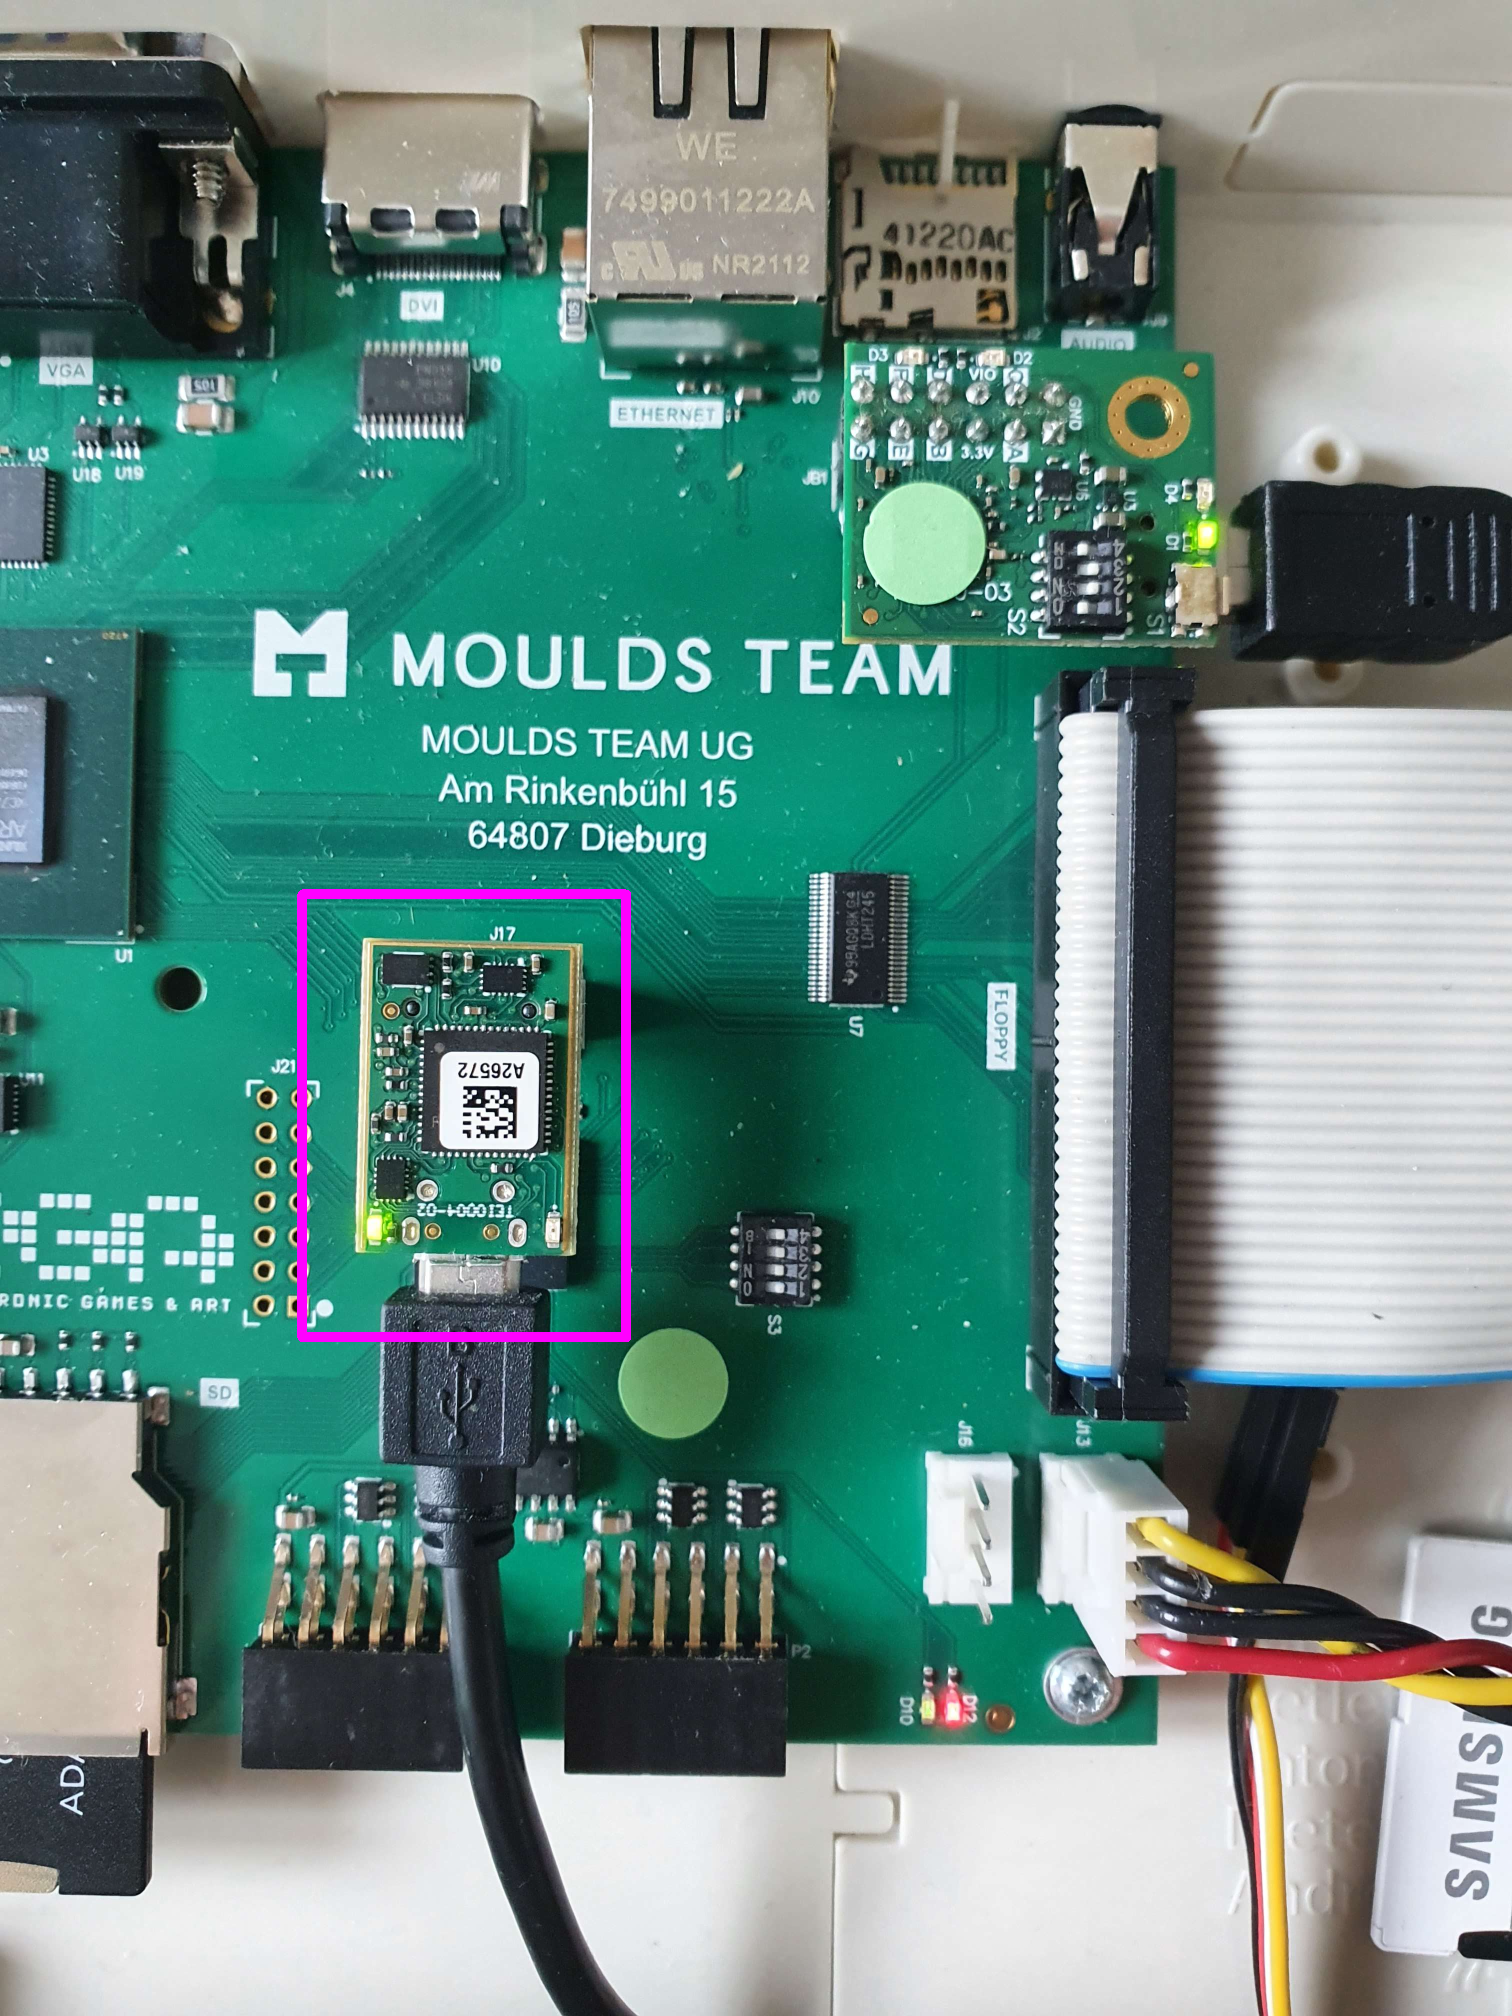
\includegraphics[width=\linewidth]{images/jtag_detail_max10.png}

Sluit uw niet-8-bit computer aan op het FPGA-programmeerapparaat met behulp van een micro-USB-kabel. Open Quartus Prime Programmer Lite Edition, dat van internet kan worden gedownload.

\begin{minipage}{\linewidth}
Stap 1: Open Quartus Prime Programmer Lite Edition: \\Klik op de knop ``Hardware Setup'' in de linkerbovenhoek van het Quartus Prime Programmer-venster.
  \begin{center}
  
\includegraphics{images/max10_01.png}
  \end{center}
\end{minipage}

\vspace{5mm}

\begin{minipage}{\linewidth}
Stap 2: Hardware-instellingen invoeren: \\In het nieuw verschenen venster kiest u onder ``Currently selected hardware'' voor ``Arrow-USB-Blaster''. Indien ``Arrow-USB-Blaster'' niet verschijnt, controleert u of de kabel en stuurprogramma's correct zijn geïnstalleerd.
  \begin{center}
  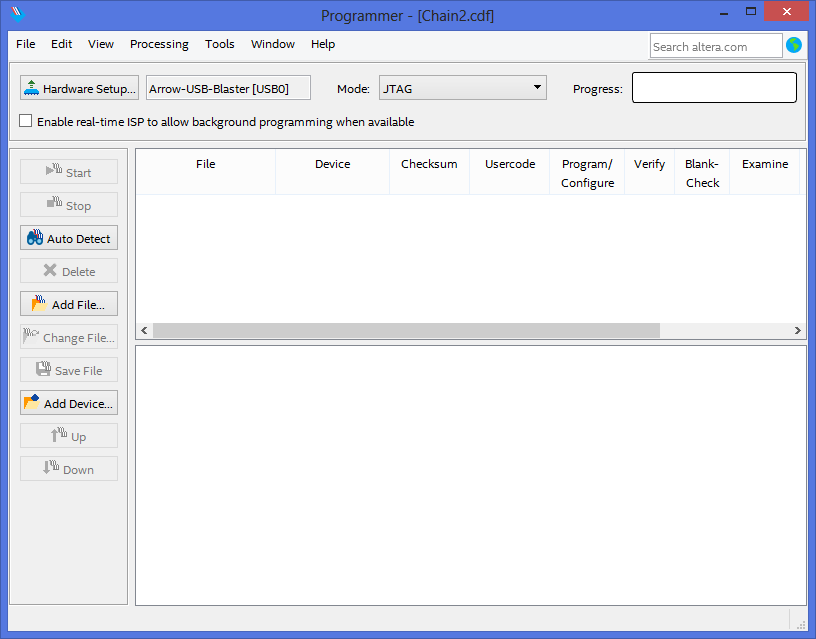
\includegraphics[width=0.8\linewidth]{images/max10_02.png}
  \end{center}
\end{minipage}


\begin{minipage}{\linewidth}
Stap 3: Selecteer Arrow USB-Blaster: \\Klik op de knop ``Add File'' in de linkerrij en kies het nieuwste bestand met de extensie ``.pof''. Klik vervolgens op ``Open''.
  \begin{center}
  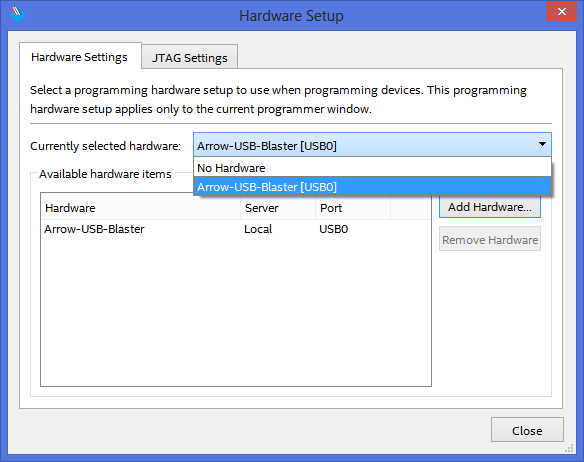
\includegraphics[width=0.8\linewidth]{images/max10_03.png}
  \end{center}
\end{minipage}


\begin{minipage}{\linewidth}
Stap 4: Selecteer programmeerbestand: \\Vink ten minste de drie vakjes onder ``Program/Configure'' aan. Het inschakelen van alle vakjes onder ``Verify'' en ``Blank-Check'' maakt het proces betrouwbaarder.
  \begin{center}
  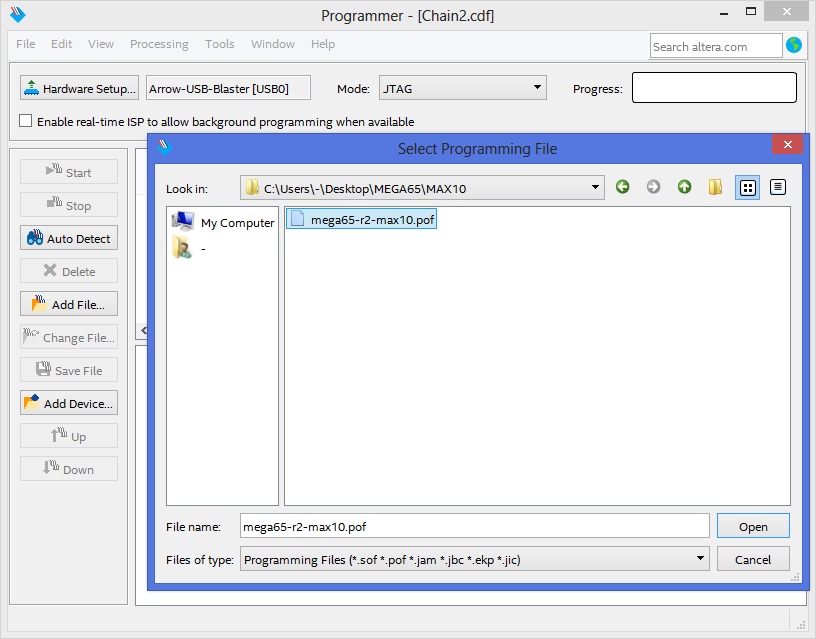
\includegraphics[width=0.7\linewidth]{images/max10_04.png}
  \end{center}
\end{minipage}

\vspace{5mm}

\begin{minipage}{\linewidth}
Stap 5: Selecteer Programmeer-/Configureeropties:
  \begin{center}
  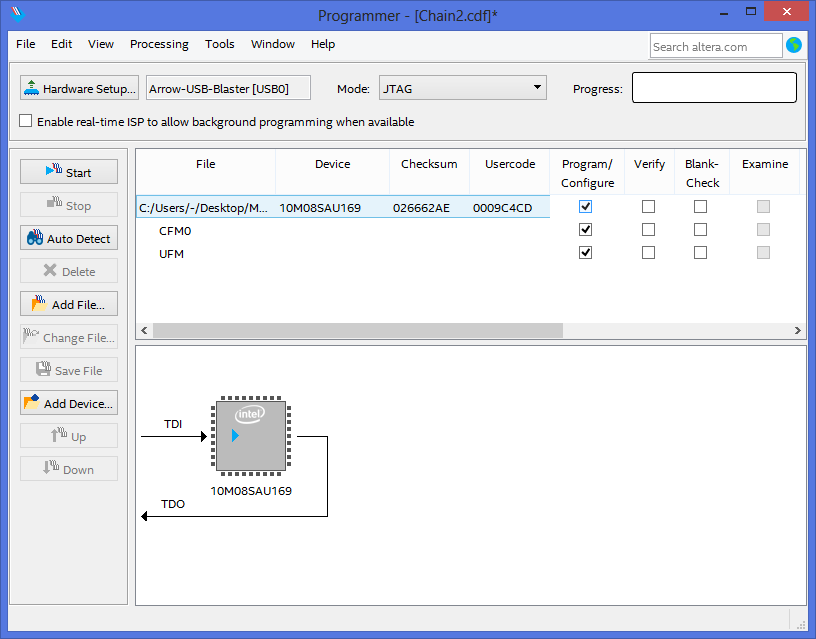
\includegraphics[width=0.7\linewidth]{images/max10_05.png}
  \end{center}
\end{minipage}

Houd de Reset-knop ingedrukt en schakel de MEGA65-computer in. Het toetsenbord gaat in de ``ambulance mode'' (blauwe flitsende lichten). Indien dit niet het geval is, is de hoofd-FPGA niet leeg: start het gehele proces opnieuw.

Klik nu op ``Start'' in de linkerrij van knoppen. De voortgangsbalk rechtsboven zou snel naar 100 procent moeten gaan en groen moeten worden. U heeft de MAX10-FPGA nu succesvol bijgewerkt.

Indien u in plaats daarvan een foutmelding ontvangt, controleer dan of de bitstream van de hoofd-FPGA is gewist en of u de reset-knop op de MEGA65 niet te vroeg heeft losgelaten. Schakel de MEGA65 uit en herhaal deze stap.

\begin{minipage}{\linewidth}
Stap 6: Programmeren geslaagd:
  \begin{center}
  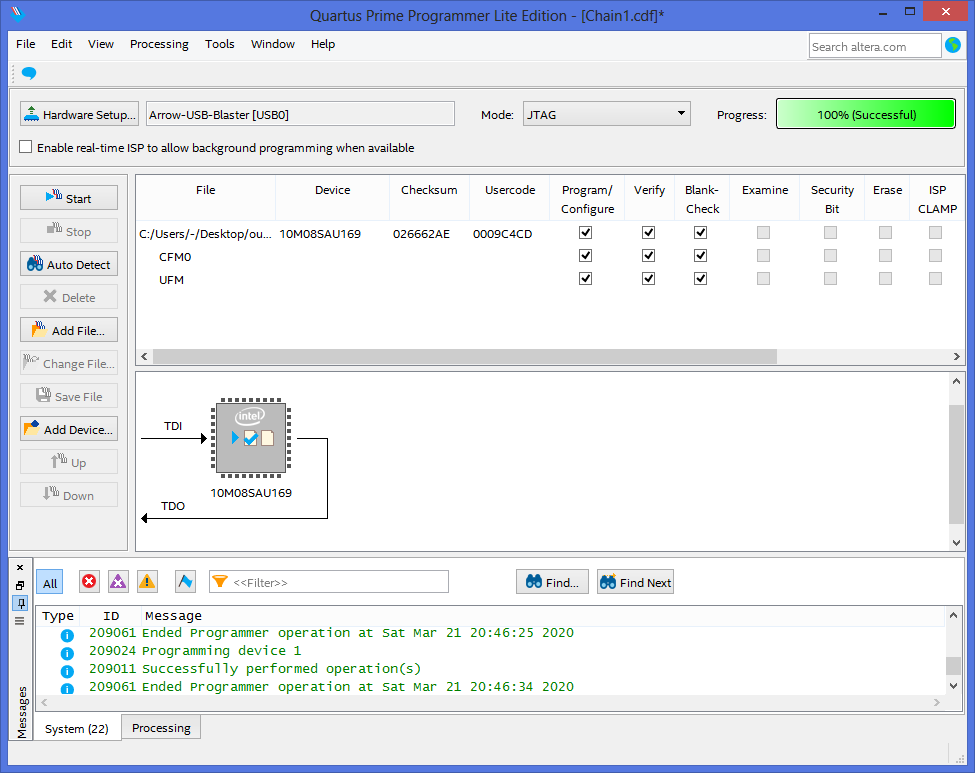
\includegraphics[width=0.8\linewidth]{images/max10_06.png}
  \end{center}
\end{minipage}

